\documentclass[11pt]{article}
\usepackage[a4paper,margin=23mm]{geometry}
\linespread{1.1}
\usepackage{amsmath,amssymb,amsthm,booktabs,longtable,array,graphicx,hyperref,microtype}
\hypersetup{colorlinks=true,linkcolor=black,citecolor=blue,urlcolor=black}\setlength{\emergencystretch}{3em}
\renewcommand{\thesection}{S\arabic{section}}\renewcommand{\theequation}{S\arabic{equation}}
\renewcommand{\thefigure}{S\arabic{figure}}\renewcommand{\thetable}{S\arabic{table}}
\newcommand{\C}{\mathbb C}\newcommand{\Z}{\mathbb Z}\newcommand{\T}{\mathbb T}
\newcommand{\R}{\mathbb R}\newcommand{\tr}{\operatorname{tr}}\newcommand{\dmin}{d_{\min}}
\newtheorem{theorem}{Theorem}\newtheorem*{theorem*}{Theorem}\newtheorem{lemma}{Lemma}\newtheorem{proposition}{Proposition}\newtheorem{corollary}{Corollary}
\renewcommand{\thetheorem}{S\arabic{theorem}}\renewcommand{\thelemma}{S\arabic{lemma}}
\renewcommand{\theproposition}{S\arabic{proposition}}\renewcommand{\thecorollary}{S\arabic{corollary}}
\title{Supplemental Material:\\Time-reversal inference with uncertain observation channels}
\author{Dev D. Goyal\\Independent researcher\\\textnormal{dvgyl@outlook.com}\\ORCID: 0009-0009-9132-744X}\date{}
\begin{document}\maketitle
\makeatletter
\renewcommand*\l@section{\@dottedtocline{1}{0em}{2.2em}}
\renewcommand*\l@subsection{\@dottedtocline{2}{1.5em}{3.8em}}
\makeatother
\tableofcontents

\subsection*{Relation to the main argument}
The main paper asks when recorded asymmetry requires an irreversible source. Sections~\ref{sec:universal}--\ref{sec:fractional} establish why unrestricted observation channels prevent that conclusion, even with exact knowledge of a finite-record law. The calibrated construction in Sec.~\ref{sec:filterextension} restricts the detector contribution. Section~\ref{cc16:section} then turns that population tolerance and the spectral cycle identity into tests by controlling finite-record errors.

The remaining proofs address whether those tests can be informative. Section~\ref{src16:proofs} propagates a reference confidence set through every allowed persistence value before bounding a detection probability. Section~\ref{cost16:section} isolates the recording cost of dependence when response and source information are already known. Section~\ref{phys16:section} derives the needed bounds from the physical models and proves the continuous-time sampling ambiguity. The study sections report how coverage, threshold size, and numerical availability affect the complete decisions. The table locates each main result within these arguments.

\begin{center}\small
\begin{tabular}{@{}p{0.30\textwidth}p{0.60\textwidth}@{}}\toprule
Main-text result & Supporting material \\\midrule
Theorem 1: finite-law ambiguity & Section~\ref{sec:universal}, Theorem~\ref{thm:mc-main} and Proposition~\ref{prop:mc-uniform}; real-delay extension in Sec.~\ref{sec:fractional}, Theorem~\ref{thm:fractional}. \\
Calibrated population tolerance & Section~\ref{sec:filterextension}, including response confidence and supplied covariance information. \\
Theorems 2--3: finite-record tests & Section~\ref{cc16:section}: Theorem~\ref{cc16:geometric} gives the calibrated rule; Theorem~\ref{cc16:cycle-theorem} gives the cycle rule. \\
Theorem 5 and the detection example & Section~\ref{src16:proofs}, Complete definitions and statements precede Sec.~S5.1. Proofs of the hull bound and detection example are in Secs.~S5.4 and S5.9--S5.10. \\
Theorem 4: recording cost & Section~\ref{cost16:section}, Theorems~\ref{cost16:necessary} and~\ref{cost16:sufficient}. \\
Physical examples & Section~\ref{phys16:section}. \\
Synthetic performance & Sections~\ref{study16:section}--\ref{study16:tables} give design, results, diagnostics, and fixed comparison tables. Section~\ref{study16:onesided} summarizes earlier comparisons that use different designs. \\\bottomrule
\end{tabular}
\end{center}

\subsection*{Notation}
A covariance envelope bounds the covariance of the complete record in every linear direction. A confidence hull is the smallest closed interval that contains a confidence set. A filter bank is a finite list of common filters declared before observation.

\begin{center}\small
\begin{tabular}{@{}p{0.22\textwidth}p{0.68\textwidth}@{}}\toprule
Symbol & Meaning \\\midrule
$C_{ij}(k)$ & Observed covariance $\operatorname{Cov}\{Y_i(t+k),Y_j(t)\}$. Source covariances are identified explicitly. \\
$F,S,\mu$ & Observed spectral matrix, source spectral matrix, and source spectral measure. \\
$f_n$ & Frobenius norm of the two-time reflection coefficient matrix. It differs from the spectral matrix $F$. \\
$K_B$ & Cumulative-sum matrix for centered candidate innovations. \\
$\omega,\mathcal S$ & Frequency and source spectral ceiling-to-floor ratio. \\
$q,K_i$ & Standardized full covariance envelope and channel-scaled diagonal envelope entries. \\
$B_{ij},L$ & Cycle bias allowance and lag cutoff. \\
$r,\widehat r$ & True phase tolerance and calibrated upper bound. \\
$V_i,D_i,D_{\rm g}$ & Centered recorded variance, its upper confidence bound, and the geometric mean of the two bounds. \\
$\phi,\psi,a_j$ & True source persistence, candidate persistence, and fixed filter coefficient. \\
$[\ell,u],\Lambda(x)$ & Source confidence hull and $\Lambda(x)=(1+x)/(1-x)$. \\
$d_{\mathrm{mom}}$ & Dimension of the finite retained-covariance space. \\
$D(\psi),Q(\psi),R_n(\psi)$ & Centered innovation energy, cumulative innovation energy, and their pivot ratio. \\
$N,n,M$ & Record length, number of innovations or adjacent pairs, and bank size. Each construction gives their exact relation. The delay construction uses $M$ as its integer separation parameter. \\
$\eta_i,\eta_H$ & Per-sample recording and calibration error bounds. \\
$\xi,a,w$ & Physical channel correlation, rotational drift decay, and rotational frequency coefficient. The main text writes the last two as $\lambda,\nu$. \\
$\log,\log_2$ & Natural logarithm and base-two logarithm. \\\bottomrule
\end{tabular}
\end{center}

The reflection sign convention is $U_t=Y_1(t)+Y_1(t+1)$ and $W_t=Y_2(t)-Y_2(t+1)$. Its uncentered mean is $C_{12}(1)-C_{12}(-1)$. All tests use its absolute value. Spectral densities on the discrete-time torus use $d\omega/(2\pi)$. Continuous-time densities use Lebesgue measure as stated in their construction.

% Requires amsmath, amssymb, and amsthm.
\section{Channel-specific delays for finite Gaussian records}\label{sec:universal}
\newcommand{\MC}{\mathcal C}
\newcommand{\MD}{\mathcal D}
\newcommand{\MT}{\mathbb T}
\newcommand{\MR}{\mathbb R}
\newcommand{\MS}{\mathbb S}

A finite Gaussian law is determined by its retained means and covariances. The construction below matches those quantities exactly with a reversible source and channel-specific delays. The source and its unobserved extension can depend on the target law.

The difficulty is to satisfy reversibility and exact covariance matching at the same time. A real source spectrum has no complex channel phases of its own. Separated delays can approximate the phases of each rank-one spectral mass, but an approximation does not give the same finite law. We therefore apply the approximation to nearby valid covariance arrays that surround the target. Small changes preserve this containment, so a positive mixture of their outputs matches the target exactly. This also permits smoothing the masses into a strictly positive density before taking the final mixture. The notation below specifies the finite set of moments that must be preserved.

Let $m,N\ge1$ be integers. A retained covariance array consists of real
numbers $C_{ij}(k)$, $1\le i,j\le m$, $|k|\le N-1$, with
$C_{ji}(-k)=C_{ij}(k)$. Its block Toeplitz matrix is
$\Gamma_N(C)=(C_{ij}(t-u))_{(t,i),(u,j)}$, $0\le t,u<N$.
The cone $\MC_{m,N}$ contains the arrays for which $\Gamma_N(C)\succeq0$.
Use the independent coordinates $C_{ii}(k)$, $0\le k<N$, and
$C_{ij}(k)$, $i<j$, $|k|<N$. Their real dimension is
\begin{equation}\label{eq:mc-dimension}
 d_{\mathrm{mom}}=mN+\binom m2(2N-1)=m^2N-\frac{m(m-1)}2.
\end{equation}
Throughout, $\|C\|_{\mathrm{coord}}$ is the maximum absolute value of
these independent coordinates. Each entry of $\Gamma_N(C)$ is one
coordinate, possibly repeated. In particular
\begin{equation}\label{eq:mc-entry-norm}
 \|\Gamma_N(C)\|_{\mathrm{op}}\le mN\|C\|_{\mathrm{coord}}.
\end{equation}
Spectral densities are with respect to $\nu(d\omega)=d\omega/(2\pi)$
on $\MT=\MR/(2\pi\mathbb Z)$, with moment convention
$C_{ij}(k)=\int e^{ik\omega}\mu_{ij}(d\omega)$.
For integer channel delays $d=(d_1,\ldots,d_m)$ put
\[
 D_d(\omega)=\operatorname{diag}(e^{-id_1\omega},\ldots,e^{-id_m\omega}).
\]
Thus $Y_i(t)=X_i(t-d_i)$ has spectral measure $D_d\mu D_d^*$ and
\begin{equation}\label{eq:mc-delay-sign}
 C^Y_{ij}(k)=C^X_{ij}(k-d_i+d_j).
\end{equation}

\begin{theorem}[Common hierarchical delays]\label{thm:mc-main}
Let $C^{(1)},\ldots,C^{(s)}\in\MC_{m,N}$ be a nonempty finite collection
with $\Gamma_N(C^{(c)})\succ0$. Write
$\lambda_c=\lambda_{\min}(\Gamma_N(C^{(c)}))$ and
$v_c=\max_i C^{(c)}_{ii}(0)$.
If $m\ge2$, every integer $M\ge2$ satisfying
\begin{equation}\label{eq:mc-threshold}
 M-1>\pi(N+1)(2d_{\mathrm{mom}}-1)
       \max_{1\le c\le s}\left(\frac{2mN v_c}{\lambda_c}+1\right)
\end{equation}
admits the following simultaneous realizations with the shared delay vector
\begin{equation}\label{eq:mc-delays}
 (d_1,\ldots,d_m)=(M,M^2,\ldots,M^{m-1},0).
\end{equation}
For each $c$ there is a real stationary reversible Gaussian process
$X^{(c)}$, whose spectral density $S_c$ is a real, even, symmetric matrix
trigonometric polynomial, such that $S_c(\omega)\succeq\epsilon I_m$ for
all $\omega$ and a common $\epsilon>0$. The delayed process
$Y^{(c)}_i(t)=X^{(c)}_i(t-d_i)$ has retained covariance exactly $C^{(c)}$.
The density degrees have a common finite upper bound $L$, and each
source is $L$-dependent. For every coordinate,
\begin{equation}\label{eq:mc-variance}
 \operatorname{Var}(X^{(c)}_i(t))=C^{(c)}_{ii}(0).
\end{equation}
Consequently these are exact realizations of the retained Gaussian laws,
with zero added errors. Arbitrary constant mean vectors are preserved by
assigning the same mean vectors to the sources. Each delay response has
unit coefficient norm.

For $m=1$ the same conclusion holds with $d_1=0$, without a restriction
on $M$. For $N=1$ it holds for every prescribed vector of nonnegative
integer delays, without condition~\eqref{eq:mc-threshold}.
\end{theorem}

\begin{proof}
We first reduce the retained law to finitely many rank-one spectral masses. We then move their frequencies so the prescribed delays approximate their phases. Finally, convex mixtures correct the retained moments without a signed spectral perturbation that could destroy positivity.

\emph{Finite spectral representation.}
Every $C\in\MC_{m,N}$ has a finite positive semidefinite matrix spectral
measure obeying $\mu(-A)=\overline{\mu(A)}$ and the prescribed retained
moments. To see this, take a real Gram representation
$C_{ij}(t-u)=\langle v_{t,i},v_{u,j}\rangle$ in a real space $E$ of
dimension $\operatorname{rank}\Gamma_N(C)$. The map
$v_{t,i}\mapsto v_{t+1,i}$ on the span with $0\le t<N-1$ is well defined
and isometric: Toeplitz equality preserves the squared norm of every
linear combination, including a zero combination. The domain and range have equal dimension. Thus extend this map to a
real orthogonal map $U:E\to E$. When $N=1$, one may simply take $U=I_E$. Then
$v_{t,i}=U^t v_{0,i}$ for the retained times. The spectral decomposition
of the complexification of $U$ supplies the measure. More explicitly,
with a complex inner product linear in its first argument, let
$P_\omega$ be the eigenspace projection for $e^{i\omega}$ and set
$W_{\omega,ij}=\langle P_\omega v_{0,i},P_\omega v_{0,j}\rangle$.
These are Hermitian positive semidefinite matrices and
$C_{ij}(k)=\sum_\omega e^{ik\omega}W_{\omega,ij}$.
Realness of $U$ pairs conjugate eigenspaces. The endpoint matrices at
$0$ and $\pi$ are real. There are at most $\dim E\le mN$ distinct nodes.

Equivalently, write the real moments as a finite sum
\begin{equation}\label{eq:mc-paired-atoms}
 C_{ij}(k)=\sum_\ell\operatorname{Re}
                (e^{ik\omega_\ell}v_{\ell,i}\overline{v_{\ell,j}}).
\end{equation}
Here a conjugate pair of matrix masses has first been combined into its
half-circle mass and then split into rank-one matrices; endpoint masses
can be split into real rank-one matrices. Each term in
\eqref{eq:mc-paired-atoms} represents the full-circle measure
$(vv^*\delta_\omega+\overline v v^{\mathsf T}\delta_{-\omega})/2$.
In particular,
\begin{equation}\label{eq:mc-rankone-budget}
 \sum_\ell |v_{\ell,i}|^2=C_{ii}(0),\qquad
 \sum_\ell |v_{\ell,i}||v_{\ell,j}|
 \le\sqrt{C_{ii}(0)C_{jj}(0)}.
\end{equation}

\emph{Simultaneous phase approximation.}
The retained moments change little under a small frequency displacement. The hierarchical delays make such a displacement sufficient to set one channel phase at a time, with decreasing effects on phases already set.
Fix $m\ge2$, $M\ge2$, an arbitrary real representative $\omega$ of a
frequency, and phases $p_1,\ldots,p_{m-1}$ on the unit circle. Starting
with $\theta_0=\omega$, choose $\theta_j$ nearest to $\theta_{j-1}$ among
the real solutions of $e^{-iM^j\theta_j}=p_j$. Their spacing is
$2\pi/M^j$, so $|\theta_j-\theta_{j-1}|\le\pi/M^j$. Put
$\theta=\theta_{m-1}$. Then
\begin{align}
 |\theta-\omega|&\le\sum_{j=1}^{m-1}\frac\pi{M^j}
                         \le\frac\pi{M-1},\label{eq:mc-grid-freq}\\
 |e^{-iM^i\theta}-p_i|
 &\le M^i|\theta-\theta_i|
 \le\pi\sum_{r=1}^{m-1-i}M^{-r}
 \le\frac\pi{M-1},\quad 1\le i<m.\label{eq:mc-grid-phase}
\end{align}
The sum in the last line is empty for $i=m-1$, whose phase is exact.
Frequencies are reduced modulo $2\pi$ only after this construction;
no restriction to a half-circle is imposed on $\theta$.

Apply this construction separately to each vector $v$ in
\eqref{eq:mc-paired-atoms}. Multiplying $v$ by a global unit complex
number does not change $vv^*$. If $v_m\ne0$, use this freedom to make
$v_m$ real nonnegative. If $v_m=0$, use any global phase. Set
$a_i=|v_i|$ and write $v_i=p_i a_i$, taking $p_m=1$ and assigning any
unit phase to a zero coordinate. Thus $v=\operatorname{diag}(p)a$ with
$a\in[0,\infty)^m$ even when some coordinates vanish. Give the source
the real-even measure
\[
 \frac12 aa^{\mathsf T}\delta_\theta+
 \frac12 aa^{\mathsf T}\delta_{-\theta}.
\]
Its delayed moment contribution is
$\operatorname{Re}(e^{ik\theta}q_i\overline q_j)a_i a_j$, where
$q_i=e^{-id_i\theta}$ and $q_m=1$. At a coincident reflected pair
($\theta=0$ or $\pi$ modulo $2\pi$), the two half masses add to one
mass, and every $q_i$ is real because $d_i$ is integral. The output mass
there is therefore real and admissible. At every other frequency the
reflected output mass is the conjugate of the first one. These
observations also cover a frequency displaced across an endpoint.

For $|k|\le N-1$, equations~\eqref{eq:mc-grid-freq}--\eqref{eq:mc-grid-phase}
give
\begin{align*}
 |e^{ik\theta}q_i\overline q_j-e^{ik\omega}p_i\overline p_j|
 &\le |k||\theta-\omega|+|q_i-p_i|+|q_j-p_j|\\
 &\le\frac{\pi(N+1)}{M-1}.
\end{align*}
Combining all the real source atoms gives an output $\widetilde C$ with
\begin{equation}\label{eq:mc-approx}
 \|\widetilde C-C\|_{\mathrm{coord}}
 \le\frac{\pi(N+1)V}{M-1},\qquad
 \widetilde C_{ii}(0)=C_{ii}(0),\quad
 V=\max_i C_{ii}(0),
\end{equation}
by~\eqref{eq:mc-rankone-budget}. The same delay vector works for every
such array. Splitting into rank-one terms before moving frequencies is
essential; no simultaneous diagonal dephasing of a general matrix mass
has been assumed.

\emph{A simplex with an explicit perturbation margin.}
The approximate output need not equal the target. To correct this error while retaining positive source measures, we approximate several arrays around the target. A simplex is their convex hull. The margin below ensures that the target stays inside that hull after the approximation.
For a target $C^{(c)}$, use the natural coordinate basis $E_1,\ldots,E_{d_{\mathrm{mom}}}$
and write
\[
 a_c=\frac{\lambda_c}{2mN},\quad
 B_c=v_c+a_c,\quad
 V_{c,0}=C^{(c)}-a_c\sum_{j=1}^{d_{\mathrm{mom}}} E_j,\quad
 V_{c,j}=C^{(c)}+a_cE_j\quad(1\le j\le d_{\mathrm{mom}}).
\]
Every matrix perturbation has operator norm at most $mNa_c=\lambda_c/2$
by~\eqref{eq:mc-entry-norm}; hence all vertices are positive definite.
Their maximal coordinate variances are at most $B_c$.
This simplex contains the coordinate cube with center $C^{(c)}$ and
radius
\begin{equation}\label{eq:mc-radius}
 \rho_c=\frac{a_c}{2d_{\mathrm{mom}}-1}.
\end{equation}
Indeed the barycentric coordinates of displacement $x$ are
\[
 \alpha_0=\frac{1-\sum_j x_j/a_c}{d_{\mathrm{mom}}+1},\qquad
 \alpha_j=\alpha_0+x_j/a_c.
\]
For $\|x\|_\infty\le\rho_c$, the numerator of $\alpha_0$ is at least
$1-d_{\mathrm{mom}}/(2d_{\mathrm{mom}}-1)\ge0$, and the numerator of $\alpha_j$ is at least
$1-(2d_{\mathrm{mom}}-1)/(2d_{\mathrm{mom}}-1)=0$. These inequalities also hold for $d_{\mathrm{mom}}=1$.

If each vertex of this simplex moves by at most $\eta<\rho_c$ in
coordinate norm, its new convex hull contains the cube of radius
$\rho_c-\eta$ about $C^{(c)}$. For each linear functional $u$, the hull's support function drops by at most
$\eta\|u\|_1$. The original cube provides support
$u\cdot C^{(c)}+\rho_c\|u\|_1$. The
support-function characterization of containment proves the claim.
In particular the perturbed hull is full dimensional. Since it has
$d_{\mathrm{mom}}+1$ vertices, they are affinely independent and $C^{(c)}$ has strictly
positive barycentric coordinates.

Apply~\eqref{eq:mc-approx} to the vertices. The coordinate errors are at
most $\eta_c=\pi(N+1)B_c/(M-1)$. Condition~\eqref{eq:mc-threshold} is
exactly $\eta_c<\rho_c$ for each $c$. Thus every target belongs to the
strict interior of a simplex of outputs of finite reversible source
measures under the prescribed delay vector. The strict inequality leaves a positive margin for the next step. Without that margin, smoothing could move the output vertices so that their convex hull no longer contains the target.

\emph{Positive polynomial source densities at fixed delays.}
The convex hull currently contains outputs of atomic source measures. Smoothing gives polynomial densities and adding white power makes them strictly positive. Both operations change the moments, so they must fit inside the remaining containment margin before the exact mixture is chosen.
Now hold $M$ and the delay vector fixed. Denote the source measure at a
perturbed vertex by $\mu_{c,j}$. For $L\ge0$ let
\[
 F_L(\omega)=\frac1{L+1}\left|\sum_{r=0}^L e^{ir\omega}\right|^2
   =\sum_{|r|\le L}\left(1-\frac{|r|}{L+1}\right)e^{ir\omega}.
\]
This is a real, even, nonnegative trigonometric polynomial of integral
one against $\nu$. For $\epsilon>0$ define
\begin{equation}\label{eq:mc-smooth}
 S_{c,j}^{L,\epsilon}(\omega)
   =\int F_L(\omega-\theta)\mu_{c,j}(d\theta)+\epsilon I_m.
\end{equation}
These are real-even symmetric polynomial densities bounded below by
$\epsilon I_m$. For each fixed integer $r$, convolution multiplies the
$r$th source moment by $1-|r|/(L+1)$ when $L\ge|r|$. Added white power
changes only the zero-lag diagonal moments. By~\eqref{eq:mc-delay-sign},
only source lags of absolute value at most
\begin{equation}\label{eq:mc-Q}
 Q=N-1+M^{m-1}
\end{equation}
enter the retained output moments. Thus the smoothed output vertices
converge to their unsmoothed counterparts as $L\to\infty$ and
$\epsilon\to0$. There are finitely many vertices, so finite common
$L$ and positive common $\epsilon$ preserve all strict simplex
containments. With their resulting positive barycentric coefficients
$\beta_{c,j}$, put $S_c=\sum_{j=0}^{d_{\mathrm{mom}}}\beta_{c,j}S_{c,j}^{L,\epsilon}$.
The coefficients sum to one, so $S_c\succeq\epsilon I_m$, and linearity
of the output moment map gives exactly $C^{(c)}$.

These matrix densities define stationary real Gaussian processes.
Their source covariance matrices are real symmetric and even in the
lag, which makes their Gaussian finite-dimensional distributions
invariant under time reversal. Polynomial degree at most $L$ makes
all source covariances at $|k|>L$ vanish. Joint Gaussianity then gives
independence for any finite sets of source variables separated in time
by more than $L$; a monotone-class argument gives independence of the
corresponding generated sigma fields. Thus the sources are $L$-dependent.
At every frequency, $D_d$ is diagonal unitary and hence leaves the
diagonal spectral measures unchanged. Exact matching of the retained
zero-lag diagonal moments therefore proves~\eqref{eq:mc-variance}.

\emph{Scalar records and records of length one.}
For $m=1$, the finite spectral representation has an even scalar
measure and already gives a reversible source at every
simplex vertex without a phase approximation or delay. The same
smoothing and simplex correction complete the argument.
For $N=1$ and any fixed prescribed integer delay vector, represent each
positive definite simplex vertex by its matrix mass at frequency zero.
All delay factors are one there, so the vertex is already represented
exactly by a real-even source measure. Holding the delays fixed,
smoothing and simplex correction again give the claimed conclusion.
For zero delays alone, white sources suffice directly.
\end{proof}

\begin{proposition}[Uniform bounds at a fixed chosen delay]\label{prop:mc-uniform}
Fix $m\ge2$, $N\ge1$, $\lambda_*>0$ and $v_*<\infty$. The preceding
conclusion applies to every target satisfying
$\Gamma_N(C)\succeq\lambda_*I_{mN}$ and $\max_iC_{ii}(0)\le v_*$,
using a common delay parameter $M$ whenever
\[
 M\ge2,\qquad M-1>\pi(N+1)(2d_{\mathrm{mom}}-1)
                          \left(\frac{2mN v_*}{\lambda_*}+1\right).
\]
The targets may be an infinite family; their sources may differ. In
particular this applies uniformly to every compact subset of the
positive definite moment cone. For each fixed such $M$, the sources
can also have common finite polynomial degree and a common positive
spectral lower bound. One sufficient explicit choice is as follows:
\begin{gather*}
 a=\frac{\lambda_*}{2mN},\quad B=v_*+a,\quad
 \rho=\frac a{2d_{\mathrm{mom}}-1},\quad
 \eta=\frac{\pi(N+1)B}{M-1},\quad b=\rho-\eta>0,\\
 Q=N-1+M^{m-1},\qquad \epsilon=\frac b3,\qquad
 L\ge Q,\qquad L+1>\frac{3QB}{b}.
\end{gather*}
Every source obtained by the construction then obeys
$S_C(\omega)\succeq\epsilon I_m$ and has degree at most $L$.
These are sufficient bounds, not minimum resource requirements; they
depend on the fixed chosen $M$.
\end{proposition}
\begin{proof}
Use the same $a,B,\rho$ for the simplex about every target. The atomic
approximation preserves each source diagonal mass, so the source
measure at every vertex has coordinate variances at most $B$. For any
integer $r$, its matrix moment satisfies
\[
 |\widehat\mu_{ij}(r)|\le
   \sqrt{\widehat\mu_{ii}(0)\widehat\mu_{jj}(0)}\le B.
\]
For the finite real source measures constructed above, this follows
directly by summing the absolute values of their rank-one contributions
and applying Cauchy--Schwarz. At a required source lag $|r|\le Q$,
Fej\'er smoothing therefore changes a moment by at most $QB/(L+1)$.
The added white density changes each output coordinate by at most
$\epsilon$; for diagonal delays it affects only a zero-lag diagonal
coordinate. The total smoothed vertex displacement from the original
simplex is consequently at most
\[
 \eta+\frac{QB}{L+1}+\epsilon
 <\eta+\frac b3+\frac b3<\rho.
\]
The simplex argument applies separately to every target with the same
$M,L,\epsilon$. Compactness is not otherwise needed: a compact subset
of the positive definite cone supplies the displayed uniform eigenvalue
and variance bounds by continuity.
\end{proof}

\paragraph{Scope.}
The theorem concerns exact finite Gaussian record laws. It permits the
source law to vary with the target and with the selected delays. It does
not assert equality to a prescribed full-process law, a smallest delay,
a source range independent of $M$, or equality of non-Gaussian laws
from covariance matching. Its maximal constructed delay $M^{m-1}$ is
a sufficient choice. Polynomial source spectra make every covariance vanish beyond a finite lag.

\subsection{Limits of the finite-record construction}
The rank-one decomposition cannot in general be replaced by dephasing
a whole matrix mass. For example, with $r=2/5$ the Hermitian matrix
\[
 W=\begin{pmatrix}1&r&-ir\\r&1&r\\ir&r&1\end{pmatrix}
\]
has least eigenvalue at least $1-2r=1/5$. Its cycle product
$W_{12}W_{23}W_{31}=ir^3$ is invariant under diagonal unitary
congruence. A real symmetric matrix has a real cycle product, so no
such congruence makes $W$ real. Moving its rank-one pieces separately
avoids this obstruction.

Strict positive definiteness of the retained target is necessary for
the asserted positive source floor. If $S_X\succeq\epsilon I_m$, then
$D_dS_XD_d^*\succeq\epsilon I_m$. For any block vector $u$, integration
of its Fourier polynomial and Parseval's identity give
$u^{\mathsf T}\Gamma_N(C^Y)u\ge\epsilon\|u\|_2^2$.
A singular retained covariance therefore cannot have this type of
realization. This does not exclude realizations with singular spectra.

A prescribed full-process spectrum imposes further restrictions.
Consider a bivariate spectrum with unit diagonal and cross entry
\[
 f(\omega)=\frac14\left(1+\frac i2\sin\omega\right).
\]
It has the real-process conjugation symmetry and is uniformly positive,
since $|f(\omega)|\le\sqrt5/8<1$. A reversible-source explanation by
integer delays would require $e^{i\Delta\omega}f(\omega)$ to be real,
where $\Delta=d_1-d_2\in\mathbb Z$. The derivative of its imaginary
part at zero is $(\Delta+1/2)/4$, which never vanishes for integer
$\Delta$. Hence this full-process law has no such explanation, although
every finite retained covariance is positive definite and satisfies
Theorem~\ref{thm:mc-main}. The source and the unobserved output extension
may depend on the chosen finite record.

The source-degree bound in Proposition~\ref{prop:mc-uniform} also must
depend on the selected delay. For $m\ge2$, fix a temporally white
positive definite target whose contemporaneous covariance is the identity except for
$C_{1m}(0)=C_{m1}(0)=r$, with $0<|r|<1$. Under the hierarchical delays,
exactness requires $C^X_{1m}(-M)=r$. A polynomial source spectrum of
degree $L$ has zero moments at all lags of magnitude greater than $L$,
so necessarily $L\ge M$. Thus no bound independent of $M$ is possible,
even for a singleton compact family of targets. The bounds uniform over
targets in Proposition~\ref{prop:mc-uniform} hold at each fixed $M$.

\subsection{A linear-delay construction under an observable covariance margin}\label{sec:linear-delay}
A stronger condition on the retained covariances permits an explicit construction with linearly spaced delays. The comparison matrix below combines lower bounds for the auto spectra with absolute bounds for the cross spectra. Its positive definiteness is sufficient to keep the constructed source spectrum positive. This gives a direct construction for a smaller covariance class than the universal theorem.

For each condition $c$, put $H=N-1$, $v_{ci}=C^{(c)}_{ii}(0)$ and define
\[
a_{ci}=v_{ci}-2\sum_{k=1}^{H}|C^{(c)}_{ii}(k)|,\qquad
(B_c)_{ij}=2\sum_{k=-H}^{H}|C^{(c)}_{ij}(k)|\quad(i\ne j),
\]
with $(B_c)_{ii}=0$. Let
\[
Q_c=\operatorname{diag}(a_{c1},\ldots,a_{cm})-B_c.
\]
Assume $N,m\ge2$ and $Q_c\succ0$ in every condition. This sufficient condition uses only retained covariances. Positive definiteness of the observed record alone does not imply this condition. The simpler inequalities $a_{ci}>\sum_{j\ne i}(B_c)_{ij}$ imply $Q_c\succ0$ by strict diagonal dominance.

\begin{theorem}[Direct positive spectra with linearly spaced delays]\label{thm:linear-delay}
For any nonempty finite family satisfying the displayed condition, the common
channel delays
\[
 d_i=(m-i)(N-1),\qquad 1\le i\le m,
\]
realize all retained laws exactly with zero errors and reversible
Gaussian sources whose real symmetric even trigonometric polynomial spectral
densities have degree at most $m(N-1)$ and are bounded below by
$\gamma I_m$, where $\gamma=\min_c\lambda_{\min}(Q_c)>0$.
Source coordinate variances equal the observed variances. In particular
the maximum delay is $(m-1)(N-1)$, linear in the retained horizon at
fixed channel count.
\end{theorem}
\begin{proof}
It suffices to construct one condition; omit its superscript. Put
$H=N-1$ and $\Delta_{ij}=d_i-d_j=(j-i)H$ for $i<j$.
Define
\[
 S_{ii}(\omega)=v_i+2\sum_{k=1}^{H}C_{ii}(k)\cos(k\omega).
\]
For $i<j$, the numbers $n_k=\Delta_{ij}-k$, $-H\le k\le H$,
are distinct nonnegative integers. Define
\[
 S_{ij}(\omega)=S_{ji}(\omega)
 =\sum_{k=-H}^{H}(2-\mathbf1_{n_k=0})C_{ij}(k)\cos(n_k\omega).
\]
Fourier orthogonality against $d\omega/(2\pi)$ gives source moment
$R_{ij}(k-\Delta_{ij})=C_{ij}(k)$ for each retained $k$.
The coefficient one at frequency zero is required because its integral
is one, whereas $\cos^2(n\omega)$ integrates to $1/2$ for $n>0$.
The diagonal source moments also match the observed auto moments, which
pure delays preserve. Symmetry and stationarity give the corresponding
$j,i$ output entries.

Pointwise, $S_{ii}(\omega)\ge a_i$ and $|S_{ij}(\omega)|\le B_{ij}$. For every real vector $u$, write $|u|$ for its componentwise absolute value. Then
\[
u^{\mathsf T}S(\omega)u
\ge\sum_i a_i u_i^2-\sum_{i\ne j}B_{ij}|u_i||u_j|
=|u|^{\mathsf T}Q|u|
\ge\lambda_{\min}(Q)\|u\|_2^2.
\]
This positive real-even density defines a stationary reversible Gaussian
source. Its degree is at most
$\max_{i<j}(\Delta_{ij}+H)=mH$. Thus its covariances vanish beyond
$mH$, and its Gaussian process is $mH$-dependent. All zero-lag diagonal
moments equal $v_i$. Apply this construction independently to each
condition, preserving the same delays and taking the minimum floor.
\end{proof}
The comparison-matrix condition is unchanged by nonzero rescaling of individual channels. If $D$ is the diagonal scaling matrix, the transformed comparison matrix is $|D|Q_c|D|$, so positive definiteness is equivalent. This condition can hold when a row-dominance inequality fails. For example, white auto-covariances with variances $(1,9)$ and cross lags $(C_{12}(-1),C_{12}(0),C_{12}(1))=(0.02,1,0.01)$ give $Q=\left(\begin{smallmatrix}1&-2.06\\-2.06&9\end{smallmatrix}\right)\succ0$, but its first row is not diagonally dominant. The explicit construction then also proves validity of this retained covariance law. The result concerns this specified sufficient class; the universal theorem also covers targets outside it.


\begin{corollary}[Exact minimum delay span under the comparison-matrix condition]\label{cor:generic-span}
In addition to $Q_c\succ0$ in every condition, suppose that for
 every channel pair $i<j$ and every integer $|\Delta|\le N-2$, some
condition $c$ has
\[
 C^{(c)}_{ij}(\Delta-1)\ne C^{(c)}_{ij}(\Delta+1).
\]
Then the minimum span $\max_i d_i-\min_i d_i$ among pure-delay explanations that use one vector across conditions is exactly $(m-1)(N-1)$. The same minimum is attained by
zero-error strictly positive polynomial sources. For $m=2$, the minimum
absolute relative delay is exactly $N-1$.
The additional inequalities hold outside a finite union of proper
linear subspaces of the retained-moment coordinate space; thus they
hold for Lebesgue-almost-every tuple in this open comparison-matrix class.
\end{corollary}
\begin{proof}
A compatible vector cannot have $|d_i-d_j|\le N-2$, since the specified
condition would violate its retained reflection equation. Hence every
pair of delay values is separated by at least $N-1$. Sort the $m$
delays and add the $m-1$ adjacent gaps to obtain span at least
$(m-1)(N-1)$. The explicit linearly spaced construction attains it.
Each exceptional case fixes a channel pair and relative delay and
requires the same nontrivial linear equality in all conditions. There
are finitely many such cases. Their union has Lebesgue measure zero in
the independent retained coordinates. The positive-definiteness conditions define
an open set, so restricting to it preserves this almost-everywhere
statement. This is a statement about this specified covariance class
and coordinate measure, not a frequency claim about vector autoregressive (VAR) models,
physical processes, or the supplied numerical sample.
\end{proof}

\section{Fixed real skew and finite-law nonidentifiability}\label{sec:fractional}
Large adjustable integer delays are not the only source of finite-law ambiguity. With unrestricted continuous-time frequencies, prescribed real delays can also give exact representations under the independence condition below. Frequencies that alias to the same sampled frequency supply different channel phases. The delay vector stays fixed; the source spectrum changes with the target law. Sample spacing is one. For a real stationary $m$-channel Gaussian record
at times $0,\ldots,N-1$, write
\[
 C_{ij}(k)=\operatorname{Cov}(Y_i(t+k),Y_j(t)),\qquad
 \Gamma_N(C)=(C_{ij}(t-u))_{(t,i),(u,j)}.
\]
The independent real coordinates are $C_{ii}(k)$ for $0\le k<N$ and
$C_{ij}(k)$ for $i<j$, $|k|<N$; their number is
$d_{\mathrm{mom}}=mN+\binom m2(2N-1)$. Source spectra below are integrated against
ordinary Lebesgue measure $d\omega$ on $\R$, with covariance convention
$R(t)=\int_\R e^{it\omega}S(\omega)\,d\omega$.
A real symmetric even matrix spectrum gives a reversible real Gaussian
source, with the same reversal parity for all channels.

\begin{theorem}[Fixed incommensurate skew]\label{thm:fractional}
Let $m\ge2$, $N\ge1$, and fix $d=(d_1,\ldots,d_{m-1},0)\in\R^m$
such that $1,d_1,\ldots,d_{m-1}$ are linearly independent over $\mathbb Q$.
For every nonempty finite collection $C^{(1)},\ldots,C^{(s)}$ with
$\Gamma_N(C^{(c)})\succ0$, there are stationary continuous-time reversible
Gaussian sources $X^{(c)}$ such that
\[
 Y_i^{(c)}(k)=X_i^{(c)}(k-d_i),\qquad 0\le k<N,
\]
has exactly the prescribed retained law in each condition, with zero
added errors. Each source has an integrable real symmetric even matrix
spectral density $S_c(\omega)\succ0$ at every $\omega\in\R$,
continuous covariance, and a common finite dependence range.
Each coordinate variance is exactly $C^{(c)}_{ii}(0)$.
No positive uniform spectral floor on $\R$ and no bounded frequency
support is asserted. The prescribed delay vector is the same for every
condition and is not selected anew for each target.
\end{theorem}

\begin{lemma}[Dense alias phases]
Under the theorem's independence hypothesis, for every $\vartheta\in\R$
the sequence
\[
 \left(e^{-i(\vartheta+2\pi n)d_1},\ldots,
 e^{-i(\vartheta+2\pi n)d_{m-1}}\right),\qquad n=1,2,\ldots,
\]
is dense in the product of $m-1$ unit circles.
\end{lemma}
\begin{proof}
For each nonzero $h\in\Z^{m-1}$, rational independence implies
$h\cdot d\notin\Z$. The geometric-series formula gives
\[
 \frac1Q\sum_{n=1}^Q e^{-2\pi i n h\cdot d}\longrightarrow0.
\]
The same averages for any trigonometric polynomial therefore converge
to its torus integral. Uniform approximation of continuous functions
by trigonometric polynomials gives the statement for continuous
functions. A nonnegative continuous function supported in an arbitrary
nonempty open set, with positive integral, must be positive at some
orbit point. The orbit is dense, and multiplying its coordinates by
$e^{-i\vartheta d_j}$ preserves density. This is the classical
Kronecker--Weyl argument~\cite{taoequidistribution}.
\end{proof}

\begin{proof}[Proof of the theorem]
The integer-time moments cannot distinguish frequencies separated by a sampling alias. The fixed real delays can distinguish their channel phases. We use this freedom to approximate each spectral mass, then use the same convex-containment argument as for integer delays to obtain an exact law. The continuous-time source also needs an integrable density with finite covariance range, which requires a different smoothing kernel.
\emph{Finite atomic representation.}
Every real PSD stationary retained array has a finite spectral
representation
\begin{equation}\label{eq:fractional-rankatoms}
 C_{ij}(k)=\sum_\ell\operatorname{Re}
 (e^{ik\vartheta_\ell}v_{\ell,i}\overline{v_{\ell,j}}),
 \qquad 0\le\vartheta_\ell\le\pi.
\end{equation}
Here the masses at $0,\pi$ may be split with real vectors.
To recall a construction, represent the retained Toeplitz matrix by real
Gram vectors $g_{t,i}$. The shift $g_{t,i}\mapsto g_{t+1,i}$ on the
span of the first $N-1$ blocks is well-defined and isometric by the
Toeplitz identities. Extend it to a real orthogonal operator on the
whole finite Gram space. Its complex spectral decomposition yields
conjugate PSD masses at opposite frequencies, with real endpoint
masses. Combining each conjugate pair and splitting each PSD mass
into rank-one terms gives \eqref{eq:fractional-rankatoms}. For $N=1$ the identity
operator suffices. In particular,
\begin{equation}\label{eq:fractional-massbound}
 \sum_\ell |v_{\ell,i}|^2=C_{ii}(0),\qquad
 \sum_\ell |v_{\ell,i}||v_{\ell,j}|
 \le\sqrt{C_{ii}(0)C_{jj}(0)}.
\end{equation}

\emph{Approximation with the fixed skew.}
For each vector $v$ in \eqref{eq:fractional-rankatoms}, choose its global
phase so that $v_m$ is real nonnegative when nonzero. Write
$v_i=a_ip_i$, $a_i=|v_i|$, $|p_i|=1$, and take $p_m=1$; zero coordinates
may be assigned any phase. For any $\delta>0$, the lemma supplies an
integer $n\ge1$ such that, with $\omega=\vartheta+2\pi n$,
$q_i=e^{-i\omega d_i}$ satisfies $|q_i-p_i|<\delta$ for $i<m$;
$q_m=p_m=1$. Use the source measure
\[
 \tfrac12 aa^{\mathsf T}\delta_\omega+
 \tfrac12 aa^{\mathsf T}\delta_{-\omega}.
\]
Its delayed integer-lag contribution is
\[
 a_i a_j\cos((k-d_i+d_j)\omega)
 =a_i a_j\operatorname{Re}(e^{ik\vartheta}q_i\overline q_j),
\]
because $e^{2\pi i kn}=1$ for every integer $k$.
The difference from the desired term is at most $2\delta a_i a_j$.
Summing and using \eqref{eq:fractional-massbound} gives coordinate error at most
$2\delta\max_i C_{ii}(0)$. Diagonal source masses, and hence all
coordinate variances, are unchanged. This is valid also for discrete
endpoint frequencies $0,\pi$: their positive aliases are ordinary real
frequencies, whose reflected partners are distinct because $n\ge1$.
Thus every retained positive-semidefinite covariance array can be approximated arbitrarily closely by a finite real-even source measure under this one fixed $d$. The approximation preserves all coordinate variances. The next step turns this approximation property into exact matching for positive-definite targets.

\emph{An interior simplex and its stability.}
Density of the approximate outputs does not by itself give exact equality. Positive definiteness supplies nearby valid arrays around the target. Approximating these arrays preserves a convex representation of the target with positive weights.
Fix a positive-definite target $C$. Let $E_1,\ldots,E_{d_{\mathrm{mom}}}$ be the
independent coordinate basis, and choose $a>0$ sufficiently small that
\[
 V_0=C-a\sum_{j=1}^{d_{\mathrm{mom}}} E_j,\qquad V_j=C+aE_j\quad(1\le j\le d_{\mathrm{mom}})
\]
all have positive-definite retained matrices. This is possible since
positive definiteness is open. They are affinely independent, and their
barycenter is $C$ with all weights $1/(d_{\mathrm{mom}}+1)$. Barycentric coordinates
are continuous functions of the vertices while the associated affine
matrix is invertible. Consequently a positive number $\tau$ exists
such that moving every vertex by less than $\tau$ in coordinate norm
preserves both affine independence and strictly positive barycentric
coordinates of $C$. For finitely many conditions, choose such a simplex
and tolerance for each condition. Then use the smallest tolerance. Approximate
all their vertices as above, within one third of that tolerance.
There are finitely many resulting atomic source measures $\mu_{c,j}$.

\emph{Integrable spectra, strict positivity, and finite dependence.}
We now replace the atomic spectra without losing that convex representation. The smoothing kernel below has a compactly supported covariance. A second kernel with different zero locations supplies strict spectral positivity without a constant floor, which would not be integrable on the real line.
For $L>0$ define
\[
 \kappa_L(\omega)=\frac{L}{2\pi}
 \left(\frac{\sin(L\omega/2)}{L\omega/2}\right)^2,
 \qquad h_L(t)=(1-|t|/L)_+.
\]
The value at zero is defined by continuity. The triangular function is
$L^{-1}$ times the convolution of the indicators of
$[-L/2,L/2]$ with itself. The Fourier convolution identity therefore
shows that $\kappa_L\ge0$, $\int\kappa_L=1$, and
$\int e^{it\omega}\kappa_L(\omega)\,d\omega=h_L(t)$ under the
stated convention. Put
\[
 g_L=\tfrac12(\kappa_L+\kappa_{\sqrt2L}),\qquad
 S_{c,j}^{L,\varepsilon}(\omega)
 =\int\kappa_L(\omega-u)\,\mu_{c,j}(du)
       +\varepsilon g_L(\omega)I_m.
\]
The nonzero zeros of the two kernels are $2\pi n/L$ and
$2\pi n/(\sqrt2 L)$ for nonzero integers $n$; these sets are disjoint.
Both kernels are positive at zero, so $g_L(\omega)>0$ everywhere.
Thus each displayed density is integrable, real symmetric, even,
and strictly positive definite at every frequency.

Its covariance is
\[
 R_{c,j}^{L,\varepsilon}(t)
 =h_L(t)R_{c,j}(t)
 +\frac\varepsilon2\{h_L(t)+h_{\sqrt2L}(t)\}I_m.
\]
This is continuous and zero for $|t|\ge\sqrt2 L$.
Only the finitely many real arguments $k-d_i+d_j$, $|k|<N$, enter
the retained outputs. At each such argument $h_L(t)\to1$ as
$L\to\infty$, and the added diagonal covariance has magnitude at most
$\varepsilon$. There are only finitely many source measures. Thus a common sufficiently large
$L$ and sufficiently small $\varepsilon>0$ make every regularized output
differ from its atomic output by less than one third of the chosen tolerance.
This bound is on moments, not on the locations of the carrier frequencies.

\emph{Exact matching and the Gaussian realization.}
Each target remains strictly inside the simplex of its regularized
output vertices. Let $\beta_{c,j}>0$ be its barycentric weights, summing
to one, and set
$S_c=\sum_j\beta_{c,j}S_{c,j}^{L,\varepsilon}$.
Linearity gives exactly the target retained moments. Each $S_c$ is
integrable, real symmetric and even, and satisfies
$S_c(\omega)\succeq\varepsilon g_L(\omega)I_m\succ0$.
The covariance kernel defines a real stationary Gaussian process
(by its PSD finite-dimensional covariance matrices and consistency).
Its even symmetric cross covariances imply reversibility. Its covariance
vanishes at distances at least $\sqrt2 L$, so Gaussian finite-dimensional
vectors on time sets separated by more than this range are independent.
The same holds for their generated sigma fields, by the monotone-class
extension from finite cylinder events. Thus the sources share a finite
dependence range and have continuous covariance.
Pure delays preserve source coordinate variances. Exact matching at
zero lag gives the asserted variances, and Gaussianity gives equality
of retained laws. Constant channel means can be copied to the sources.
\end{proof}

\begin{corollary}[Open calibration sets and independent replication]
Every nonempty open subset of $\R^{m-1}$ contains a fixed relative-delay
vector for which the preceding theorem holds. Therefore the union model
over that set contains every nonsingular finite stationary Gaussian
record-law tuple, even with continuous source covariance, finite source
dependence and everywhere positive integrable spectra. Every test with
size at most $\alpha$ uniformly over this model has power at most
$\alpha$ at every such tuple under arbitrary finite independent
replication of the retained records.
\end{corollary}
\begin{proof}
Vectors violating rational independence belong to the countable union
of proper affine hyperplanes
$h_0+\sum_{i=1}^{m-1}h_i d_i=0$, with integer coefficients and
$(h_1,\ldots,h_{m-1})\ne0$. This union has Lebesgue measure zero,
so it cannot cover a nonempty open set. Choose an admissible fixed
vector and apply the theorem. Independent products of equal retained
Gaussian laws remain equal, which gives the testing consequence.
\end{proof}
For nonnegative delays with a fixed zero reference, apply this corollary
to a nonempty open set contained in the positive orthant. If arbitrary
signed relative delays are allowed, a common shift makes all absolute
delays nonnegative without changing any stationary law, but the designated
reference need no longer have absolute delay zero. No claim is made for
calibration sets confined to lower-dimensional rational-relation sets.
Even an exactly known skew vector satisfying the theorem is universal:
uncertainty is not essential to its aliasing mechanism.

\begin{proposition}[A rational-delay obstruction]
Not every fractional skew is universal. At relative delay $1/2$,
reversibility requires $C_{12}(0)=C_{12}(1)$. A stationary output with
white unit auto covariances and $C_{12}(k)=r\mathbf1_{k=0}$,
$0<r<1$, violates this equality and has positive-definite records at
every finite horizon. Thus its two-time law cannot be explained at the
exact half-sample delay, even with orthogonal scalar errors.
\end{proposition}
\begin{proof}
The two cross covariances would be $R_{12}(-1/2)$ and $R_{12}(1/2)$,
which coincide. The specified output is an independent sequence of bivariate Gaussian vectors with covariance
$\left(\begin{smallmatrix}1&r\\r&1\end{smallmatrix}\right)\succ0$.
Orthogonal scalar errors contribute no cross covariance.
\end{proof}

\begin{proposition}[A supplied spectral envelope controls skew error]
Let $\mu$ be a finite real-even PSD source spectral measure, and let
$v_i=\mu_{ii}(\R)$. Suppose the true relative delay is
$\Delta=\Delta_0+e$. For any real lag $k$, put
$F=C_{ij}(k)-C_{ij}(2\Delta_0-k)$. If
$b_i(\Omega)=\mu_{ii}(\{|\omega|>\Omega\})$, then
\[
 |F|\le 2\min(1,\Omega|e|)\sqrt{v_i v_j}
              +2\sqrt{b_i(\Omega)b_j(\Omega)}.
\]
In particular, a source supported in $[-\Omega,\Omega]$ obeys
$|F|\le2\Omega|e|\sqrt{v_i v_j}$.
\end{proposition}
\begin{proof}
Evenness and the cosine difference identity give
\[
 F=2\int\sin((k-\Delta_0)\omega)\sin(e\omega)\,\mu_{ij}(d\omega).
\]
On $|\omega|\le\Omega$ the absolute integrand multiplier is at most
$2\min(1,\Omega|e|)$; on its complement it is at most two.
PSD matrix-measure Cauchy--Schwarz bounds the cross total variation on
each set by the geometric mean of the diagonal masses on that set.
Bounding the low-frequency masses by $v_i,v_j$ proves the inequality.
\end{proof}
The envelope is independent information about the continuous-time
source, not an estimate supplied by its aliased finite record. Finite dependence
without a quantitative spectral envelope does not provide this control.

\paragraph{Interpretation and scope.}
The theorem concerns a finite sampled law, with the unobserved extension
and source allowed to depend on that law and its horizon. It does not
match an arbitrary preassigned full infinite sampled process with one
source, establish resource bounds, or cover non-Gaussian laws. The finite
range and spectral shape can change as the targets or delays change.
A constant positive floor on all of $\R$ is impossible for any integrable
nonzero spectral density. The irrationality condition is sufficient, not
a characterization of every universally realizing delay vector. An
exact rational restriction and a nonzero-width real interval are
different model classes. Integer-grid calibration results remain valid
in their original model; without a spectral restriction they do not
extend to open real-valued skew sets.

\section{Calibrated channel-specific linear filters}\label{sec:filterextension}

The delay constructions leave source phase and detector phase indistinguishable at the retained times. Calibration restricts the detector part. After removing the anchor delays, we take the real part of the filtered spectrum. This operation gives a reversible source spectrum and preserves the observed auto covariances. The removed imaginary part is the quantity that response calibration must bound. The comparator record can still contain unequal anchor delays; reversibility belongs to its source.

This comparator gives a population tolerance. Response confidence regions must then supply a phase allowance for that tolerance and response-shape information for a separate covariance envelope. These are different requirements. No source bandwidth bound is needed when calibration covers all possible source frequencies. When singular spectra are allowed, that coverage must include spectral atoms.

\subsection{Model and phase calibration}

Let $X$ be a real stationary reversible Gaussian source with $m$ channels
and common reversal parity. Its matrix spectral measure $\mu$ is real,
symmetric, even, and positive semidefinite. The frequency domain is either
$\mathbb R$ or the discrete-time torus. On the torus, all delays below are
integers. Channel $i$ has a measurable transfer function $H_i$ such that
$H_i(-\omega)=\overline{H_i(\omega)}$. Assume that its mean-square output
exists, with variance
\[
 A_i=\int |H_i(\omega)|^2\mu_{ii}(d\omega)<\infty.
\]
At integer times observe $Y_i=(H_iX_i)+E_i$. The stationary scalar errors
have zero covariance with the source and with each other at every lag.
Their scalar auto covariances can be arbitrary. The finite-sample tests require jointly Gaussian observed records. The population covariance
bounds do not require Gaussian errors.

Write $C_{ij}(k)=\operatorname{Cov}(Y_i(t+k),Y_j(t))$. The filtered signal
has spectral measure
\[
 \nu_{ij}(d\omega)=H_i(\omega)\overline{H_j(\omega)}\mu_{ij}(d\omega).
\]
Orthogonality gives $A_i\le C_{ii}(0)$. Thus an observed variance ceiling
$D_i\ge C_{ii}(0)$ bounds filtered signal variance. It need not bound the
unfiltered source variance. No inverse gain bound is assumed.

Fix an integer anchor vector $d$ and put $\Delta_{ij}=d_i-d_j$. Define
\begin{equation}\label{eq:filterphase}
 s_{ij}(\omega)=
 \frac{\operatorname{Im}\{e^{i\Delta_{ij}\omega}
 H_i(\omega)\overline{H_j(\omega)}\}}
 {|H_i(\omega)H_j(\omega)|},\qquad
 r_{ij}(u)=\sup_{\omega\in\mathcal F}
 |\sin(u\omega)s_{ij}(\omega)|.
\end{equation}
Set $s_{ij}=0$ at transfer-product zeros. The supplied set $\mathcal F$
must contain the source spectral support. Use $\mathcal F=\mathbb R$
when no support restriction is available. The supremum can also cover a
calibrated family of filters. Bounds must hold at spectral atoms. A bound
that holds only Lebesgue-almost-everywhere is insufficient when singular
source spectra are allowed.

The quantity $s_{ij}$ is the sine of relative phase after anchor delay
removal. A phase difference of $\pi$ has zero error. This convention is
necessary because a reversible cross spectrum can have either sign.

\subsection{An exact comparator}

Taking the real part must preserve a valid matrix spectrum, not only remove the imaginary entries. Positive semidefiniteness supplies this property and gives a comparator for all channel pairs at once. The reflected-average identity below then expresses its covariances directly in terms of the recorded covariances.

\begin{theorem}[Filter comparator]\label{thm:filtercomparator}
There is a reversible stationary Gaussian source which, under the anchor
delays and the same scalar-error auto covariances, gives a comparator
$\widetilde C$ satisfying
\begin{align}
 \widetilde C_{ii}(k)&=C_{ii}(k),\nonumber\\
 \widetilde C_{ij}(k)&=
 \frac{C_{ij}(k)+C_{ij}(2\Delta_{ij}-k)}2,\quad i\ne j.
 \label{eq:filtercomparatoridentity}
\end{align}
For every cross entry,
\begin{equation}\label{eq:filterentrybound}
 |C_{ij}(k)-\widetilde C_{ij}(k)|
 \le r_{ij}(k-\Delta_{ij})\sqrt{A_iA_j}
 \le r_{ij}(k-\Delta_{ij})\sqrt{D_iD_j}.
\end{equation}
In particular, the cross covariance at $k=\Delta_{ij}$ is unchanged.
\end{theorem}

\begin{proof}
Dominate $\mu$ by its even trace measure $\theta$. Its Radon--Nikodym
matrix $M=d\mu/d\theta$ is real, symmetric, even, and positive semidefinite
almost everywhere. Put
\[
 K(\omega)=\operatorname{diag}(e^{id_i\omega}H_i(\omega)),\qquad
 Q(\omega)=K(\omega)M(\omega)K(\omega)^*.
\]
The matrix $Q$ is Hermitian positive semidefinite and satisfies
$Q(-\omega)=\overline{Q(\omega)}$. Its entrywise real part is real
symmetric and positive semidefinite. Indeed, for each real vector $v$,
\[
 v^{\mathsf T}\operatorname{Re}Qv=\operatorname{Re}(v^*Qv)\ge0.
\]
Its diagonal equals the diagonal of $Q$. Therefore
\[
 \widetilde\mu(d\omega)=\operatorname{Re}Q(\omega)\theta(d\omega)
\]
is a real-even positive-semidefinite matrix measure. Each diagonal is
finite by the assumption $A_i<\infty$. The cross measures are finite by
the positive-semidefinite inequality and Cauchy--Schwarz. This measure
defines a reversible stationary Gaussian source. Apply the anchor delays
and retain the scalar-error auto covariances. Independent stationary
Gaussian errors with those scalar covariances give a Gaussian comparator.

The cross difference measure is
$i e^{-i\Delta_{ij}\omega}\operatorname{Im}Q_{ij}\,d\theta$.
Its covariance at lag $k$ equals
\begin{equation}\label{eq:filtererrorintegral}
 C_{ij}(k)-\widetilde C_{ij}(k)=
 -\int\sin((k-\Delta_{ij})\omega)
       \operatorname{Im}Q_{ij}(\omega)\,\theta(d\omega).
\end{equation}
The imaginary cosine integral vanishes by oddness. The identity
$\operatorname{Re}Q=(Q+\overline Q)/2$ also gives
equation~\eqref{eq:filtercomparatoridentity}.

Since $M$ is real,
\[
 \operatorname{Im}Q_{ij}=|H_iH_j|s_{ij}M_{ij}.
\]
The pointwise inequality $|M_{ij}|\le\sqrt{M_{ii}M_{jj}}$ implies
\[
 \int |H_iH_jM_{ij}|\,d\theta
 \le\sqrt{\int |H_i|^2M_{ii}\,d\theta
                \int |H_j|^2M_{jj}\,d\theta}
 =\sqrt{A_iA_j}.
\]
This proves equation~\eqref{eq:filterentrybound}. The comparator leaves
every signal auto spectrum unchanged. The scalar errors add the same auto
covariances and no cross covariances.
\end{proof}

The reflected-average construction itself applies to any stationary
matrix spectral measure. Source reversibility is needed to bound its
imaginary part by the calibrated transfer phase. The comparator preserves
channel auto spectra. It can reduce cross-spectrum magnitudes and need
not belong to the calibrated filter family. It is not an inverse filter.

\subsection{Reflection with a sharp population constant}

For one pair put $\Delta=\Delta_{ij}$. Choose an integer $h\ge1$ with
$|\Delta|+h\le T-1$. Let $a=\max(\Delta,0)$, $e=\max(-\Delta,0)$ and
\[
 U=Y_i(a+h)+Y_i(a),\qquad W=Y_j(e)-Y_j(e+h).
\]
Covariance expansion and equation~\eqref{eq:filtererrorintegral} give
\begin{align*}
 \kappa:=\operatorname{Cov}(U,W)
 &=C_{ij}(\Delta+h)-C_{ij}(\Delta-h)\\
 &=-2\int\sin(h\omega)|H_iH_j|s_{ij}M_{ij}\,d\theta.
\end{align*}
Consequently,
\begin{equation}\label{eq:filterreflection-bound}
 |\kappa|\le b:=2r_{ij}(h)\sqrt{D_iD_j}.
\end{equation}

The constant is sharp in the spectral-measure class when only the filters and filtered signal variances are fixed. This class permits line spectra. Suppose $\omega_*$ attains the supremum and both gains are nonzero
there. Put a real rank-one source measure at $\pm\omega_*$. Assign total
diagonal masses $D_i/|H_i(\omega_*)|^2$ and
$D_j/|H_j(\omega_*)|^2$ across the pair. Split each mass equally between
the two distinct frequencies. Choose either sign for the total cross mass and use zero errors.
The observed variances are $D_i,D_j$, and equality holds in
equation~\eqref{eq:filterreflection-bound}. A sequence of atoms approaches
the constant if the supremum is not attained. Each source in the sequence
has finite variance. A zero bound is trivial, so endpoint cases with zero
sine do not require a distinct atom pair.


\subsection{Coefficient confidence and recording error}\label{cal16:coefficients}
The population tolerance depends on the true response. A fitted response alone is insufficient because coefficient error can change the relative phase. The coefficient ball below covers that error before any frequency bound is computed. A recording correction enlarges the same ball when the calibration response is rounded.
Known-input calibration has model $y=Xh+e$, where $X$ is a deterministic full-rank matrix with $m$ rows and $p$ columns. The coefficient positions are distinct fixed integers. Assume $e\sim N(0,\sigma^2I_m)$, $\sigma>0$, and $\nu=m-p>0$. The response remains unchanged between calibration and testing. If an unknown constant offset is fitted, project $X$ and $y$ onto the orthogonal complement of the constant vector. Require the projected design to have full column rank and use $\nu=m-p-1>0$.

Let $G=X^{\mathsf T}X$, $\widehat h=G^{-1}X^{\mathsf T}y$, and $\mathrm{RSS}=\|y-X\widehat h\|^2$. Choose a positive lower bound $\ell_G\le\lambda_{\min}(G)$. For example, $\ell_G=1/\|G^{-1}\|_\infty$ is valid because $G^{-1}$ is symmetric. At $t=\log(2/\alpha_H)$, Gaussian projection and chi-square bounds give
\begin{equation}
 e_H^2=\frac{\mathrm{RSS}\,[p+2\sqrt{pt}+2t]}
 {\ell_G[\nu-2\sqrt{\nu t}]}\label{cal16:radius}
\end{equation}
as a coefficient-radius square with failure probability at most $\alpha_H$, provided the denominator is positive. Indeed, the fitted-error squared norm divided by $\sigma^2$ has a chi-square law with $p$ degrees of freedom. The residual squared norm divided by $\sigma^2$ has a chi-square law with $\nu$ degrees of freedom. Their upper and lower events each fail with probability at most $e^{-t}$. On their intersection, $\|\widehat h-h\|_2\le e_H$. A union bound suffices. The implementation encloses every numerical quantity in the indicated direction.

For a perturbed calibration response $z$ with $|z_j-y_j|\le\eta_H$, the design remains exact. Orthogonal projection gives
\[
 \sqrt{\mathrm{RSS}(y)}\le\sqrt{\mathrm{RSS}(z)}+\sqrt m\eta_H,
 \qquad
 \|\widehat h(y)-\widehat h(z)\|_2\le\frac{\sqrt m\eta_H}{\sqrt{\ell_G}}.
\]
Thus a valid radius about the recorded fit is
\begin{equation}
 e_H^+=\sqrt{\frac{(\sqrt{\mathrm{RSS}(z)}+\sqrt m\eta_H)^2
 [p+2\sqrt{pt}+2t]}{\ell_G[\nu-2\sqrt{\nu t}]}}
 +\frac{\sqrt m\eta_H}{\sqrt{\ell_G}}.\label{cal16:rounded-radius}
\end{equation}
On the ideal calibration coverage event, the enlarged ball about the recorded fit still contains the true coefficients. This implication requires no stochastic model for the perturbation. Finite impulse-response confidence sets and their use for frequency bounds are established methods~\cite{weyerfir,csajisps,bomboisfrequency}.

\subsection{Phase and response-shape bounds}\label{cal16:phase-shape}
Phase controls the null contrast, whereas response shape controls how strongly filtering can concentrate the source spectrum. Both bounds must hold over the entire covered coefficient ball. The simple scalar-reference construction bounds them directly. The grid construction below extends phase coverage between tested frequencies.
The study has a real scalar reference response and an estimated second response. On a coefficient ball of radius $e_H^+$, let $b_+$ bound the sum of absolute coefficients away from position zero. Let $h_-$ bound the absolute position-zero coefficient from below. If $h_->b_+$, then
\[
 |\operatorname{Im}H_2(\omega)|\le b_+,\qquad
 |H_2(\omega)|\ge h_--b_+.
\]
Consequently $\widehat r=\min\{1,b_+/(h_--b_+)\}$ is valid at every frequency. If the denominator is nonpositive, use the universal bound one. The unknown sign of the scalar reference does not change the absolute phase ratio.

A response with $p$ coefficients satisfies
$1\le C_H:=\sup_\omega|H(\omega)|^2/\|h\|_2^2\le p$ when $h\ne0$. Let
\[
 u_H=\|\widehat h\|_1+\sqrt p\,e_H^+,\qquad
 v_H=\|\widehat h\|_2-e_H^+.
\]
When $v_H>0$, use $\widehat C_H=\min\{p,\max\{1,(u_H/v_H)^2\}\}$. Otherwise use $p$. Triangle inequalities prove $C_H\le\widehat C_H$ on the same coefficient event. A zero response uses the universal branch.

For more general response pairs, a frequency grid with a derivative margin provides a direct relative-phase construction. Write the aligned response as $H_i(\omega)=\sum_a h_{ia}e^{-ik_{ia}\omega}$. If $\|h_i-\widehat h_i\|_1\le E_i$ and the grid's maximum nearest-point distance is $d_\omega$, define
\[
 u_i=E_i+d_\omega\sum_a|k_{ia}\widehat h_{ia}|.
\]
At grid point $\omega_j$, let $p_j=\widehat H_1(\omega_j)\overline{\widehat H_2(\omega_j)}$ and
$\tau_j=u_1|\widehat H_2|+u_2|\widehat H_1|+u_1u_2$.
The true product in that grid cell is within $\tau_j$ of $p_j$. Use
\[
 a_j=\begin{cases}
 \min\{1,(|\operatorname{Im}p_j|+\tau_j)/(|p_j|-\tau_j)\},&|p_j|>\tau_j,\\
 1,&|p_j|\le\tau_j.
 \end{cases}
\]
Then $\max_j a_j\min\{1,|\sin\omega_j|+d_\omega\}$ is an all-frequency phase bound for the lag-one contrast. The derivative bound and product expansion prove coverage throughout each cell. All cells use one coefficient event, so no further frequency allocation is needed. Transfer zeros use the universal branch or the zero-integrand convention. This construction need not converge at arbitrary common zeros.

\subsection{From spectral information to a full covariance bound}\label{cal16:covariance}
Phase calibration places no bound on temporal dependence. To obtain one, the source spectral floor compares filtered variance with filter energy, and the ceiling bounds the filtered spectral peak. Positive semidefiniteness then controls cross-channel dependence. The error spectrum needs its own ceiling because it is not constrained by the source ratio.
Let the normalized source marginal densities satisfy $m_0\le g_i\le M_0$, with $\mathcal S=M_0/m_0$. The positive-semidefinite two-channel source spectral matrix is at most twice its diagonal. If $v_{XH,i}$ is the filtered source variance, its marginal spectral peak is at most $\mathcal S C_{H,i}v_{XH,i}$. Let mutually orthogonal source-independent errors have variances $\tau_i^2$ and density bounds $f_{E,i}\le J_i\tau_i^2$, with $J_i\ge1$. Define
\[
 q_0=\max\{2\mathcal S\max_i C_{H,i},\max_iJ_i\}.
\]
The full observed density is at most $q_0\operatorname{diag}(v_1,v_2)$ because its diagonal envelope in channel $i$ is
\[
 2\mathcal S C_{H,i}v_{XH,i}+J_i\tau_i^2
 \le q_0(v_{XH,i}+\tau_i^2)=q_0v_i.
\]
Fourier integration gives the full recording covariance bound. Replacing each shape factor by its coefficient-event upper bound preserves coverage. A nonzero error spectral atom cannot satisfy this density assumption. White marginal source spectra alone do not imply independent multichannel samples.

\section{Finite-record bounds for calibrated and cycle tests}
\label{cc16:section}

The calibrated tolerance and the cycle cancellation are population results. A finite test must compare its estimated contrast or spectral product with those results. This requires a bound on fluctuations about the expectation and a bound on the difference between that expectation and the population quantity. Gaussian quadratic-form concentration handles fluctuations, including overlapping samples. The cycle also needs a covariance-tail allowance because its estimator retains only finitely many lags.

We first apply the concentration bound to each spectral edge, then propagate the three edge errors through the cycle product. For the calibrated contrast, the adjacent sum and difference operators give a sharper matrix bound, and separate variance ceilings give a geometric variance scale. Deterministic recording corrections enlarge both constructions on their original Gaussian events. The final arithmetic argument addresses the remaining question of whether the specified calculation completes.

\subsection{Gaussian concentration for a centered quadratic form}

The calibrated contrast and the real and imaginary parts of each estimated spectral edge are quadratic forms with no unknown mean term after centering. Their fluctuations depend on the coefficient matrix weighted by the full record covariance. The Frobenius norm controls the square-root tail term, and the signed extreme eigenvalues control the linear term. A trace bound can improve the Frobenius estimate when the covariance ceiling is conservative.

\begin{lemma}[Signed Gaussian tails and a variance-sensitive radius]
\label{cc16:gaussian}
Let $y$ be Gaussian with covariance $\Gamma$, and let a symmetric matrix $A$ annihilate its mean. Put $T=\Gamma^{1/2}A\Gamma^{1/2}$ and $a_+=\max(\lambda_{\max}(T),0)$, $a_-=\max(-\lambda_{\min}(T),0)$. For $t>0$,
\begin{align}
 \Pr\{y^{\mathsf T}Ay-\mathbb E(y^{\mathsf T}Ay)
          >2\|T\|_F\sqrt t+2a_+t\}&\le e^{-t},\nonumber\\
 \Pr\{\mathbb E(y^{\mathsf T}Ay)-y^{\mathsf T}Ay
          >2\|T\|_F\sqrt t+2a_-t\}&\le e^{-t}.
 \label{cc16:quadratic-tails}
\end{align}
If $\Gamma\preceq KI$ and $\tr\Gamma\le NT_*$, then
\begin{equation}
 \|T\|_F\le\min\{K\|A\|_F,
              \|A\|_{\rm op}\sqrt{KNT_*}\},
 \qquad \|T\|_{\rm op}\le K\|A\|_{\rm op}.
 \label{cc16:mixed-norm}
\end{equation}
\end{lemma}
\begin{proof}
Diagonalization gives
$y^{\mathsf T}Ay-\mathbb E(y^{\mathsf T}Ay)
\stackrel{\rm law}=\sum_j\lambda_j(T)(Z_j^2-1)$
for independent standard normal $Z_j$. For $u>0$ and $2ua_+<1$, its log moment generating function is at most
\[
 \sum_j\{-u\lambda_j-\tfrac12\log(1-2u\lambda_j)\}
 \le\frac{u^2\|T\|_F^2}{1-2ua_+}.
\]
Positive and negative eigenvalues have different roles in this upper tail. Only positive eigenvalues restrict the allowed value of $u$. For them, expand the logarithm and bound its higher terms by a geometric series. For negative eigenvalues, use $-\log(1+x)+x\le x^2/2$. Exponential Markov with $u=\sqrt t/(\|T\|_F+2a_+\sqrt t)$ gives the first tail. Replacing $A$ by $-A$ gives the second. This is the signed quadratic-form form of Gaussian chi-square concentration~\cite{laurentmassart}. Singular cases follow on the covariance range.

The first Frobenius bound and the operator bound follow by multiplication by $\Gamma^{1/2}$. For the other branch,
\[
 \|T\|_F^2=\tr(A\Gamma A\Gamma)
 \le K\tr(A^2\Gamma)
 \le K\|A\|_{\rm op}^2\tr\Gamma.
\]
The first inequality uses $A\Gamma A\succeq0$ and $\Gamma\preceq KI$.
\end{proof}

\subsection{Cycle confidence with a diagonal covariance envelope}

The source and observation errors are jointly stationary Gaussian processes. The channel identities and even reversal parities are fixed. The responses are real, diagonal and time invariant. Observation errors are source-orthogonal and mutually orthogonal at every lag. The channel means are unknown constants. The observed spectrum has the form $F=D_HS D_H^*+D_E$, with diagonal $D_H$ and $D_E$. Under a reversible source, $S$ is real symmetric. Therefore
\begin{equation}
 F_{12}F_{23}F_{31}=|H_1H_2H_3|^2S_{12}S_{23}S_{31}
 \quad\text{is real}.
 \label{cc16:cancellation}
\end{equation}
The identity permits negative real products. To use its realness in a test, we must enclose all three population edges simultaneously. Phase cancellation does not bound fluctuations in their estimates or the contribution of covariances beyond the retained lag window.

Let $N\ge1$, $0\le L<N$ and a set $\mathcal W$ of $G\ge1$ frequencies be fixed before observation. Write $P_N=I_N-\mathbf1\mathbf1^{\mathsf T}/N$ and
\begin{equation}
 (W_\omega)_{st}=\mathbf1\{|s-t|\le L\}e^{-i\omega(s-t)},
 \qquad
 \widehat F_{ij}(\omega)=N^{-1}(P_Ny_i)^{\mathsf T}W_\omega(P_Ny_j).
 \label{cc16:estimator}
\end{equation}
The directed edges are $12$, $23$ and $31$. Assume their cross covariances are absolutely summable. Supply positive $K_i$ such that the complete channel-stacked covariance satisfies
\begin{equation}
 \Gamma_N\preceq\operatorname{diag}(K_1I_N,K_2I_N,K_3I_N).
 \label{cc16:full-envelope}
\end{equation}
For each edge, supply $B_{ij}\ge0$ with
\begin{equation}
 \sum_{|k|>L}|C_{ij}(k)|+
 \frac1N\sum_{|k|\le L}|k|\,|C_{ij}(k)|\le B_{ij}.
 \label{cc16:tail}
\end{equation}
These bounds apply to the complete observed process, including its responses and errors. The covariance envelope controls the quadratic-form fluctuation. The tail allowance bounds the bias from omitted lags and from the smaller number of pairs at nonzero lags. Sample centering adds a separate bias term.

\begin{theorem}[Unequal cycle radii]
\label{cc16:cycle-theorem}
For $0<\delta<1$, put $h=2L+1$, $t_\delta=\log(12G/\delta)$ and
\begin{equation}
 e_{ij,\delta}=B_{ij}+\sqrt{K_iK_j}
 \left\{\frac{3h}{N}+2\sqrt{\frac{ht_\delta}{N}}
                  +\frac{\sqrt2\,ht_\delta}{N}\right\}.
 \label{cc16:edge-radius}
\end{equation}
With probability at least $1-\delta$, every declared frequency and edge satisfies
$|\widehat F_{ij}(\omega)-F_{ij}(\omega)|\le e_{ij,\delta}$.
For nonnegative triples $x$ and $e$, define
\begin{align}
 \mathcal R_\times(x,e)
 ={}&e_1x_2x_3+e_2x_1x_3+e_3x_1x_2\nonumber\\
 &+e_1e_2x_3+e_1e_3x_2+e_2e_3x_1+e_1e_2e_3.
 \label{cc16:product-radius}
\end{align}
At level $\alpha$, reject if any $\omega\in\mathcal W$ satisfies
\begin{equation}
 \left|\operatorname{Im}\{
 \widehat F_{12}\widehat F_{23}\widehat F_{31}\}\right|
 >\mathcal R_\times\bigl(
 (|\widehat F_{12}|,|\widehat F_{23}|,|\widehat F_{31}|),
 (e_{12,\alpha},e_{23,\alpha},e_{31,\alpha})\bigr).
 \label{cc16:cycle-rule}
\end{equation}
Its rejection probability is at most $\alpha$ under the reversible-source null. Equality does not reject. Missing required bounds cause abstention.
\end{theorem}
\begin{proof}
We first bound the bias of each edge estimate, then its random error. Divide channel $i$ by $\sqrt{K_i}$. The full normalized covariance is at most the identity. Before sample centering, the expected normalized entry is
\[
 \sum_{|k|\le L}(1-|k|/N)e^{-ik\omega}
                         C_{ij}(k)/\sqrt{K_iK_j}.
\]
Its bias is at most $B_{ij}/\sqrt{K_iK_j}$. Set $J_N=\mathbf1\mathbf1^{\mathsf T}/N$. Sample centering replaces $W_\omega$ by $P_NW_\omega P_N$, whose difference from $W_\omega$ is
$-J_NW_\omega-W_\omega J_N+J_NW_\omega J_N$.
Each term has rank at most one and nuclear norm at most $h$. The normalized cross-covariance block has operator norm at most one. Trace duality thus bounds the additional complex bias by $3h/N$.

The remaining error is a fluctuation about this centered expectation. For $A_\omega=\operatorname{Re}W_\omega$ or $\operatorname{Im}W_\omega$, the real statistic has symmetric cross blocks $P_NA_\omega P_N/(2N)$ and its transpose. Its quadratic-form matrix has squared Frobenius norm at most $h/(2N)$ and operator norm at most $h/(2N)$. These bounds follow from at most $h$ unit-magnitude entries in each row and at most $Nh$ such entries in total. Lemma~\ref{cc16:gaussian} gives the real-component radius $\sqrt{2ht/N}+ht/N$. There are six real components at each frequency. Their two-sided union failure is at most $12Ge^{-t}$. Combining the real and imaginary errors gives $2\sqrt{ht/N}+\sqrt2ht/N$. Adding the two biases and rescaling proves \eqref{cc16:edge-radius}.

On that event, write each population entry as its estimate plus an error of modulus at most the corresponding $e_i$. Expanding the product gives seven nonempty error products. Their total modulus is bounded by \eqref{cc16:product-radius}. The reversible-source population product is real. Absolute summability makes the cross spectra continuous, so this identity holds at every declared frequency. Rejection therefore requires failure of simultaneous coverage.
\end{proof}

The full covariance bound in \eqref{cc16:full-envelope} is essential. Two unit marginal covariance blocks with cross block $0.9I_N$ have a full covariance eigenvalue of $1.9$. Their separate marginal bounds do not imply a full bound by the identity. From marginal block bounds alone, a valid conservative construction for $m$ channels is
\begin{equation}
 \Gamma\preceq m\operatorname{diag}(\Gamma_{11},\ldots,\Gamma_{mm}).
 \label{cc16:marginal-factor}
\end{equation}
Indeed, positive semidefiniteness bounds each block quadratic term by the geometric mean of its diagonal terms. Their sum is at most $(\sum_i\sqrt{a_i})^2\le m\sum_i a_i$.

For the fixed two-frequency set $\mathcal W=\{\pi/4,\pi/2\}$, the logarithm is $\log(24/\delta)$. No independence between frequencies is required. Both frequencies remain in this count if one numerical calculation is unavailable. This union permits selection between these two covered frequencies. It does not permit a new frequency or a new lag cutoff chosen from the recording.

A nonzero population cycle alone does not ensure rejection. The next condition requires its imaginary part to exceed both the alternative estimation error and the largest null threshold on the coverage event. It concerns the mathematical rule. Recording errors and numerical completion require the separate conditions below.

\begin{theorem}[A sufficient cycle power condition]
\label{cc16:cycle-power}
Assume jointly stationary Gaussian source and observation errors. Retain the response, error-orthogonality, parity, covariance-envelope, and tail-bound assumptions of Theorem~\ref{cc16:cycle-theorem}, without requiring source reversibility. Let $0<\alpha,\beta<1$. At one frequency $\omega\in\mathcal W$, put
\[
 m=(|F_{12}(\omega)|,|F_{23}(\omega)|,|F_{31}(\omega)|),
 \qquad J=\operatorname{Im}(F_{12}F_{23}F_{31}).
\]
Write $e_\delta=(e_{12,\delta},e_{23,\delta},e_{31,\delta})$. If
\begin{equation}
 |J|>\mathcal R_\times(m,e_\beta)
       +\mathcal R_\times(m+e_\beta,e_\alpha),
 \label{cc16:cycle-power-condition}
\end{equation}
then the mathematical rule in \eqref{cc16:cycle-rule} has power at least $1-\beta$. Vector addition is componentwise. The radii retain the full declared frequency count $G$.
\end{theorem}

The first term in \eqref{cc16:cycle-power-condition} bounds the error in the estimated product. The second bounds the rejection threshold using the edge magnitudes allowed by simultaneous $\beta$ coverage. The strict inequality ensures that the estimated imaginary product exceeds that threshold throughout the coverage event.

\begin{proof}
On simultaneous $\beta$ coverage, expand the estimated product around the population entries. Its error has modulus at most $\mathcal R_\times(m,e_\beta)$. Thus the absolute imaginary estimated product is at least $|J|-\mathcal R_\times(m,e_\beta)$. Each estimated entry has magnitude at most $m_i+e_{i,\beta}$. Every term in the product radius is nonnegative and increases with these magnitudes. The rejection threshold is therefore at most $\mathcal R_\times(m+e_\beta,e_\alpha)$. The strict condition implies rejection on this event, whose failure probability is at most $\beta$.
\end{proof}

\subsection{Changes of channel units and recording errors}

\begin{proposition}[Gain equivariance]
\label{cc16:gain}
For fixed nonzero real gains $a_i$ and constant offsets $b_i$, let $y'_i=a_iy_i+b_i\mathbf1$. Transport the supplied bounds as
\[
 K'_i=a_i^2K_i,\qquad B'_{ij}=|a_ia_j|B_{ij}.
\]
The mathematical decision in \eqref{cc16:cycle-rule} is unchanged.
\end{proposition}
\begin{proof}
Centering removes $b_i$. Bilinearity gives $\widehat F'_{ij}=a_ia_j\widehat F_{ij}$, while covariance congruence gives the transported full envelope. Equation~\eqref{cc16:edge-radius} gives $e'_{ij}=|a_ia_j|e_{ij}$. The statistic and every term in its product radius acquire the same positive factor $(a_1a_2a_3)^2$. The strict comparison is unchanged, including for negative gains.
\end{proof}

A change of units scales the channel errors as well as the signal. Changing only the signal gain defines a different observation law. A zero gain can remove the witness and is excluded from this equivalence. Finite arithmetic limits can change whether a calculation completes.

Now suppose the ideal Gaussian recording $y$ and the recorded values $z$ obey
\begin{equation}
 |y_i(t)-z_i(t)|\le\eta_i
 \quad\text{at every retained sample},\qquad \eta_i\ge0.
 \label{cc16:recorder}
\end{equation}
The bound is deterministic and can cover errors that depend on $y$. Define the recorded centered energies
$Q_i(z)=N^{-1}\|P_Nz_i\|^2$.

\begin{proposition}[Cycle transfer through bounded recording errors]
\label{cc16:cycle-rounding}
Use the estimates from $z$ and replace each $e_{ij,\delta}$ by
\begin{equation}
 e_{ij,\delta}+\tau_{ij}(z),\qquad
 \tau_{ij}(z)=h\{
 \eta_i\sqrt{Q_j(z)}+\eta_j\sqrt{Q_i(z)}+\eta_i\eta_j\}.
 \label{cc16:cycle-perturbation}
\end{equation}
The resulting cycle rule has the same level bound for the ideal model. Gain equivariance also holds if $\eta'_i=|a_i|\eta_i$.
\end{proposition}
\begin{proof}
Let $d_i=y_i-z_i$. Orthogonal projection gives $\|P_Nd_i\|\le\sqrt N\eta_i$. The lag matrix satisfies $\|P_NW_\omega P_N\|_{\rm op}\le h$. Expanding its bilinear form around $z$ bounds the change of each estimate by \eqref{cc16:cycle-perturbation}. On the original Gaussian coverage event, the population entry is therefore within the enlarged radius around the estimate from $z$. The product argument remains unchanged. The stated transport makes $\tau'_{ij}=|a_ia_j|\tau_{ij}$.
\end{proof}

This result requires a valid uniform error allowance. Saturation without such an allowance causes abstention. At $\pi/4$, outward intervals for $\sqrt2/2$ enclose the phase coefficients. A numerical rejection requires a lower bound for the absolute imaginary product to exceed an upper bound for the threshold. An unresolved comparison cannot reject. The same arithmetic rule covers exact quarter-turn coefficients.

A pointwise spectral value cannot replace the full covariance information without an additional leakage bound. For example, take independent channels $Y_i(t)=Z_i(t)+Z_i(t-2)$ with standard Gaussian white innovations. Their marginal densities $2+2\cos(2\omega)$ vanish at $\pi/2$. Every finite-record covariance is positive definite because the finite convolution matrix has full row rank. At $N=3$ and $L=1$, $P_NW_{\pi/2}P_N$ has a nonzero imaginary part. The corresponding bilinear form between independent channels has positive variance. A radius proportional only to $\sqrt{F_{ii}(\pi/2)F_{jj}(\pi/2)}$ would be zero and cannot cover this finite-record error.

\begin{proposition}[Cycle power with a bounded recorder]
\label{cc16:rounded-cycle-power}
Retain the alternative assumptions of Theorem~\ref{cc16:cycle-power} and the recorder contract \eqref{cc16:recorder}. Suppose a recording event $E_Q$ has failure probability at most $\delta_Q$ and gives deterministic bounds $\tau_{ij}(z)\le\bar\tau_{ij}$. Put $d_\delta=e_\delta+\bar\tau$. If
\begin{equation}
 |J|>\mathcal R_\times(m,d_\beta)
       +\mathcal R_\times(m+d_\beta,d_\alpha),
 \label{cc16:rounded-cycle-power-condition}
\end{equation}
then the mathematical rounded rule has power at least $1-\beta-\delta_Q$. A uniform deterministic bound has $\delta_Q=0$.
\end{proposition}
\begin{proof}
On $E_Q$ and the ideal $\beta$-coverage event, the recorded estimates differ from the population entries by at most $d_\beta$. Their threshold radii are at most $d_\alpha$. Apply the two product bounds in the proof of Theorem~\ref{cc16:cycle-power}. The union bound requires no independence between the events.
\end{proof}

For example, bounds $Q_i(z)\le\bar Q_i$ on $E_Q$ give
\[
 \bar\tau_{ij}=h\{\eta_i\sqrt{\bar Q_j}
                    +\eta_j\sqrt{\bar Q_i}+\eta_i\eta_j\}.
\]
For the rotational family with marginal source variances one, a Gaussian union bound gives $|Y_i(t)-\mathbb EY_i(t)|\le16\|h_i\|_1$ outside an event of probability at most $6Ne^{-128}$. Under the recorder contract, projection then gives $\bar Q_i=(16\|h_i\|_1+\eta_i)^2$. This bound applies to the post-sampling filters without added detector noise. It does not require independent time samples.

A bounded numerical implementation needs a further contract. Suppose an event $E_C$, with failure probability at most $\delta_C$, ensures that the selected frequency calculation completes. Let deterministic vectors $\widetilde d_\delta\ge d_\delta$ cover its computed upper edge radii on $E_Q\cap E_C$. Suppose its upper magnitude enclosures exceed the exact recorded magnitudes by at most $\varepsilon_i$, and its lower absolute-product bound falls below the exact absolute imaginary product by at most $\varepsilon_J$. Then
\begin{equation}
 |J|>\mathcal R_\times(m,\widetilde d_\beta)
 +\mathcal R_\times(m+\widetilde d_\beta+\varepsilon,
                    \widetilde d_\alpha)+\varepsilon_J
 \label{cc16:implemented-cycle-power-condition}
\end{equation}
implies implemented power at least $1-\beta-\delta_Q-\delta_C$. The proof uses the same product expansion and the stated enclosure errors. At $\pi/2$, exact rational phase arithmetic gives $\varepsilon_J=0$, and an $80$-bit fixed-grid square root permits $\varepsilon_i=2^{-80}$. At $\pi/4$, both magnitude and product errors must also cover the phase enclosures. These requirements do not prove numerical completion. A population check which fails any sufficient inequality above supplies no lower or upper bound on actual power. The retained negative population conditions therefore remain negative sufficient-condition results.

\subsection{A sharper bound for the two-time reflection matrix}

The reflection statistic uses overlapping adjacent pairs, so its operator norm must retain their joint structure. The sum and difference operators are complementary. Bounding them together avoids the loss from bounding each operator separately. This improvement affects the sampling radius, while the calibrated population tolerance remains a separate part of the threshold.

For $N=n+1$ with $n\ge2$, let $E_0$ and $E_1$ select samples $0,\ldots,n-1$ and $1,\ldots,n$. Put $S_+=E_0+E_1$, $S_-=E_0-E_1$ and $H_n=I_n-\mathbf1\mathbf1^{\mathsf T}/n$. The centered contrast is
\begin{align}
 s_n(y)&=n^{-1}(S_+y_1)^{\mathsf T}H_n(S_-y_2)
       =y^{\mathsf T}\mathsf A_n y,\nonumber\\
 \mathsf A_n&=\frac1{2n}
 \begin{pmatrix}0&S_+^{\mathsf T}H_nS_-\\
 S_-^{\mathsf T}H_nS_+&0\end{pmatrix}.
 \label{cc16:reflection-matrix}
\end{align}

\begin{lemma}[Reflection matrix norms]
\label{cc16:matrix-norm}
The matrix in \eqref{cc16:reflection-matrix} satisfies
\begin{equation}
 \|\mathsf A_n\|_{\rm op}\le\frac1n,
 \qquad
 f_n^2:=\|\mathsf A_n\|_F^2
 =\frac{2n+2-4/n-4/n^2}{2n^2}.
 \label{cc16:norms}
\end{equation}
The operator bound holds with any symmetric $0\preceq H_n\preceq I_n$. Its constant is attained by the centered contrast when $n=3$.
\end{lemma}
\begin{proof}
Let $J_n$ have ones on its adjacent diagonals. Direct row products give $S_+S_+^{\mathsf T}=2I_n+J_n$ and $S_-S_-^{\mathsf T}=2I_n-J_n$. Hence $R=[S_+,S_-]$ satisfies $RR^{\mathsf T}=4I_n$. The matrix $R^{\mathsf T}H_nR$ lies between zero and $4I$. Subtracting $2I$ gives an operator of norm at most two. Selecting the rows of the first channel and the columns of the second gives the block $S_+^{\mathsf T}H_nS_-$. This restriction cannot increase the operator norm, so that block has norm at most two. The eigenvalues of the symmetric off-diagonal block matrix are its positive and negative singular values. Division by $2n$ proves the operator bound.

For the Frobenius norm, set $H_n=I_n-\mathbf1\mathbf1^{\mathsf T}/n$. Cyclicity of trace gives
\[
 \|S_+^{\mathsf T}H_nS_-\|_F^2
 =\tr\{H_n(2I_n+J_n)H_n(2I_n-J_n)\}
 =2n+2-4/n-4/n^2.
\]
Here $\tr J_n^2=2(n-1)$, $\|J_n\mathbf1\|^2=4n-6$, and $\mathbf1^{\mathsf T}J_n\mathbf1=2(n-1)$. The two blocks contribute the factor $1/(2n^2)$. For sharpness at $n=3$, take $v=(1,0,-1)^{\mathsf T}$. Then $H_nv=v$ and $J_nv=0$. The block maps $S_-^{\mathsf T}v$ to $2S_+^{\mathsf T}v$, and both vectors have the same norm. Its norm is therefore two.
\end{proof}

This bound concerns the specified two-time statistic. A general pair of window projections still requires its own matrix norm bound.

\subsection{Separate variance ceilings in the calibrated test}

Centering changes the expectation as well as the matrix norm. We must therefore check that the phase tolerance still applies before using the concentration result. Common centering introduces an even nonnegative spectral multiplier, which preserves the reversible-source structure needed for the phase bound. Normalizing each channel by its own variance then gives a geometric scale when the original units are restored.

Suppose the positive observed variances are $v_1,v_2$ and a supplied standardized covariance factor $q$ satisfies
\begin{equation}
 \Gamma_N\preceq q\operatorname{diag}(v_1I_N,v_2I_N).
 \label{cc16:standardized-envelope}
\end{equation}
Let $r$ bound $|\sin\omega\,\operatorname{Im}(H_1\overline H_2)/|H_1H_2||$ over the source spectral support and every allowed response. The ratio is zero at a transfer-product zero. The common-centering expectation uses
\[
 g_n(\omega)=1-\left|n^{-1}\sum_{t=0}^{n-1}e^{it\omega}\right|^2,
 \qquad 0\le g_n\le1.
\]
Indeed, the uncentered cross moment contributes one in this multiplier and the covariance of the two sample means contributes the squared modulus. The multiplier is real and even. Let $\mu$ be the source spectral measure. Multiplication by $g_n$ preserves its real symmetric structure under reversibility. The filtered cross moment is the integral of $2i\sin\omega\,H_1\overline H_2$ against that measure. The phase bound and the positive-semidefinite cross-measure inequality give
\begin{equation}
 |\mathbb E s_n|\le2r
 \sqrt{\int g_n|H_1|^2\,d\mu_{11}
       \int g_n|H_2|^2\,d\mu_{22}}
 \le2r\sqrt{v_1v_2}.
 \label{cc16:centered-tolerance}
\end{equation}
Orthogonal errors contribute no cross term, and their variances can only increase $v_i$. Define
\begin{equation}
 \mathfrak r_N(q,t)=
 2\min\left\{qf_n,\frac{\sqrt{2qN}}n\right\}\sqrt t
 +\frac{2qt}{n}.
 \label{cc16:standardized-radius}
\end{equation}

\begin{theorem}[Geometric variance scale]
\label{cc16:geometric}
Suppose simultaneous upper bounds $D_i\ge v_i$ hold outside an event of probability $\delta_v$. Suppose valid upper bounds on $q$ and $r$ hold outside an event of probability $\delta_c$. With the covered upper values inserted, the rule
\begin{equation}
 |s_n|>\sqrt{D_1D_2}\{2r+\mathfrak r_N(q,t)\}
 \label{cc16:geometric-rule}
\end{equation}
has size at most $\delta_c+\delta_v+2e^{-t}$. For common positive denominator $c_N$, one can take
\begin{equation}
 c_N=1-q/N-2\sqrt{qu/N},\qquad
 D_i=Q_i(y)/c_N,
 \label{cc16:variance-ceilings}
\end{equation}
with variance-coverage failure at most $2e^{-u}$. If $c_N\le0$, the rule abstains. At the same $q$, $r$ and $c_N$, its threshold is no larger than the threshold that uses $\max(D_1,D_2)$.
\end{theorem}
\begin{proof}
Divide channel $i$ by $\sqrt{v_i}$. The normalized complete covariance is at most $qI$ and has trace $2N$. Lemmas~\ref{cc16:gaussian} and \ref{cc16:matrix-norm} give the two-sided radius \eqref{cc16:standardized-radius}. Multiplication by $\sqrt{v_1v_2}$ restores the original statistic and tolerance.

For channel $i$, centering removes at most $qv_i/N$ from the expected energy. The energy's positive-semidefinite Gaussian quadratic form has trace at most $v_i$ and operator norm at most $qv_i/N$. Its squared Frobenius norm is therefore at most $qv_i^2/N$. The lower tail in Lemma~\ref{cc16:gaussian} has $a_-=0$ and gives
\[
 \Pr\{Q_i(y)<v_i(1-q/N-2\sqrt{qu/N})\}\le e^{-u}.
\]
A union over the two channels proves the variance event. On that event, $\sqrt{D_1D_2}\ge\sqrt{v_1v_2}$. All radius terms increase with their nonnegative arguments. On the coverage events, the fitted threshold is therefore at least the threshold formed from the fixed true values. Rejection by the fitted rule then requires a tail event for that fixed rule or a coverage failure. The argument never conditions the Gaussian law on the fitted bounds. Finally, $\sqrt{D_1D_2}\le\max(D_1,D_2)$.
\end{proof}

A zero true-variance channel is constant and gives zero ideal centered contrast. A zero recorded variance with a positive recording-error allowance does not establish zero true variance. For a fixed bank of contrasts, the probability allocations and logarithms retain the complete declared bank size.

\begin{proposition}[Calibrated transfer through bounded recording errors]
\label{cc16:calibrated-rounding}
Under \eqref{cc16:recorder}, put $U=S_+z_1$, $V=S_-z_2$ and
\begin{align}
 Q_i^+(z)&=(\sqrt{Q_i(z)}+\eta_i)^2,\label{cc16:rounded-energy}\\
 \tau_s(z)&=\frac{2\eta_1\|H_nV\|+2\eta_2\|H_nU\|}{\sqrt n}
                 +4\eta_1\eta_2.\label{cc16:contrast-error}
\end{align}
Use $D_i=Q_i^+(z)/c_N$ and add $\tau_s(z)$ to the right side of \eqref{cc16:geometric-rule}. The level bound is unchanged for a supplied valid covariance envelope and covered phase tolerance.
\end{proposition}
\begin{proof}
Projection and the triangle inequality give $Q_i(y)\le Q_i^+(z)$. The perturbations of $U$ and $V$ have norms at most $2\sqrt n\eta_1$ and $2\sqrt n\eta_2$. Expansion of their centered bilinear product gives $|s_n(y)-s_n(z)|\le\tau_s(z)$. On the original variance and nuisance events, the enlarged threshold bounds the ideal tolerance and radius. A rejection from $z$ therefore implies an ideal Gaussian tail event or a coverage failure.
\end{proof}

Numerical evaluation uses upper square-root and threshold endpoints and a positive lower endpoint for $c_N$. This transfer concerns the supplied-envelope testing step. A source-confidence pivot and a fitted calibration require their own recording-error arguments. A finite Gaussian generator does not itself supply the deterministic contract \eqref{cc16:recorder} relative to an ideal Gaussian path.

\subsection{Finite arithmetic in the calibrated step}

The probability events above give covered bounds and a mathematical comparison. They do not bound the size of intermediate rational values or the work needed to evaluate that comparison. For the specified power example, bounded input magnitudes and a bounded source-endpoint height supply these missing controls. Source inversion is handled separately in Section~\ref{src16:si-completion}.

\begin{proposition}[Conditional arithmetic completion]
\label{cc16:completion}
Use the population, calibration regression, offsets and bank of Section~\ref{src16:si-power}. The raw recording length is $524289$, the bank has six members with selected coefficient $199/200$, and the recorder retains $20$ fractional bits. Let the uniform raw recording and calibration allowances be $2^{-21}$. Suppose source inversion completes with hull endpoints of rational height below $12000$ bits, where height is the larger numerator or denominator bit length. Suppose the selected source-shape bound is below $335.920$ and the covered calibration outputs satisfy
\[
 r\le33/5000,\qquad P_2\le129/125.
\]
Use $256$ calibration rows with two orthogonal columns of signs. On the event that every demeaned ideal recording coordinate and every standardized calibration noise value has magnitude at most $16$, the calibration and member calculations complete within a $262144$-bit rational limit and $500000000$ arithmetic operations per phase. This statement uses outward square roots at $80$ bits and logarithm series with $48$ terms. It assumes the positive calibration residual event and the population variance event used in the power calculation.
\end{proposition}
\begin{proof}
The recording offsets are $2$ and $-1$, so the raw magnitudes are below $32$. Rounded recording integers have fewer than $26$ bits. Calibration responses have magnitude below two. The Gram matrix is $256I_2$ and its inverse is $I_2/256$. A fitted coefficient has denominator dividing $2^{28}$ and numerator height at most $30$ bits. The residual sum of squares has denominator dividing $2^{48}$ and numerator height at most $60$ bits.

The logarithm series uses reduced parameters with numerator and denominator height at most eight bits. A common denominator for its $48$ terms divides the $95$th power of the parameter denominator times the product of the odd integers from $1$ through $95$. The remainder adds the factors $97$ and $1-z^2$. Including the multiple of $\log2$ keeps these intermediates below $2048$ bits. The residual event makes the lower residual norm exceed its recording perturbation. The resulting calibration intervals use fewer than $10000$ bits, and the final phase and shape bounds use fewer than $512$ bits each. The fit and recording correction each use fewer than $10000$ arithmetic operations.

For a source endpoint of height below $12000$, $(1+x)/(1-x)$ has height below $12002$. Squared source ratios have height below $24040$. The resulting standardized envelope has height below $25000$. For the selected member, $q<694$. At retained length $524288$, put $u=\log1200$. Since $q/524288<3/2000$ and the outward upper bound for $u$ is below $71/10$, the computed lower endpoint of $c_N$ exceeds $4/5$. Thus this member has a positive scale denominator.

The exact innovation-energy polynomials have coefficient height below $256$ bits on the stated event. Evaluation followed by division by the retained length gives observed-variance height below $1024$ bits and value at most $1025$. The corrected variance has height below $256$ bits. For a member with a positive computed denominator, its reciprocal is bounded by that denominator's rational height. A member with a nonpositive denominator returns unavailable. The successive upper height bounds for available members are
\[
\begin{array}{c|r}
\text{quantity}&\text{height in bits}\\\hline
\text{scale denominator}&25200\\
\text{variance scale}&25400\\
\text{covariance factor}&50400\\
\text{Frobenius branch}&51000\\
\text{mixed square-root argument}&76000\\
\text{sampling radius}&104000\\
\text{complete corrected threshold}&140000
\end{array}
\]
Multiplication and division add operand heights. Addition adds those heights and one bit. A fixed-grid square root has denominator at most $2^{80}$, and its integer shift adds $160$ bits. These rules give the displayed bounds. Each member evaluates three quadratic polynomials and two fixed logarithms, using fewer than $4000$ operations. No member calculation repeats a loop over recording values. The limits therefore permit every available branch and the selected member in particular.
\end{proof}

Section~\ref{src16:si-power} defines the population event and the positive implemented margin for this model. Section~\ref{src16:si-completion} combines source completion with Proposition~\ref{cc16:completion} and the magnitude-event probabilities. The threshold upper endpoints increase with $q$, $r$ and the variance ceilings, while the scale-denominator lower endpoint decreases with $q$. These monotonicities hold for the outward square-root operations and for the minimum of the two radius branches. Thus the population upper threshold also bounds the implemented member threshold on the stated events.

\section{Source confidence and its propagation into detection}\label{src16:proofs}
Unknown persistence leaves the calibrated test without a supplied dependence bound. A reference confidence set can supply one, but only after its full range has been propagated through a common filter. A set that excludes persistence one can still contain a range too wide for detection. Under the common energy conditions below, the two-sided inequalities bound both ends of this range in the persistence transform used by the covariance envelope.

The proof therefore has two probability tasks. Pivot inversion covers the true persistence. Bounds on the same realized innovation energies then control every accepted candidate together, so the entire hull gives a covered spectral ratio. Filter placement adds its own cost to that ratio. The power argument finally bounds the fitted threshold from above and the alternative statistic from below. Recording and arithmetic bounds retain these comparisons for the specified implementation.

The construction uses $n+1$ scalar reference observations, $n$ candidate innovations, and the operators $P$ and $K_B$ defined below. The matrix $P$ centers the candidate innovations, and $K_B$ forms their cumulative sums. The marginal variance is $v$, the persistence is $\phi$, and $\delta=1-\phi$. A confidence hull means the smallest closed interval containing the accepted set.

\subsection*{Definitions and complete statements}
Observe $Y_0,\ldots,Y_n$, where $N=n+1$ and $n\ge2$. Assume
\[
 \operatorname{Cov}(Y_s,Y_t)=v\phi^{|s-t|},\qquad
 0\le\phi<1,\quad v>0.
\]
At the true persistence, subtracting the candidate prediction leaves independent innovations before centering. For a wrong candidate, their cumulative sums can have a different amount of variation. We compare that cumulative variation with the innovation energy. For a candidate $\psi\in[0,1]$, let $e_\psi=(Y_t-\psi Y_{t-1})_{t=1}^n$, $P=I_n-\mathbf1\mathbf1^{\mathsf T}/n$, and let $K_B$ form the first $n-1$ partial sums. Define
\begin{equation}\label{src16:pivot}
 \begin{gathered}
 D(\psi)=\|Pe_\psi\|^2,\quad Q(\psi)=\|K_BPe_\psi\|^2,\\
 R_n(\psi)=Q(\psi)/\{nD(\psi)\}.
 \end{gathered}
\end{equation}
At the true parameter, the centered residuals are projected independent Gaussian innovations. Hence
\begin{equation}\label{src16:law}
 R_n(\phi)\ \overset{d}{=}\
 \frac{\sum_{k=1}^{n-1}\lambda_{k,n}Z_k^2}
 {n\sum_{k=1}^{n-1}Z_k^2},
\end{equation}
where $\lambda_{k,n}=[4\sin^2(\pi k/(2n))]^{-1}$ and the $Z_k$ are independent standard normal variables. The eigenvalues weight the independent Gaussian coordinates in the cumulative energy. Dividing by the innovation energy removes the common scale. The resulting law does not depend on the unknown mean, scale, or persistence, so the same reference distribution applies at every candidate. Such a statistic is called a pivot. The ratio has the constant-mean KPSS form~\cite{kpss1992}, but we invert its finite Gaussian law at every candidate persistence.

Choose deterministic cutoffs with lower and upper tail probabilities at most $\alpha_B/2$. The confidence set is
\begin{equation}\label{src16:set}
 \mathcal C_B=\left\{\psi\in[0,1]:
 \begin{aligned}
 n c_{\rm lo}D(\psi)-Q(\psi)&\le0,\\
 Q(\psi)-n c_{\rm hi}D(\psi)&\le0
 \end{aligned}\right\}.
\end{equation}
The set retains candidates whose normalized cumulative residual energy is neither too small nor too large under the innovation law. Both bounds matter because the test will use the whole accepted set. Writing the conditions as quadratics in $\psi$ avoids division and retains zero-energy candidates. It gives $\Pr_\phi(\phi\in\mathcal C_B)\ge1-\alpha_B$. We use $\alpha_B=0.005$ for the standalone set. Its intersection with a lag confidence set uses $\alpha_B=\alpha_L=0.0025$, so the combined source error remains $0.005$. A union bound suffices; independence is unnecessary. The split allocation widens both component sets. Thus the intersection need not be smaller than either standalone set computed at error $0.005$ on the same record.

The cutoffs are computed by enclosing the distribution of the signed quadratic form
\[
 \sum_{k=1}^{n-1}\left(\frac{\lambda_{k,n}}{n^2}
              -\frac{c}{n}\right)Z_k^2.
\]
Characteristic-function inversion follows the methods of Imhof and Davies~\cite{imhof1961,davies1980}. We bound numerical integration, omitted tails, and bisection error. The lower cutoff is rounded down and the upper cutoff up. These are certified finite-$n$ quantile enclosures. At $n=2$, the pivot is the constant $1/4$, which is handled separately.


Put $\delta=1-\phi$. For positive deterministic constants, suppose a common event of probability at least $1-\beta$ gives
\begin{align}\label{src16:event}
 Q(\phi)&\ge v\delta(2-\delta)n^2c_Q,\notag\\
 Q(1)&\le vnb,\notag\\
 v\delta(2-\delta)nd_-&\le D(\phi)\le v\delta(2-\delta)nd_+,\notag\\
 \|P(Y_0,\ldots,Y_{n-1})^{\mathsf T}\|^2&\le vnd_0.
\end{align}
These inequalities bound the quantities needed to compare a candidate with the true persistence and with the endpoint one. The lower bound on $Q(\phi)$ keeps the cumulative innovation energy from being too small. The upper bound on $Q(1)$ limits the endpoint-detrended path. The two bounds on $D(\phi)$ control the random variance scale, while the last bound limits how much the residuals change when the candidate changes. Section~\ref{src16:si-envelope} gives explicit finite-$n$ constants for a common event on which all these bounds hold.

\begin{theorem*}[Full source-envelope statement]\label{src16:envelope-thm}
Define
\begin{align*}
 A_-&=\sqrt{(2-\delta)c_Q},& b_e&=\sqrt{b/(n\delta)},\\
 E_0&=\sqrt{\delta d_0},& F_\pm&=\sqrt{(2-\delta)d_\pm},\\
 J_{\rm lo}&=b_e+\sqrt{c_{\rm lo}}E_0,&
 J_{\rm hi}&=b_e+\sqrt{c_{\rm hi}}E_0,\\
 C_e&=\sqrt{c_{\rm lo}}(F_--E_0)-b_e,&
 H_e&=\sqrt{c_{\rm hi}}(F_+-E_0)-b_e.
\end{align*}
Assume $C_e>0$, $F_->E_0$, and $A_->J_{\rm hi}$. On the event in Eq.~\eqref{src16:event} and source coverage, put $A=\sqrt{Q(\phi)/(v\delta n^2)}$. Every accepted candidate satisfies
\begin{equation}\label{src16:gap}
 \frac{C_e}{A-J_{\rm lo}}
 \le \frac{1-\psi}{\delta}
 \le \frac{H_e}{A-J_{\rm hi}}.
\end{equation}
The hull $[\ell,u]$ is nonempty, $u<1$, and, for $\Lambda(x)=(1+x)/(1-x)$,
\begin{equation}\label{src16:span}
 \frac{\Lambda(u)}{\Lambda(\ell)}\le 2C_{\rm gap},\qquad
 C_{\rm gap}=\frac{H_e}{C_e}
             \frac{A_--J_{\rm lo}}{A_--J_{\rm hi}}.
\end{equation}
If $\delta X_+<1$, with $X_+=H_e/(A_--J_{\rm hi})$, the factor $2$ can be replaced by $2/(2-\delta X_+)$. The probability is at least $1-\alpha_B-\beta$. For the lag intersection, subtract $\alpha_L$ as well.
\end{theorem*}


\begin{theorem*}[Complete specification of the implemented-power example]\label{src16:power-thm}
Let $X_t,Z_t$ be independent stationary Gaussian AR(1) processes with mean zero, variance one, and persistence $199/200$. The ideal channels are
\[
 Y_1(t)=2+X_t,\qquad
 Y_2(t)=-1+\tfrac9{10}X_{t-1}+\tfrac{\sqrt{19}}{10}Z_t.
\]
Use $N=524289$ observations, identity detector responses, and an independent calibration of the second response $(1,0)$. Its $256$ design rows have entries in $\{-1,1\}$ and Gram matrix $256I_2$. Its errors are independent mean-zero Gaussian values with standard deviation $0.01$. Suppose source and calibration recordings are multiples of $2^{-20}$, each within $2^{-21}$ of its ideal value. Use the standalone two-sided set, bank $(0,0.5,0.8,0.9,0.97,0.995)$, and the calibrated geometric-mean threshold with the recording corrections, outward cutoffs, precisions, and numerical limits specified in Secs.~\ref{src16:si-power}--\ref{src16:si-completion}. Then
\begin{equation}\label{src16:implemented-power}
 \Pr(\mathrm{reject})\ge0.91-(4N+512)e^{-128}>0.90.
\end{equation}
\end{theorem*}



\subsection{Pivot law and two-sided coverage}\label{src16:si-pivot}
At the true persistence, candidate residuals are innovations apart from a constant mean. This gives a known residual law even though persistence and variance are unknown. The cumulative operator weights slow residual variation through the eigenvalues below. Dividing its energy by innovation energy removes the unknown scale and produces a law that can be inverted over candidate persistence values.
At $\psi=\phi$, centering removes the constant residual mean. The projected residual is $\sigma PZ$, where $\sigma^2=v(1-\phi^2)$ and $Z\sim N(0,I_n)$. The nonzero eigenvalues of $PK_B^{\mathsf T}K_BP$ are
\begin{equation}\label{src16:si-eigenvalues}
 \lambda_{k,n}=[4\sin^2(\pi k/(2n))]^{-1},\qquad 1\le k<n.
\end{equation}
One way to obtain them is to diagonalize $K_BPK_B^{\mathsf T}$. Its $(i,j)$ entry is $\min(i,j)-ij/n$. Its inverse is the tridiagonal matrix with diagonal $2$ and adjacent entries $-1$. The sine vectors give Eq.~\eqref{src16:si-eigenvalues}. Orthogonal Gaussian coordinates therefore give the pivot law in Eq.~\eqref{src16:law}. The scale cancels from numerator and denominator.

Choose $0<c_{\rm lo}\le c_{\rm hi}$ with both excluded tails at most $\alpha_B/2$. The two polynomial inequalities retain the true parameter except on their two tail events. They also retain every candidate with $D=Q=0$. Since $D(\phi)>0$ almost surely, this convention preserves coverage. Intersecting with any lag set of error $\alpha_L$ loses at most $\alpha_L$ more by a union bound. This argument uses no conditional Gaussian assumption after a confidence set is fitted.

For $n=2$, the projected space has dimension one and $R_n=1/4$. For $n=3$, the ratio is an affine transform of a $\operatorname{Beta}(1/2,1/2)$ variable, with support $[1/9,1/3]$. These cases provide exact probability checks. For increasing $n$, $\lambda_{k,n}/n^2\to1/(\pi k)^2$ and the normalized innovation norm tends to one. The summable bound $\lambda_{k,n}/n^2\le1/(4k^2)$ controls the remaining coordinates. Thus the limiting ratio is $\sum_{k\ge1}Z_k^2/(\pi k)^2$, the Cram\'er--von Mises law. The confidence calculations below use the finite-$n$ law.


\subsection{Lag confidence and one-sided comparators}\label{src16:si-lag}
The lag comparator uses adjacent residual covariance instead of cumulative energy. Sample centering makes its expected normalized lag slightly negative even for independent innovations. The correction below removes this shift before the Gaussian tail bound is applied. Only the true candidate is needed for coverage, so inversion does not require an error allocation over candidate values.
Let $A_L$ be the $n\times n$ symmetric matrix with adjacent entries $1/2$ and all other entries zero. Put
\[
 L(\psi)=e_\psi^{\mathsf T}PA_LPe_\psi,\quad
 \mu_L=-1/n,\quad H_L=PA_LP-\mu_LP.
\]
Direct multiplication gives
\[
 \operatorname{tr}H_L=0,\quad
 \|H_L\|_F^2=(n-3)/2+2/n^2,\quad
 \|H_L\|_{\rm op}\le1+1/n.
\]
For lag error $\alpha_L$, define $d=n-1$, $t_0=\log(2/\alpha_L)$, and $t_1=\log(4/\alpha_L)$. If $d-2\sqrt{dt_0}>0$, use the outward upper radius
\begin{equation}\label{src16:si-lag-radius}
 w_n=\frac{2\sqrt{\{(n-3)/2+2/n^2\}t_1}
                +2(1+1/n)t_1}{d-2\sqrt{dt_0}}.
\end{equation}
The acceptance set is defined by
\begin{align}\label{src16:si-lag-set}
 L(\psi)-(\mu_L+w_n)D(\psi)&\le0,\notag\\
 -L(\psi)+(\mu_L-w_n)D(\psi)&\le0.
\end{align}
At the true persistence, $L-\mu_LD=\sigma^2Z^{\mathsf T}H_LZ$. The absolute quadratic form exceeds the numerator of Eq.~\eqref{src16:si-lag-radius}, times $\sigma^2$, with probability at most $2e^{-t_1}$ by the Gaussian quadratic bound~\cite{laurentmassart}. Also $D/\sigma^2$ is chi-square with $d$ degrees of freedom. Its lower bound $d-2\sqrt{dt_0}$ fails with probability at most $e^{-t_0}$. The sum is $\alpha_L$. This proves lag coverage without independence of the two events. If the denominator is not positive, use the full parameter range. Zero-energy candidates are retained. No further probability allocation over candidate values is needed.

The analytic cumulative comparators use one lower-tail inequality. For error $\alpha_B$, put $t_B=\log(2/\alpha_B)$, $j_B=\lceil9t_B\rceil$, and
\[
 V_n=n-1+2\sqrt{(n-1)t_B}+2t_B.
\]
When $n\ge j_B+1$, valid cutoffs are
\begin{equation}\label{src16:si-analytic-cutoffs}
 c_n=\frac{n\{j_B-2\sqrt{j_Bt_B}\}}{\pi^2j_B^2V_n},
 \qquad c_* =\frac{3}{17\pi^2j_B}\le c_n.
\end{equation}
Indeed, the first $j_B$ bridge eigenvalues are at least $n^2/(\pi^2j_B^2)$. Their Gaussian-square sum is at least $j_B-2\sqrt{j_Bt_B}$ except on probability $e^{-t_B}$. The denominator sum is at most $V_n$ except on the same probability. Their ratio proves $\Pr\{R_n(\phi)<c_n\}\le\alpha_B$. The inequalities $j_B\ge9t_B$ and $V_n/n\le17/9$ give $c_*$. Either comparator retains $ncD(\psi)-Q(\psi)\le0$, with $c$ rounded down. A failed length condition gives the full range. Standalone comparators use error $0.005$; intersections use $0.0025$ for each component. The recording correction below applies to all these polynomials with their original allocations.

\subsection{Certified finite-dimensional probabilities}\label{src16:si-cdf}
The pivot law is known, but its two cutoffs still need numerical probability bounds. A cutoff error in the wrong direction could remove true parameters more often than the allocated tails permit. We therefore enclose the signed quadratic-form probability and retain outer quantile endpoints. The same probability calculation later evaluates endpoint exclusion and its converse.
For real coefficients $a_k$ and shift $s$, put $W=\sum_k a_kZ_k^2-s$. Its characteristic function is
\begin{equation}\label{src16:si-cf}
 \chi(t)=e^{-its}\prod_k(1-2it a_k)^{-1/2}.
\end{equation}
For a nondegenerate law, numerical inversion gives
\begin{equation}\label{src16:si-inversion}
 \Pr(W\le0)=\frac12-\frac1\pi\int_0^\infty
                    \frac{\operatorname{Im}\chi(t)}{t}\,dt.
\end{equation}
The pivot calculation uses $a_k=\lambda_{k,n}/n^2-c/n$ and $s=0$. This is the quadratic-form inversion used in exact Gaussian inference~\cite{imhof1961,davies1980,dufourking1991}.

We enclose the near-zero interval, a finite integration interval, and the infinite tail separately. Since $|e^{ix}-1|\le|x|$, the absolute integrand on $(0,\epsilon)$ is at most $|s|+\sum_k|a_k|$. The omitted integral is therefore at most $\epsilon(|s|+\sum_k|a_k|)$. For a truncation point $T>0$, choose $0\le b_k\le|a_k|$ and define
\begin{equation}\label{src16:si-tail}
 M_T=\prod_k(1+4T^2b_k^2)^{-1/4},\qquad
 \kappa_T=\sum_k\frac{2T^2b_k^2}{1+4T^2b_k^2}.
\end{equation}
The negative logarithmic slope of $|\chi(t)|$ is nondecreasing. If $\kappa_T>0$, it follows that
\[
 |\chi(t)|\le M_T(t/T)^{-\kappa_T},\qquad
 \int_T^\infty\frac{|\chi(t)|}{t}\,dt\le M_T/\kappa_T.
\]
Coefficient enclosures are included when selecting the $b_k$.

Complex interval arithmetic encloses the finite integral. Small factors can be grouped through
\[
 -\tfrac12\log(1-z)=\tfrac12\sum_{j=1}^{p}\frac{z^j}{j}+E_p,
 \qquad |E_p|\le\frac{|z|^{p+1}}{2(p+1)(1-|z|)},\quad |z|<1.
\]
The remainder disks are added before exponentiation. Factors with a large disk are evaluated directly. Certified bisection moves an endpoint only when the entire probability enclosure is on the required side of the target probability. The lower confidence cutoff uses the lower endpoint of its quantile bracket; the upper cutoff uses the upper endpoint. Degenerate laws are evaluated directly. Failure to enclose a probability produces no cutoff certificate.

\subsection{Proof of the simultaneous source envelope}\label{src16:si-envelope}
This subsection proves the full source-envelope statement above. Work on source coverage, $\phi\in\mathcal C_B$, and its common energy event, Eq.~\eqref{src16:event}. With $\delta=1-\phi$, that event is
\[
\begin{aligned}
 Q(\phi)&\ge v\delta(2-\delta)n^2c_Q, & Q(1)&\le vnb,\\
 v\delta(2-\delta)nd_-&\le D(\phi)\le v\delta(2-\delta)nd_+,\\
 \|P(Y_0,\ldots,Y_{n-1})^{\mathsf T}\|^2&\le vnd_0.
\end{aligned}
\]
The deterministic constants are positive, and the event has probability at least $1-\beta$.

We bound the candidate gap $1-\psi$ on both sides of the true gap $\delta$. For candidates closer to one, lower-tail acceptance keeps the gap away from zero. For candidates farther from one, upper-tail acceptance bounds the gap from above. Both bounds retain the same realized numerator $Q(\phi)$. Taking their ratio before replacing this numerator by its lower bound controls the hull width.

Write $x=(1-\psi)/\delta$ and
\[
 A=\sqrt{Q(\phi)/(v\delta n^2)},\quad
 A_-=\sqrt{(2-\delta)c_Q},\quad b_e=\sqrt{b/(n\delta)},\quad
 E_0=\sqrt{\delta d_0},\quad F_\pm=\sqrt{(2-\delta)d_\pm}.
\]
These normalizations put the energy comparisons on the same scale. The quantity $A$ is the realized cumulative innovation norm and $A_-$ is its lower bound. The endpoint contribution is bounded by $b_e$. The quantities $F_-$ and $F_+$ bound the innovation norm, while $E_0$ bounds the change contributed by the centered observations. The remaining constants from the full source-envelope statement collect these terms with the two acceptance cutoffs:
\[
\begin{aligned}
 J_{\rm lo}&=b_e+\sqrt{c_{\rm lo}}E_0,&
 J_{\rm hi}&=b_e+\sqrt{c_{\rm hi}}E_0,\\
 C_e&=\sqrt{c_{\rm lo}}(F_--E_0)-b_e,&
 H_e&=\sqrt{c_{\rm hi}}(F_+-E_0)-b_e,\\
 X_+&=H_e/(A_--J_{\rm hi}).
\end{aligned}
\]
Assume $C_e>0$, $F_->E_0$, and $A_->J_{\rm hi}$. The transform is $\Lambda(x)=(1+x)/(1-x)$. The sharper hull factor also requires $\delta X_+<1$. These conditions ensure that the true innovation contribution exceeds the endpoint and level-energy terms needed in the exclusion bounds. The cumulative residual at a candidate is an affine combination of the true cumulative innovations and the endpoint-detrended path. Its innovation norm changes through the centered level vector. The exact identities
\begin{equation}\label{src16:si-affine}
 K_BPe_\psi=xK_BPe_\phi+(1-x)K_BPe_1,
 \qquad Pe_\psi=Pe_\phi+(\phi-\psi)P Y_-,
\end{equation}
use $Y_-=(Y_0,\ldots,Y_{n-1})^{\mathsf T}$. For $0\le x\le1$, triangle inequalities give
\begin{align*}
 \sqrt{Q(\psi)/(v\delta n^2)}&\le xA+(1-x)b_e,\\
 \sqrt{D(\psi)/(v\delta n)}&\ge F_--(1-x)E_0.
\end{align*}
The second right side is positive under $F_->E_0$. Lower-tail acceptance implies
\[
 x\ge\frac{\sqrt{c_{\rm lo}}(F_--E_0)-b_e}
 {A-b_e-\sqrt{c_{\rm lo}}E_0}.
\]
For $x\ge1$, reverse and direct triangle inequalities instead give
\[
 \sqrt{Q(\psi)/(v\delta n^2)}\ge xA-(x-1)b_e,
 \qquad \sqrt{D(\psi)/(v\delta n)}\le F_++(x-1)E_0.
\]
The first right side is positive because $A\ge A_->J_{\rm hi}>b_e$. Upper-tail acceptance gives $x\le H_e/(A-J_{\rm hi})$.

On source coverage, $\sqrt{c_{\rm lo}}F_-\le A\le\sqrt{c_{\rm hi}}F_+$. Thus the lower gap bound is at most one and the upper gap bound is at least one. Each bound therefore also covers the candidates on the other side of $x=1$, where its separate derivation was not needed. Both bounds apply to the whole accepted set. Taking their ratio while retaining the same $A$ gives
\[
 \frac{H_e}{C_e}\frac{A-J_{\rm lo}}{A-J_{\rm hi}}
 \le\frac{H_e}{C_e}\frac{A_--J_{\rm lo}}{A_--J_{\rm hi}},
\]
because the ratio decreases with $A$. If $x_-$ and $x_+$ are the smallest and largest accepted gap ratios, then
\[
 \frac{\Lambda(u)}{\Lambda(\ell)}
 =\frac{x_+}{x_-}\frac{2-\delta x_-}{2-\delta x_+}.
\]
Physical candidates have $\delta x_+\le1$, which gives the factor two. The absolute bound $x_+\le X_+$ gives the sharper factor. Coverage makes the hull nonempty. The same proof applies to a nonempty intersection on both coverage events.

\paragraph{Explicit five-event constants.}
Allocate $\beta/5$ to each energy event and put $t=\log(5/\beta)$. The innovation norm has a chi-square law with $n-1$ degrees of freedom, so
\begin{equation}\label{src16:si-dconstants}
 d_\pm=\frac{n-1\ \mathord{\pm}\ 2\sqrt{(n-1)t}
                       +2t\,\mathbf1_{\{+\}}}{n},\qquad
 d_0=1+2\sqrt{\Lambda(\phi)t/n}+2\Lambda(\phi)t/n.
\end{equation}
Require $d_->0$. The bound for $d_0$ uses covariance norm at most $v\Lambda(\phi)$ and trace at most $nv$.

For $n\ge129$, Eq.~\eqref{src16:si-eigenvalues} and $\sin y\le y$ imply, on the same Gaussian-coordinate construction,
\[
 \frac{Q(\phi)}{v\delta(2-\delta)n^2}
 \ge\sum_{k=1}^{128}\frac{Z_k^2}{(\pi k)^2}.
\]
Enclosing Eq.~\eqref{src16:si-inversion} gives probability less than $0.008084$ that the latter sum is below $0.023$. Hence $c_Q=0.023$ is valid for $\beta=0.05$ at all these lengths.

At $\psi=1$, the cumulative entry is
$Y_j-(1-j/n)Y_0-(j/n)Y_n$. Put $r_\phi=\phi^n$ and
\begin{align}\label{src16:si-endpoint-moments}
 h_\phi&=\sum_{j=1}^{n-1}(1-j/n)\phi^j,\notag\\
 \tau&=\frac{n-1}{n}+\frac{(n-1)(2n-1)}{3n^2}
       +\frac{r_\phi(n^2-1)}{3n^2}-\frac{4h_\phi}{n},\notag\\
 g&=\left[\sqrt{\Lambda(\phi)}+\sqrt{(n-1)(1+r_\phi)/2}\right]^2.
\end{align}
Its covariance $\Gamma$ has trace $vn\tau$. The inner path has covariance norm at most $v\Lambda(\phi)$. The endpoint line has norm $v(n-1)(1+r_\phi)/2$. The triangle inequality for square roots of covariance norms therefore gives $\|\Gamma\|\le vg$. Using $\tr(\Gamma^2)\le\|\Gamma\|\tr\Gamma$ yields
\begin{equation}\label{src16:si-bconstant}
 b=\tau+2\sqrt{(g/n)\tau t}+2(g/n)t.
\end{equation}
A union bound combines these five events. All concentration statements precede fitting.

\subsection{Uniform persistence-time order and bank coverage}\label{src16:si-uniform}
The preceding constants can be evaluated at a specified persistence and length. For a uniform order statement, we use coarser events whose bounds depend on the product of length and the persistence gap. They first keep the upper hull endpoint below one and then bound the transformed hull span. A length-dependent bank is still needed because a bounded span can move toward persistence one beyond every node of a fixed finite bank.
For a uniform statement, let $c_{\rm lo}>0$ be a common lower bound on all lower cutoffs and $c_{\rm hi}<\infty$ a common upper bound on all upper cutoffs over the lengths considered. Use six one-sided events with failure $\beta/6$ each. Set
\[
 t=\log(6/\beta),\quad m_0=\lceil9t\rceil,\quad
 H=1+2\sqrt t+2t,\quad
 c_{Q,0}=\frac{m_0-2\sqrt{m_0t}}{\pi^2m_0^2}>0.
\]
For $n\ge\max(4,128t,m_0+1)$, these events give
\begin{align*}
 v\delta(2-\delta)n^2c_{Q,0}&\le Q(\phi)
                  \le v\delta(2-\delta)n^2H/6,\\
 D(\phi)&\le v\delta(2-\delta)n(17/9),&
 \|PY_-\|^2&\le vnH,\\
 D(1)&\ge vn\delta,& Q(1)&\le2vnH.
\end{align*}
The lower numerator bound uses the first $m_0$ bridge coordinates and a chi-square lower tail. The upper numerator and level-energy bounds use Gaussian trace tails. The innovation bound is chi-square. For the endpoint innovation bound, direct difference covariances give centered trace at least $2v\delta(n-1)$, uncentered trace $2vn\delta$, and norm at most $4v\delta$. Thus the squared Frobenius norm is at most $8v^2\delta^2n$. The Gaussian lower tail gives $2v\delta(n-1-\sqrt{8nt})\ge vn\delta$. The endpoint-line trace is at most $2v(n-1)$, which gives the last bound.

Choose
\begin{align}\label{src16:si-uniform-constants}
 \eta_0&=\min\{1/4,1/(4\sqrt H),\sqrt{3c_{\rm lo}/(32H)}\},\notag\\
 \delta_0&=\min\{1/2,c_{Q,0}/(64c_{\rm hi}H)\},\notag\\
 C_0&=\max\{128t,128H/c_{\rm lo},128H/c_{Q,0}\},\notag\\
 L_0&=1+\frac{4\sqrt{34c_{\rm hi}/9}}{3\sqrt{c_{Q,0}}}.
\end{align}
If $n\delta>C_0$, a candidate with $x\le\eta_0$ has normalized cumulative norm at most $\eta_0\sqrt{H/3}+\sqrt{2H/(n\delta)}$. Its innovation norm is at least $1-\eta_0\sqrt H\ge3/4$, using $Pe_\psi=Pe_1+(1-\psi)PY_-$. These constants make its ratio strictly less than $c_{\rm lo}$, so it is excluded.

For $\delta\le\delta_0$, the upper-tail exclusion has coefficient
$\sqrt{(2-\delta)c_{Q,0}}-\sqrt{2H/(n\delta)}-\sqrt{c_{\rm hi}\delta H}>3\sqrt{c_{Q,0}}/4$ in front of $x$. The choice $L_0$ excludes $x\ge L_0$ when $L_0\delta\le1$. Otherwise only the physical lower endpoint $\ell\ge0$ is used. For $\delta>\delta_0$, endpoint exclusion alone gives a uniform span. Consequently
\begin{equation}\label{src16:si-uniform-span}
 \frac{\Lambda(u)}{\Lambda(\ell)}\le
 C_{\rm span}:=\max\{2L_0/\eta_0,2/(\eta_0\delta_0)\}
\end{equation}
with probability at least $1-\alpha_B-\beta$. The constants establish the persistence-time order, not a short universal prescription.

Taking logarithms of the two terms defining $\mathcal S_a$ proves the main-text filter-placement identity. For $a_j=1-2^{-j}$, $\Lambda(a_j)=2^{j+1}-1$, and adjacent ratios are at most three. A covered hull midpoint is within $(\log3)/2$ of a bank node. If $1-u\ge\eta_0\delta$ and $n\delta\ge2/\eta_0$, then $\Lambda(u)\le n$, while the last node is at least $2n-1$. Thus the midpoint is covered and $\min_j\mathcal S_{a_j}\le3C_{\rm span}$. The number of members remains $\lceil\log_2n\rceil+1$ in all testing bounds.

\subsection{Recording errors and continuous inversion}\label{src16:si-rounding}
Source inversion must cover the ideal accepted set after recording errors change the residual energies. We enlarge the acceptance inequalities before solving them. This preserves coverage, but can widen the returned hull and weaken its covariance bound. The relaxed-hull calculation below therefore checks usefulness separately from this coverage transfer.
Suppose each recorded value differs from its ideal value by at most $\eta$. If $z$ is this error sequence, its projected innovation error has norm at most
\begin{equation}\label{src16:si-error-norms}
 d_r(\psi)=(1+\psi)\sqrt n\,\eta,\qquad
 a_r(\psi)=2\sqrt{n-1}\,\eta+\tfrac n2\sqrt n\,\eta(1-\psi)
\end{equation}
for the cumulative error. To prove the latter, at $\psi=1$ its $j$th entry is $z_j-(1-j/n)z_0-(j/n)z_n$, of absolute value at most $2\eta$. The remaining term is $(1-\psi)K_BPz_-$, and $\|K_BP\|\le n/2$.

Observed $D$ and $Q$ are convex squared norms. Their endpoint maxima $D_{\max}$ and $Q_{\max}$ bound them over $[0,1]$. Hence
\begin{equation}\label{src16:si-relaxation}
 \Delta_D=2\sqrt{D_{\max}}d_r+d_r^2,\qquad
 \Delta_Q=2\sqrt{Q_{\max}}a_r+a_r^2
\end{equation}
bound the ideal-to-observed moment changes. Subtract $\Delta_Q+nc\Delta_D$ from the corresponding observed cumulative acceptance polynomial. For a lag polynomial $L+kD$, subtract $(1+|k|)\Delta_D$, since the symmetric lag operator has norm at most one. Every ideal accepted candidate remains accepted. Square-root constants are rounded up before the exact polynomial expansion; individual coefficients are not rounded separately. This proves the recording transfer with the original error allocation.

The continuous solver isolates roots of at most four quadratic polynomials. It partitions $[0,1]$ at the root-interval endpoints and uses exact range or constant-sign tests. It retains isolated roots and unresolved intervals. After normalizing a nonzero quadratic leading coefficient to $\pm1$, a root interval has width at most $2^{-r-1}$ at root precision $r$. There are at most eight intervals. Any retained cell crossing a strictly excluded region is within their connected union, of total width at most $8\,2^{-r-1}$. Thus an outward endpoint enlargement $8\,2^{-r}$ suffices. A retained component need not contain an exact accepted point for this bound to hold. Linear, constant, repeated-root and endpoint-root cases use the same sign convention. If a declared work limit prevents completion, the calculation returns the source fallback. Without a finite certificate, the bank abstains. An unexpected execution failure stops the run and is retained.

\paragraph{Bounding the relaxed hull.}
For the unit-variance population calculation, use the five-event constants above and source coverage. Put $A_+=\sqrt{c_{\rm hi}}F_+$. Let $a_0,a_1,b_r$ be outward constants in $a_r(\psi)=a_0+a_1(1-\psi)$ and $d_r(\psi)=b_r(1+\psi)$. With square-root error $\epsilon_s=2^{-80}$, define
\begin{align}\label{src16:si-rounded-hull}
 u_r(x)&=(a_0+a_1\delta x)/(n\sqrt\delta),& w_r&=2b_r/\sqrt{n\delta},\notag\\
 C_Q&=(A_++b_e)/\delta+u_r(1/\delta)+\epsilon_s/(n\sqrt\delta),\notag\\
 C_D&=F_++\max(1,1/\delta-1)E_0+w_r+\epsilon_s/\sqrt{n\delta},\notag\\
 d_D&=2C_Dw_r+w_r^2,&d_Q(x)&=2C_Qu_r(x)+u_r(x)^2.
\end{align}
These bounds include the observed endpoint maxima in Eq.~\eqref{src16:si-relaxation}. To control the returned hull, we now work from recorded acceptance back to an ideal inequality. One error allowance covers the change in moments from ideal to recorded values. The other covers the relaxation already added to retain ideal candidates. Recorded acceptance therefore implies the ideal inequalities with twice the error allowance. Define
\begin{align}\label{src16:si-exclusion-polys}
 p_{\rm lo}(x)&=[b_e+x(A_+-b_e)]^2
 -c_{\rm lo}[F_--E_0+xE_0]^2+2[d_Q(x)+c_{\rm lo}d_D],\notag\\
 p_{\rm hi}(x)&=[b_e+x(A_--b_e)]^2
 -c_{\rm hi}[F_+-E_0+xE_0]^2-2[d_Q(x)+c_{\rm hi}d_D].
\end{align}
Convexity, $p_{\rm lo}(0)<0$ and $p_{\rm lo}(\eta_*)<0$ exclude $0\le x\le\eta_*\le1$. Convexity, $p_{\rm hi}(L_*)>0$ and $p'_{\rm hi}(L_*)>0$ exclude $x\ge L_*\ge1$. The numerator lower bound is positive under $A_->J_{\rm hi}$. If the upper exclusion fails, $L_*=1/\delta$ supplies only the physical endpoint zero. Enlarge the resulting $\psi$ interval by $8\,2^{-r}$ at both ends. All tests in these steps are enclosing inequalities.

\subsection{Endpoint probabilities and the converse}\label{src16:si-converse}
We now prove the endpoint comparison in the main-text discussion of endpoint exclusion. The sufficient calculation bounds the probability of a nonempty set whose upper endpoint is below one. The converse bounds that same probability over constant-shift-invariant rules with uniform coverage. Neither calculation is a detection-power bound.

Normalize the first differences by innovation standard deviation. Their covariance is $A_\phi$, where
\begin{equation}\label{src16:si-difference-cov}
 (A_\phi)_{ii}=\frac2{1+\phi},\qquad
 (A_\phi)_{ij}=-\frac{1-\phi}{1+\phi}\phi^{|i-j|-1}\quad(i\ne j).
\end{equation}
It tends to $I_n$ as $\phi\uparrow1$. Let $H_c=PK_B^{\mathsf T}K_BP-ncP$. Then $R_n(1)\le c$ is the event that a quadratic form with eigenvalues of $A_\phi^{1/2}H_cA_\phi^{1/2}/n^2$ is nonpositive. Eigenvalue enclosures can be computed from the similar matrix $A_\phi H_c/n^2$. The exact zero direction is removed only when the other eigenvalue intervals exclude zero. Equations~\eqref{src16:si-cf}--\eqref{src16:si-inversion} then give a finite-dimensional probability enclosure.

A shift-invariant upper confidence rule is a fixed function of the differences. Define its value as one if its underlying set is empty. Assume coverage is uniform over all constant means, positive marginal variances, and persistence values. Fix an innovation standard deviation $\sigma>0$. At persistence $\theta<1$, choose marginal variance $v_\theta=\sigma^2/(1-\theta^2)$, so the difference law is $N(0,\sigma^2A_\theta)$. For each $b<1$ and $\theta>b$, coverage gives $\Pr_{\theta,\sigma}(U\le b)\le\alpha$. These laws converge in total variation to $N(0,\sigma^2I_n)$ as $\theta\uparrow1$. Passing to this limit, then letting $b\uparrow1$, gives $\Pr_{1,\sigma}(U<1)\le\alpha$. Divide both comparison experiments by the same fixed $\sigma$ and apply the original rule to $\sigma$ times the normalized data. The rule itself is unchanged: normalized differences are multiplied back by the fixed $\sigma$ before the rule is applied. Thus this comparison does not assume scale invariance. For any target alternative, choose $\sigma^2=v(1-\phi^2)$.

The Neyman--Pearson test between these two fixed-scale Gaussian laws therefore bounds every such endpoint rule. In normalized coordinates the laws are $N(0,I_n)$ and $N(0,A_\phi)$. If $a_i$ are the positive eigenvalues of $A_\phi$, its log-likelihood ratio, apart from a constant, is $\tfrac12\sum_i(1-a_i^{-1})Z_i^2$ under the endpoint null. Under the alternative it has the same distribution as $\tfrac12\sum_i(a_i-1)Z_i^2$, apart from that constant. Enclose the $(1-\alpha)$ null quantile and evaluate the alternative upper tail in the conservative direction. Giving the comparison test the innovation scale enlarges the admissible class. Thus this is an upper bound for unknown-scale invariant rules, not a claim of an attained envelope within that class~\cite{dufourking1991,elliott1996}.

At $\phi=0.8$, the cutoffs $0.019$ and $1.1$ at $n=256$ have tails at most $0.0025$ each. The probability of $R_n(1)<0.019$ is at least $0.7767783157$. Subtracting source noncoverage gives $0.7717783157$ for a nonempty finite endpoint. At $n=64$, the simple-law upper bound is below $0.297738472$ for error $0.005$. Every shorter difference vector is a marginal of this experiment, so a target probability $0.75$ requires $n\ge65$. The sufficient-to-necessary bracket is at most $256/65$, or $257/66$ in observation counts. This calculation has fixed $\phi$, size and target probability; it is separate from detection power.


\subsection{Source hulls and the bank error allocation}\label{src16:si-bank-size}
Reference coverage is a marginal result. Using it to bound both testing channels requires their common persistence and the stated response model. Under those assumptions, each common filter has a source spectral ratio that can be bounded over the entire returned hull. Simultaneous testing events then cover every declared member, including a member selected through its observed rejection margin.
The source-confidence argument uses only the noiseless scalar reference marginal. The detection model additionally assumes two jointly stationary Gaussian channels with the same autoregressive marginal persistence. The cross-spectrum can be arbitrary subject to positive semidefiniteness. Under the null it is real and even before the detector responses. The first detector is a nonzero scalar. The second has a nonzero finite impulse response, unchanged between the independent calibration and the test record. Testing errors are zero apart from a recorder with the stated deterministic error bound.

For a bank coefficient $a$, filtering the source spectrum gives a frequency-dependent factor proportional to
\[
 f_{a,\phi}(\omega)=
 \frac{1+a^2-2a\cos\omega}{1+\phi^2-2\phi\cos\omega}.
\]
This ratio of affine functions of $\cos\omega$ is monotone or constant. Its extreme values occur at $\omega=0,\pi$. Their ratio is
$\max\{[\Lambda(\phi)/\Lambda(a)]^2,[\Lambda(a)/\Lambda(\phi)]^2\}$.
Taking the supremum over a hull $[\ell,u]$ gives the expression for $\mathcal S_a$ in the main text. A response-shape certificate $P_2$ therefore gives the standardized covariance envelope $q_a=2\mathcal S_a\max(1,P_2)$. The source and response gains cancel from this normalized bound.

A closed outer hull preserves source coverage. An empty hull, a hull reaching one, or a failed required numerical bound gives no finite source certificate. The bank then abstains. On the shared source and calibration coverage events, apply the variance and quadratic-tail inequalities simultaneously to every declared member. Source error $0.005$, calibration error $0.01$, variance error $0.01$, and null contrast error $0.025$ sum to $0.05$. The last two allocations are divided over all $M$ members. No independence across members or between fitting and the test statistic is used. The deterministic recording relaxations preserve the same event inclusion. This is why a fitted source set can be used in the complete threshold without a conditional Gaussian claim.

\subsection{From a source envelope to a power condition}\label{src16:si-power}
For size control, a fitted variance ceiling must not be below the true variance. For power, we also need an upper bound on the fitted threshold. We therefore use a variance upper event in addition to the source and calibration events. The resulting sufficient condition contains separate terms for the null threshold, the alternative fluctuation, and centering bias.
Fix a member $a$ of a bank declared before observation. Suppose the source and calibration events give $\mathcal S_a\le\mathcal S_0$, response shape at most $P_0$, and phase tolerance at most $r_0$. Set $q_0=2\mathcal S_0\max(1,P_0)$. Let $m$ be the retained length, $r=m-1$, and let $V_i$ be the two true filtered variances. Put $V_\star=\max(V_1,V_2)$. The full filtered covariance has norm at most $q_0V_\star$ and trace at most $2mV_\star$.

With $t_v=\log(2/\beta_v)$, a common Gaussian upper event gives both empirical centered variances at most
\[
 V_+=V_\star\{1+2\sqrt{q_0t_v/m}+2q_0t_v/m\}.
\]
Its failure probability is at most $\beta_v$. The centered norm is bounded by the norm centered at the population mean, so unknown constant means add no term. Require $c_m(q_0)>0$ and put $D_+=V_+/c_m(q_0)$. The sharp two-time radius is
\begin{equation}\label{src16:si-radius}
 R(q,D,m,t)=D\left[
 2\min\left\{qF_r,\frac{\sqrt{2qm}}r\right\}\sqrt t
 +\frac{2qt}r\right],\qquad
 F_r^2=\frac{r+1}{r^2}-\frac2{r^3}-\frac2{r^4}.
\end{equation}
It follows from the operator bound $1/r$, the exact Frobenius norm, and the trace bound. The geometric variance ceiling is no larger than the common ceiling $D_+$.

Let $\kappa_a$ be the true signed filtered contrast and $M$ the bank size. Its centering bias is at most
$b_0=q_0V_\star\sqrt{2(4r-2)}/r^2$. Therefore a sufficient ideal contrast condition is
\begin{equation}\label{src16:si-margin}
 |\kappa_a|>
 2r_0D_++R(q_0,D_+,m,\log(80M))
 +R(q_0,V_\star,m,\log(2/\beta_s))+b_0.
\end{equation}
The power loss is bounded by the source-event failures, calibration-event failures, $\beta_v$, and $\beta_s$. These events are intersected by inclusion; the argument does not assume a Gaussian distribution conditional on fitted quantities. Bank placement, the filtered contrast, and variance-denominator positivity remain in Eq.~\eqref{src16:si-margin}.

\paragraph{Calibration upper and lower events.}
For the implemented-power example, the response is $(1,0)$, $m_c=256$, $X_c^{\mathsf T}X_c=256I_2$, and independent mean-zero Gaussian calibration errors have standard deviation $\sigma_c=0.01$. Put $\nu=254$, $t_c=\log200$, and
\[
 C_c=2+2\sqrt{2t_c}+2t_c,\qquad
 V_{c,+}=\nu+2\sqrt{\nu t_c}+2t_c,\qquad
 V_{c,-}=\nu-2\sqrt{\nu t_c}.
\]
Three events each have failure at most $0.005$: coefficient error at most $\sigma_c\sqrt{C_c/256}$, residual norm at most $\sigma_c\sqrt{V_{c,+}}$, and residual norm at least $\sigma_c\sqrt{V_{c,-}}$. The last event keeps the recorded residual positive.

Recording error $\eta$ changes the fitted coefficient vector by at most $\eta$ and the residual norm by at most $16\eta$. The corrected radius uses the observed residual norm plus $16\eta$, followed by the usual confidence factor and the coefficient-center allowance. Its upper population bound is
\begin{equation}\label{src16:si-cal-radius}
 R_c\le\left(\sigma_c\sqrt{V_{c,+}}+32\eta+\epsilon_s\right)
          \sqrt{\frac{C_c}{256V_{c,-}}}+\eta,
\end{equation}
with outward evaluation. Put
$\zeta=\sigma_c\sqrt{C_c/256}+\eta+R_c+\epsilon_s$.
The fitted coefficient ball lies in the radius-$\zeta$ ball about $(1,0)$. The response bounds are then
\[
 \widehat r\le\frac{\zeta}{1-2\zeta},\qquad
 \widehat P\le\left(\frac{1+\sqrt2\zeta}{1-\zeta}\right)^2.
\]
At $\eta=2^{-21}$, enclosing evaluation gives
\begin{equation}\label{src16:si-cal-quality}
 \widehat r\le\frac{33}{5000},\qquad
 \widehat P\le\frac{129}{125},\qquad
 \sigma_c\sqrt{V_{c,-}}>16\eta.
\end{equation}
Their event probability is at least $0.985$. These upper bounds require the residual upper event as well as confidence-region coverage.

\paragraph{Recording correction in the contrast condition.}
For a filter $(-a,1)$, each transformed recording error is at most $\eta_a=(1+a)\eta$. An observed variance $\widehat V_i$ gives ideal variance at most $(\sqrt{\widehat V_i}+\eta_a)^2$. If $U_t$ is the adjacent sum in channel one and $W_t$ the adjacent difference in channel two, their centered energies are bounded by $4m\widehat V_1$ and $4m\widehat V_2$. Expanding the centered product gives the deterministic contrast error bound
\begin{equation}\label{src16:si-contrast-error}
 \Omega=2\eta_a\sqrt{4m\widehat V_2/r}
       +2\eta_a\sqrt{4m\widehat V_1/r}+4\eta_a^2.
\end{equation}
The recording error enters the power comparison on both sides. One $\Omega$ enlarges the implemented threshold. A second $\Omega$ allows the recorded statistic to be smaller than the ideal statistic. This explains the total correction used below. No independence of recording error is used.

For the specified source pair, both true filtered variances and the absolute contrast are
\[
 V_a=1+a^2-2a\phi,\qquad
 |\kappa_a|=\tfrac9{10}(1-\phi^2)(1+a^2-a\phi).
\]
At $n=m=524288$, $a=\phi=199/200$, the standalone cutoffs are
\begin{equation}\label{src16:si-power-cutoffs}
 c_{\rm lo}=\frac{63669}{3276800},\qquad
 c_{\rm hi}=\frac{130687}{131072}.
\end{equation}
Use $\beta=0.05$, $c_Q=0.023$, and Eqs.~\eqref{src16:si-dconstants}--\eqref{src16:si-exclusion-polys}. The rounded hull and root enlargement give $\mathcal S_a<335.920$. Its corresponding $q_0$ is less than $694$. Take $\beta_v=\beta_s=0.01$. For each variance, first bound the recorded value by $(\sqrt{V_+}+\eta_a)^2$, then apply its outward variance correction again. Evaluate the null threshold at these upper inputs and at Eq.~\eqref{src16:si-cal-quality}. Subtract the alternative radius, centering bias, and $2\Omega$ from $|\kappa_a|=3591/400000$. The enclosing result is strictly greater than $0.0023006294$. The calculation includes 80-bit outward square roots and 48-term logarithm enclosures. Monotonicity in $q$, phase, and both variance ceilings makes this an upper-threshold comparison for every record on the stated events.

\begin{table}[t]
\centering\small
\caption{Population sufficient conditions for $\phi=0.995$ and coupling $0.9$, with the standalone finite-$n$ cutoffs and bounded recording correction. Every length has $N=n+1$ observations. A failed sufficient condition does not determine empirical power.}\label{src16:si-markers}
\begin{tabular}{@{}rl@{}}\toprule
Innovations $n$ & First failed condition or resulting margin\\\midrule
$2048,4096,8192,16384,32768,65536$ & Source-envelope inequality\\
$131072$ & Positive variance denominator\\
$262144$ & Contrast margin $<-0.0157610$\\
$524288$ & Contrast margin $>0.0023006$\\\bottomrule
\end{tabular}
\end{table}
The same source-envelope sufficient inequalities fail for all six pairs $\phi\in\{0.8,0.97,0.995\}$ and $n\in\{16384,65536\}$. Table~\ref{src16:si-markers} gives the complete declared length grid at $\phi=0.995$. Only its largest length is linked here to a complete numerical power theorem.

\subsection{Numerical completion and the probability bound}\label{src16:si-completion}
The positive contrast margin proves rejection only if the calculation reaches the comparison with enclosing inputs. Gaussian records are unbounded, whereas the implementation has finite input, work, and precision limits. We add bounded-magnitude events and show that the source solver, calibration, and selected member complete on their intersection with the statistical events. Their complement probabilities then enter the final rejection bound.
The numerical rule uses 48 root bits, 80 square-root bits, and 48 terms for each reduced logarithm series. It allows $600000$ observations, $5\times10^8$ charged arithmetic operations per phase, and $262144$ bits per rational value. Input, regression-column, and bank limits are $4096$ bits, $32$ columns, and $64$ members. Every source or calibration value is an integer divided by $2^{20}$.

Add the event that all $2N$ population-demeaned source values have magnitude at most $16$. Its complement has probability at most $4Ne^{-128}$. Add the event that all 256 standardized calibration errors have magnitude at most $16$, with complement at most $512e^{-128}$. These union bounds require no independence between source observations. The specified means are $2$ and $-1$, so source input integers have magnitude below $2^{25}$.

\paragraph{Source arithmetic.}
An exact dyadic compiler forms each moment at $\psi=-1,0,1$ and interpolates its quadratic coefficients. Prefix integers have magnitude below $2^{45}$. A dot product is evaluated in checked integer chunks with exact integer totals. If a product is too large, one split into base-$2^{26}$ limbs suffices; all four child products fit the direct integer range. A direct dot product charges twice its length, and a split dot product at most ten times its length. For each candidate value, residual construction, sums and norms charge $12n$ operations. Lag and reflection products and sums charge $8(n-1)$, and the two prefix products charge at most $20(n-1)$. Including input conversion gives at most
\[
 2N+3\{40(N-1)-28\}=122N-204=63963054
\]
charged operations. Exact cumulative numerators have fewer than 151 bits before reduction; the common denominators and interpolation remain below the conservative 282-bit bound for compiled coefficients.

Define the height of a rational as the larger bit length of its reduced numerator and denominator. Products and quotients add heights; sums add heights and one bit. In the rounded source inequalities, coefficient heights are below $4096$. Normalization gives $8192$, discriminants $32769$, and raw root endpoints $20000$. Clipped roots lie in $[0,1]$ and have denominator height at most $8192+49+2=8243$. Cell midpoints therefore have height below $16500$. Horner evaluation has height below $3(4096)+2(16500)+3<45300$. Vertex and raw-root evaluations stay below $60000$. The root calculation has at most four quadratics, eight root intervals, 18 endpoints, and 17 open cells. Including the recording relaxation, fewer than 5000 arithmetic calls suffice. Repeated or overlapping roots are retained and cause no refinement loop.

The rounded population event gives a nonempty source set with upper endpoint below one. The solver returns hull endpoints of height below 8243. These satisfy the calibrated arithmetic condition in Proposition~\ref{cc16:completion}. In particular, calibration and its recording correction each use fewer than $10000$ operations and $10000$ bits, while each member uses fewer than $4000$ operations and $140000$ bits. The selected member has an outward denominator lower endpoint greater than $4/5$, so it reaches the strict rejection comparison. Other members can return unavailable results without preventing its rejection.

Finally, the statistical event failures sum to
\[
 0.005+0.05+0.015+0.01+0.01=0.09,
\]
for source coverage, the source envelope, calibration, the two variance events, and the alternative tail. The two bounded-input events add at most $(4N+512)e^{-128}$. The positive margin and the completion bounds therefore prove
\[
 \Pr(\mathrm{reject})\ge0.91-(4N+512)e^{-128}>0.90.
\]
This statement concerns the ideal Gaussian model followed by a recorder with the specified deterministic error bound. It does not identify the law of a finite-precision random generator with the ideal law, nor assert completion for every unbounded Gaussian input.

\section{Finite recording-cost bounds for a spectral class}
\label{cost16:section}

This comparison isolates dependence by making the response known. The necessary bound uses one reversible law and one alternative fixed across recording lengths. Their difference is concentrated in narrow frequency bands. A finite trace-defect bound controls how much of that difference a record can resolve, and relative entropy converts it into a restriction on every test.

The sufficient bound instead covers the full spectral class for the reflection test. These scopes remain distinct when their lengths are compared. Finite-time and frequency concentration is classical~\cite{slepian1978,landauwidom1980}; the inequalities below retain finite-length control rather than replacing the concentration matrix by its asymptotic limit.

\subsection{The class and the fixed pair}

To make a difficult pair with a fixed covariance contrast, we concentrate its imaginary cross spectrum near frequencies where the lag-one sine has large magnitude. The common marginal spectra retain a positive floor. Their ceiling limits the height of the bands, so increasing the allowed ratio narrows the bands while preserving unit variance. The pair remains fixed as the recording length changes.

Use the convention
\[
 C_{ij}(k)=\int_{-\pi}^{\pi}e^{ik\omega}f_{ij}(\omega)
                          \frac{d\omega}{2\pi}.
\]
Let $\mathcal G(\mathcal S)$ contain real, zero-mean, stationary two-channel Gaussian processes with unit marginal variances and Hermitian positive-semidefinite densities satisfying
\begin{equation}
 f(-\omega)=\overline{f(\omega)},\qquad
 \frac12\le f_{ii}(\omega)\le\frac{\mathcal S}{2}
 \quad\text{almost everywhere}.
 \label{cost16:class}
\end{equation}
The response is known to be the identity and observation errors are zero. The null consists of reversible laws. The alternative has
\begin{equation}
 |\kappa|\ge\gamma,
 \qquad
 \kappa=C_{12}(1)-C_{12}(-1).
 \label{cost16:gap}
\end{equation}
Assume $\mathcal S\ge3$ and $0<\gamma\le1/4$.

Put $\nu=\mathcal S-1$, $w=\pi/(2\nu)$ and
\begin{align}
 E={}&[\pi/2-w,\pi/2+w]\cup[-\pi/2-w,-\pi/2+w],\nonumber\\
 b(\omega)={}&\frac\nu2\mathbf1_E(\omega),\qquad
 g(\omega)=\frac12+b(\omega),\qquad
 \theta=\gamma\frac{w}{\sin w}.
 \label{cost16:pair-parameters}
\end{align}
Define the two fixed spectra
\begin{equation}
 f^{(0)}=gI_2,
 \qquad
 f^{(1)}=
 \begin{pmatrix}
 g&i\theta\operatorname{sgn}(\omega)b\\
 -i\theta\operatorname{sgn}(\omega)b&g
 \end{pmatrix}.
 \label{cost16:pair}
\end{equation}
The normalized measure of $E$ is $1/\nu$. Hence $\int b\,d\omega/(2\pi)=1/2$ and both marginal variances are one. Their common marginal floor and ceiling are $1/2$ and $\mathcal S/2$.

Since $w\le\pi/4$, monotonicity of $w/\sin w$ gives
\[
 0<\theta\le\frac{\pi\gamma}{2\sqrt2}
 \le\frac{\pi}{8\sqrt2}<\frac12.
\]
The alternative eigenvalues are $1/2+(1\pm\theta)b>0$. Both spectra satisfy real-process symmetry and define stationary Gaussian laws on all integer times. The null spectrum is real and even, so its law is reversible. Direct integration gives
\[
 C_{12}^{(1)}(1)=-\frac{\theta\sin w}{2w},\qquad
 C_{12}^{(1)}(-1)=\frac{\theta\sin w}{2w},
\]
and therefore $\kappa=-\gamma$. The pair depends only on $\mathcal S$ and $\gamma$, not on the recording length.

\subsection{Concentration eigenvalues and their finite trace defect}

The finite record sees each frequency band through a Toeplitz matrix. Its eigenvalues describe how strongly finite-record directions overlap the bands. The trace sums these overlaps. The trace defect instead sums each eigenvalue times one minus that eigenvalue, so it measures the contribution from directions that overlap the bands only partly. This extra quantity controls the remainder when the normalized cross-covariance energy is bounded by a multiple of the trace.

For a scalar symbol $u$, let
\[
 [T_N(u)]_{jk}=\int e^{i(j-k)\omega}u(\omega)\frac{d\omega}{2\pi},
 \qquad 0\le j,k<N.
\]
Set
\begin{equation}
 \begin{gathered}
 \mathsf C_N=T_N(\mathbf1_E),\quad
 \mathsf G_N=\tfrac12(I_N+\nu\mathsf C_N),\\
 \mathsf A_N=T_N(i\operatorname{sgn}(\omega)b),\qquad
 \mathsf K_N=\nu\mathsf C_N(I_N+\nu\mathsf C_N)^{-1}.
 \end{gathered}
 \label{cost16:matrices}
\end{equation}
The eigenvalues of $\mathsf C_N$ lie in $[0,1]$, because it is the compression of multiplication by an indicator. Its trace is $N/\nu$.

\begin{lemma}[A finite trace-defect bound]
\label{cost16:trace-defect}
For $N\ge2$, define
\begin{equation}
 V_N^+=\min\left\{
 \frac N\nu,\frac N4,
 \frac{12+4\log\max(1,\lfloor(N-1)/2\rfloor)}{\pi^2}\right\}.
 \label{cost16:defect-bound}
\end{equation}
Then $\tr(\mathsf C_N-\mathsf C_N^2)\le V_N^+$. With
\begin{equation}
 c_\nu=\frac{\nu^2}{(1+\nu)^2},\qquad
 d_\nu=\frac{\nu^4}{4(1+\nu)^3},
 \label{cost16:majorant-constants}
\end{equation}
one also has
\begin{equation}
 \tr(\mathsf K_N^2)\le c_\nu N/\nu+d_\nu V_N^+.
 \label{cost16:transformed-trace}
\end{equation}
\end{lemma}
\begin{proof}
The Fourier coefficients of $\mathbf1_E$ are
\[
 c_0=1/\nu,\qquad
 c_{2m}=\frac{(-1)^m\sin(2wm)}{\pi m}\quad(m\ne0),
 \qquad c_{2m+1}=0.
\]
The Toeplitz trace identity and Parseval's identity give
\begin{equation}
 \tr(\mathsf C_N-\mathsf C_N^2)
 =N\sum_{|k|\ge N}|c_k|^2+
                  \sum_{|k|<N}|k|\,|c_k|^2.
 \label{cost16:defect-identity}
\end{equation}
Let $M=\lceil N/2\rceil$ and $H=\lfloor(N-1)/2\rfloor$. Since $x^{-2}$ is convex,
\[
 \sum_{m\ge M}\frac1{m^2}
 \le\int_{M-1/2}^{\infty}\frac{dx}{x^2}
 =\frac1{M-1/2}.
\]
The first term of \eqref{cost16:defect-identity} is therefore at most $2N/[\pi^2(M-1/2)]\le8/\pi^2$. The second is at most $(4/\pi^2)\sum_{m=1}^{H}1/m$. For $H\ge1$, the harmonic sum is at most $1+\log H$; for $H=0$, it is zero. This proves the logarithmic bound in \eqref{cost16:defect-bound}. The other two bounds follow from $x(1-x)\le x$ and $x(1-x)\le1/4$ for eigenvalues $x\in[0,1]$.

For $0<x<1$,
\[
 \frac{(\nu x/(1+\nu x))^2-c_\nu x}{x(1-x)}
 =\frac{\nu^2(\nu^2x-1)}{(1+\nu)^2(1+\nu x)^2}.
\]
The derivative has the sign of $\nu+2-\nu^2x$. Its maximum on $[0,1]$ occurs at $x=(\nu+2)/\nu^2$ for $\nu\ge2$ and equals $d_\nu$. The endpoint inequality follows by continuity. Thus
\[
 \left(\frac{\nu x}{1+\nu x}\right)^2
 \le c_\nu x+d_\nu x(1-x).
\]
Sum this inequality over the eigenvalues of $\mathsf C_N$ to obtain \eqref{cost16:transformed-trace}.
\end{proof}

For any $0<\varepsilon<1/2$, the number of concentration eigenvalues in $[\varepsilon,1-\varepsilon]$ is at most $V_N^+/[\varepsilon(1-\varepsilon)]$. Each such eigenvalue contributes at least $\varepsilon(1-\varepsilon)$ to the trace defect. This is a finite bound, not an asymptotic replacement for that defect.

\subsection{A necessary recording length}

The two laws share their marginal covariance. After normalization by that covariance, only the skew cross block distinguishes them. Its singular values determine their Gaussian relative entropy. The preceding trace bound gives an upper bound on this information, while a test with the requested size and power requires a lower bound. The two bounds must be compatible at any admissible recording length.

\begin{theorem}[Finite necessary condition]
\label{cost16:necessary}
Let a possibly randomized test have size at most $\alpha$ and power at least $1-\beta$ for the fixed pair \eqref{cost16:pair}, where $0<\alpha,\beta<1$ and $\alpha+\beta<1$. For $N\ge2$, define
\begin{equation}
 \mathcal D_N=\frac{-\log(1-\theta^2c_\nu)}{2c_\nu}
       \{c_\nu N/\nu+d_\nu V_N^+\}.
 \label{cost16:divergence-bound}
\end{equation}
The test must satisfy
\begin{equation}
 \mathcal D_N\ge (1-\beta)\log\frac{1-\beta}{\alpha}
                +\beta\log\frac{\beta}{1-\alpha}.
 \label{cost16:necessary-inequality}
\end{equation}
At $\alpha=\beta=0.05$, the right side is $0.9\log19$.
\end{theorem}
\begin{proof}
The real matrix $\mathsf A_N$ is skew-symmetric. Put
\[
 \mathsf L_N=\mathsf G_N^{-1/2}\mathsf A_N\mathsf G_N^{-1/2}.
\]
The block matrix with diagonal blocks $T_N(b)$ and off-diagonal blocks $\mathsf A_N,-\mathsf A_N$ is positive semidefinite. Its spectral symbol has eigenvalues zero and $2b$. The matrix $T_N(b)$ is positive definite because a nonzero trigonometric polynomial cannot vanish on both bands almost everywhere. Normalization by this matrix gives a contraction $U_N$ such that
\[
 \mathsf L_N=\mathsf K_N^{1/2}U_N\mathsf K_N^{1/2},
 \qquad \|U_N\|_{\rm op}\le1.
\]
It follows that $\|\mathsf L_N\|_{\rm op}^2\le c_\nu$. In an eigenbasis of $\mathsf K_N$, the contraction makes each row and column sum of $|u_{jk}|^2$ at most one. Hence
\[
 \|\mathsf L_N\|_F^2
 =\sum_{j,k}k_jk_k|u_{jk}|^2
 \le\frac12\sum_{j,k}(k_j^2+k_k^2)|u_{jk}|^2
 \le\tr(\mathsf K_N^2).
\]

Normalize the alternative record covariance by the null covariance. The resulting matrix is
\[
 \begin{pmatrix}I_N&\theta\mathsf L_N\\-\theta\mathsf L_N&I_N\end{pmatrix},
\]
with trace $2N$. The real Gaussian relative entropy is therefore
\begin{equation}
 D_{\rm KL}(P_1^{(N)}\|P_0^{(N)})
 =-\frac12\sum_{j=1}^{N}
                   \log(1-\theta^2s_j(\mathsf L_N)^2).
 \label{cost16:exact-divergence}
\end{equation}
All $N$ singular values occur with their multiplicities. The factor $1/2$ is the real Gaussian factor and needs no further channel multiplier.

The exact divergence depends nonlinearly on the squared singular values. We need an upper bound that uses only their sum and their common ceiling. The function $x\mapsto-\log(1-\theta^2x)$ is convex and vanishes at zero. Its chord on $[0,c_\nu]$ gives
\[
 -\log(1-\theta^2x)
 \le\frac{-\log(1-\theta^2c_\nu)}{c_\nu}x.
\]
Apply this inequality in \eqref{cost16:exact-divergence}, then use Lemma~\ref{cost16:trace-defect}, to obtain the left side of \eqref{cost16:necessary-inequality} as an upper bound for the divergence.

Data processing through the binary test bounds that divergence below by the Bernoulli divergence between its power and size. This is the two-hypothesis testing reduction~\cite{lecam1986}. For power at least $1-\beta$ and size at most $\alpha$, with $\alpha+\beta<1$, the Bernoulli divergence is smallest at those two endpoints. Differentiating with respect to its two probabilities verifies the monotonicities. This gives the right side of \eqref{cost16:necessary-inequality}. Independent randomization has the same law under both hypotheses and adds no input divergence.
\end{proof}

At $N=1$, the pair has identical laws because its zero-lag cross covariance is zero. It cannot meet the stated size and power requirements. Independent response-calibration data with identical laws under both hypotheses also contribute no divergence. Equal calibration marginals without independence from the test record would not give that conclusion.

\subsection{A class-wide sufficient recording length}

The difficult pair bounds every test from below in recording length. To obtain a sufficient length, we return to the reflection rule and ask whether it rejects every member of the alternative class. This requires an upper bound on its fitted threshold as well as a lower bound on its statistic. The variance upper event, alternative tail radius, and centering bias below provide those three controls.

Positive semidefiniteness and \eqref{cost16:class} give
$\lambda_{\max}(f)\le\tr f\le\mathcal S$. Since the marginal variances are one, the complete standardized covariance envelope is $q=\mathcal S$. This conclusion uses the specified unit-variance class. It is not a general removal of the channel factor from an unknown marginal spectral-ratio bound.

For $N\ge3$ and $n=N-1$, use the reflection matrix and radius of Section~\ref{cc16:section}. Set
\begin{align}
 u&=\log200,\qquad t_0=\log(200/3),\qquad t_1=\log50,
 \qquad \zeta=q/N,\nonumber\\
 c_N&=1-\zeta-2\sqrt{\zeta u},\qquad
 d_N=\frac{1+2\sqrt{\zeta u}+2\zeta u}{c_N}.
 \label{cost16:scale}
\end{align}
When $c_N>0$, define
\[
 \widehat D_i=Q_i(y)/c_N,
 \qquad \widehat D_\times=\sqrt{\widehat D_1\widehat D_2}.
\]
The test rejects if $|s_n|>\widehat D_\times\mathfrak r_N(q,t_0)$. Identity responses give phase tolerance zero. The variance lower event fails with probability at most $0.01$, and the null tail fails with probability at most $0.03$. Thus size is at most $0.05$.

A variance upper event of failure at most $0.01$ gives $\widehat D_\times\le d_N$. Lemma~\ref{cc16:gaussian}, applied to each positive-semidefinite centered energy, bounds it above by $1+2\sqrt{\zeta u}+2\zeta u$ on this event. The population reflection contrast and centered expectation differ by
\begin{equation}
 |\mathbb E s_n-\kappa|
 \le\frac{q\sqrt{2(4n-2)}}{n^2}.
 \label{cost16:bias}
\end{equation}
Indeed, the coefficient vectors of $n\bar U$ and $n\bar V$ are $(1,2,\ldots,2,1)$ and $(1,0,\ldots,0,-1)$. Their squared norms are $4n-2$ and two. The full covariance envelope bounds their covariance by their norm product times $q$.

It follows that
\begin{equation}
 \gamma>d_N\mathfrak r_N(q,t_0)+\mathfrak r_N(q,t_1)
                  +\frac{q\sqrt{2(4n-2)}}{n^2}
 \label{cost16:power-condition}
\end{equation}
is sufficient for power at least $0.95$. On the variance upper event and the one-sided alternative tail event, whose failure is at most $0.02$, this strict inequality implies rejection. These events need not be independent. The stated $0.05$ bounds retain unused calibration allowances and are conservative for known identity responses.

\begin{theorem}[Uniform sufficient constant]
\label{cost16:sufficient}
For $\mathcal S\ge3$ and $0<\gamma\le1/4$, the preceding test has size at most $0.05$ over the reversible class and power at least $0.95$ over the alternatives in \eqref{cost16:gap} whenever
\begin{equation}
 N\ge1024\,\mathcal S/\gamma^2.
 \label{cost16:uniform-length}
\end{equation}
\end{theorem}
\begin{proof}
The length condition gives $\zeta\le\gamma^2/1024\le1/16384$. Since $u<6$,
\[
 2c_N-(1+2\sqrt{\zeta u}+2\zeta u)
 =1-6\sqrt{\zeta u}-2\zeta(u+1)>0.
\]
For example, the subtracted terms total less than $15/128+14/16384<1$. Hence $c_N>0$ and $d_N<2$.

Since $n\ge2N/3$, the mixed branch in \eqref{cc16:standardized-radius} gives
\[
 \mathfrak r_N(q,t)\le3\sqrt{2\zeta t}+3\zeta t.
\]
The two radius terms in \eqref{cost16:power-condition}, divided by $\gamma$, are therefore at most
\[
 \frac{3\sqrt2(2\sqrt{t_0}+\sqrt{t_1})}{32}
 +\frac{(3/4)(2t_0+t_1)}{1024}.
\]
The bounds $\sqrt2<3/2$, $\sqrt{t_0}<9/4$, $t_0<5$ and $t_1<4$ make this less than $29.25/32+10.5/1024<0.925$. The bias term divided by $\gamma$ is at most
\[
 \frac{3\sqrt6\,\gamma^2}{1024^{3/2}\sqrt{\mathcal S}}
 \le\frac{3\sqrt2}{16\cdot1024^{3/2}}<0.00001.
\]
Their sum is strictly less than one. Thus \eqref{cost16:power-condition} holds throughout the stated parameter range.
\end{proof}

\subsection{A finite numerical comparison and its scope}

At $\mathcal S=9$ and $\gamma=0.1$, outward interval evaluation gives the following finite comparison.
\begin{center}
\begin{tabular}{lll}
\toprule
Quantity&Recording length&Scope\\
\midrule
Necessary lower bound&$5214$&Every test for the fixed pair\\
Sufficient condition&$129580$&The stated test over the full class\\
\bottomrule
\end{tabular}
\end{center}
At $N=5213$, the divergence upper bound is below $2.649607$, while $0.9\log19>2.649995$. The upper bound in \eqref{cost16:necessary-inequality} is nondecreasing in $N$, so no $N\le5213$ can meet both error targets for this pair. The conclusion $N\ge5214$ is a necessary condition, not an attainable detection length.

At $N=129580$, the right side of \eqref{cost16:power-condition} is below $0.099999875$. At $N=129579$, it exceeds $0.100000280$. These intervals locate the stated sufficient-condition crossing. They concern the ideal Gaussian recording and the mathematical test. They do not include a uniform finite-arithmetic completion claim.

Direct floating-point evaluation of the exact determinant expression \eqref{cost16:exact-divergence} gives approximately $2.62761$ at $N=5214$. This value is a numerical evaluation without a certified determinant enclosure. It does not strengthen the necessary integer bound. The two lengths compare a fixed-pair information bound with a sufficient condition for one class-wide procedure. Their separation does not establish either constant as optimal.

\section{Physical Gaussian models and sampling}
\label{phys16:section}

The tests require covariance and tail bounds that cover the complete observed process. A specified physical model can supply them through relaxation, stationary covariance, and detector responses. We first derive this connection for a linear diffusion and then apply it to the Brownian and rotational families. The rotational model also separates two questions. Its sampled cycle can reveal asymmetry, but its continuous-time circulation can change without changing the sampled law.

\subsection{Bounds from an Ornstein--Uhlenbeck model}

The drift must control the norm of the time-evolution matrix, not only its eigenvalues. The symmetric-part condition below gives exponential contraction in every direction. Integrating the contracted noise input bounds the stationary covariance, and summing the sampled covariance decay bounds the full spectral density. The same decay then supplies the cycle tail allowance after filtering.

Consider the stationary diffusion
\begin{equation}
 dX(t)=-M X(t)\,dt+\sqrt{2\mathsf D}\,dW(t),
 \qquad \frac{M+M^{\mathsf T}}2\succeq a_dI,
 \quad 0\preceq\mathsf D\preceq d_*I,
 \label{phys16:ou}
\end{equation}
where $a_d>0$. The coordinates have even time-reversal parity. At sampling interval $\Delta>0$, define $\rho=e^{-a_d\Delta}<1$ and $s_*=d_*/a_d$.

\begin{proposition}[Sampled covariance and filter bounds]
\label{phys16:envelopes}
The stationary covariance and lag matrices satisfy
\begin{equation}
 \Sigma\preceq s_*I,
 \qquad \|C_X(k)\|_{\rm op}\le s_*\rho^{|k|}.
 \label{phys16:lag-decay}
\end{equation}
The sampled spectral density and every complete-record covariance have scalar ceiling
\begin{equation}
 K_X=s_*\frac{1+\rho}{1-\rho}.
 \label{phys16:source-ceiling}
\end{equation}
Apply real channel filters after sampling. If their absolute coefficient sums satisfy $\|h_i\|_1\le g_i$, and mutually orthogonal white detector errors have variances at most $\nu_i$, then
\begin{equation}
 \Gamma_N\preceq\operatorname{diag}(K_iI_N),
 \qquad K_i=K_Xg_i^2+\nu_i.
 \label{phys16:observed-ceiling}
\end{equation}
Assume the errors are also source-orthogonal. If $d_H$ bounds every difference between tap positions on a tested edge and $L\ge d_H$, a valid tail allowance is
\begin{equation}
 B_{ij}=s_*g_ig_j\left\{
 \frac{2\rho^{L+1-d_H}}{1-\rho}
 +\frac1N\sum_{|k|\le L}|k|\rho^{\max(|k|-d_H,0)}\right\}.
 \label{phys16:tail}
\end{equation}
\end{proposition}
\begin{proof}
For $u(t)=e^{-Mt}u(0)$, the drift assumption gives
\[
 \frac{d}{dt}\|u(t)\|^2
 =-u(t)^{\mathsf T}(M+M^{\mathsf T})u(t)
 \le-2a_d\|u(t)\|^2.
\]
Thus $\|e^{-Mt}\|_{\rm op}\le e^{-a_dt}$. The stationary integral
\[
 \Sigma=2\int_0^\infty e^{-Mt}\mathsf D e^{-M^{\mathsf T}t}\,dt
\]
is at most $s_*I$. For $k\ge0$, $C_X(k)=e^{-Mk\Delta}\Sigma$; negative lags give its transpose. Summing the absolute covariance series proves \eqref{phys16:source-ceiling}. Fourier integration then gives the same ceiling for every finite recording.

Let $D_H(\omega)=\operatorname{diag}(H_i(\omega))$. Spectral congruence and $|H_i|\le g_i$ give
$D_HF_XD_H^*\preceq K_X\operatorname{diag}(g_i^2)$. The white errors add at most $\operatorname{diag}(\nu_i)$. This proves the full observed envelope.

Filtering gives
\[
 |C_{ij}(k)|
 \le s_*\sum_{u,v}|h_i(u)h_j(v)|\rho^{|k-u+v|}
 \le s_*g_ig_j\rho^{\max(|k|-d_H,0)}.
\]
The two omitted tails sum to the first term of \eqref{phys16:tail}. The finite-window weights give its second term.
\end{proof}

Uniform family bounds can replace $s_*$ and $\rho$. Signed filter coefficients are covered by their absolute sums. Colored detector errors need their own spectral ceilings. Cross-correlated detector errors also change the cycle null and need a separate argument. A deterministic zero channel can use any positive conservative ceiling when an interface requires $K_i>0$.

Stable drift eigenvalues alone do not give \eqref{phys16:lag-decay}. For
\[
 M=\begin{pmatrix}1&-4\\0&1\end{pmatrix},\qquad
 \mathsf D=I_2,
\]
the covariance $\Sigma=\left(\begin{smallmatrix}9&2\\2&1\end{smallmatrix}\right)$ solves $M\Sigma+\Sigma M^{\mathsf T}=2I_2$. It exceeds $I_2$, and $\|e^{-M}\|_{\rm op}>e^{-1}$. A nonnormal drift therefore needs a semigroup bound, such as the symmetric-part condition in \eqref{phys16:ou}.

\subsection{Brownian gyrator and a shared observed-process bound}

For calibrated inference, the absolute covariance ceiling must be compared with each observed variance to give a standardized envelope. The Brownian family provides both an upper and a lower stationary covariance bound. The small delayed detector term affects this comparison as well as the null phase tolerance, so the bound must include the filtered observations.

Take
\begin{equation}
 M_g=\begin{pmatrix}1&1/2\\1/2&1\end{pmatrix},\qquad
 \mathsf D_g=\operatorname{diag}(T_1,T_2),\qquad 1\le T_i\le4.
 \label{phys16:gyrator}
\end{equation}
Solving $M_g\Sigma+\Sigma M_g=2\mathsf D_g$ gives
\begin{equation}
 \Sigma_{11}=T_1+\frac{T_1+T_2}{6},\quad
 \Sigma_{22}=T_2+\frac{T_1+T_2}{6},\quad
 \Sigma_{12}=-\frac{T_1+T_2}{3}.
 \label{phys16:gyrator-covariance}
\end{equation}
Substitution verifies both diagonal equations and the zero off-diagonal equation. Equal temperatures give $M_g\Sigma=\mathsf D_g$ and a reversible source. Unequal temperatures give nonzero stationary current.

The drift eigenvalues are $1/2$ and $3/2$. Since $I\preceq\mathsf D_g\preceq4I$, the stationary integral yields
\[
 M_g^{-1}\preceq\Sigma\preceq4M_g^{-1},
 \qquad \frac23 I\preceq\Sigma\preceq8I.
\]
For $\Delta=1$, the rational bound $e^{-1/2}<61/100$ gives $K_X=1288/39$. Apply the digital responses
\[
 H_1(\omega)=1,\qquad H_2(\omega)=1+\frac3{100}e^{-i\omega}.
\]
Their full observed covariance is bounded by $K_X(103/100)^2I$. The reverse triangle inequality in $L^2$ gives each observed variance a lower bound $(2/3)(97/100)^2$. Consequently
\begin{equation}
 \Gamma_N\preceq56\operatorname{diag}(v_1I_N,v_2I_N),
 \label{phys16:gyrator-q}
\end{equation}
because
\[
 \frac{(1288/39)(103/100)^2}{(2/3)(97/100)^2}<56.
\]
The same $q=56$ covers the full stated temperature family. It includes the detector responses and is not inferred from response calibration.

The exact sampled transition is $T_\Delta=e^{-M_g\Delta}$, with diagonal entries $(e^{-\Delta/2}+e^{-3\Delta/2})/2$ and off-diagonal entries $(e^{-3\Delta/2}-e^{-\Delta/2})/2$. Its independent innovation covariance is $\Sigma-T_\Delta\Sigma T_\Delta^{\mathsf T}$. These equations specify the stationary sampled Gaussian law without an Euler approximation. The response filters act after this sampling operation.

\paragraph{Cost of the common family bound.}
A known temperature pair permits a smaller sufficient envelope without changing the saved study. Since $\|C_X(k)\|\le\lambda_{\max}(\Sigma)e^{-|k|/2}$, the same spectral argument gives
\[
 q_{\rm cell}=\lambda_{\max}(\Sigma)
 \frac{1+e^{-1/2}}{1-e^{-1/2}}
 \max\left\{\frac1{v_1},\frac{1.03^2}{v_2}\right\},
\]
where $v_1=\Sigma_{11}$ and
$v_2=(1+0.03^2)\Sigma_{22}+0.06[e^{-M_g}\Sigma]_{22}$ are the observed variances. Spectral congruence by the responses, followed by division by these variances, proves that $q_{\rm cell}$ is sufficient for every record length in that known model. Rounded-up values for temperature ratios one, two, and four are $6.30$, $8.49$, and $12.42$. They are sufficient bounds, not minimum covariance eigenvalues. All empirical decisions in the study still use the common family bound $56$; no performance curve is recomputed with these smaller values.

For $H_1=1$, $H_2=1+e e^{-i\omega}$, $e=0.03$, the exact-response phase integrand is
\[
 \frac{e\sin^2\omega}{\sqrt{1+2e\cos\omega+e^2}}.
\]
Its supremum is approximately $0.02999325$. At $N=524289$ and $q=56$, the main-text radius divided by its variance scale is approximately $0.06080226$, and $c_N(q)\simeq0.95231503$. Thus the population-scale threshold reference is approximately $0.12683698$, before calibration and rounding increments. The corresponding observed normalized contrasts are approximately $0.00698679$, $0.09151650$, and $0.18492382$ at the three temperature ratios. These are analytic model comparisons, not empirical rejection fractions or a new power guarantee.

\subsection{A rotational model with a sampled cycle}

The rotational family gives a sampled-law alternative with an explicit transition. Its stationary covariance and contraction factor also give the same envelope and tail bounds for the zero-rotation control. This common information prevents the comparison from changing its supplied bounds with the source regime. We then compute a nonzero cycle in the isotropic special case to show that the sampled witness need not vanish.

Let
\begin{equation}
 \begin{gathered}
 R_0=\begin{pmatrix}0&-1&1\\1&0&-1\\-1&1&0\end{pmatrix},
 \qquad \Sigma_\xi=(1-\xi)I_3+\xi\mathbf1\mathbf1^{\mathsf T},\\
 M_r=a_dI_3+\chi R_0,\qquad\mathsf D_r=a_d\Sigma_\xi.
 \end{gathered}
 \label{phys16:ring}
\end{equation}
Here $0\le\xi\le1/4$ and $a_d>0$. The row and column sums of $R_0$ vanish, so it commutes with $\Sigma_\xi$. Its skew symmetry then gives
$M_r\Sigma_\xi+\Sigma_\xi M_r^{\mathsf T}=2\mathsf D_r$.

Choose $\chi=2\pi/(3\sqrt3\Delta)$. Rotation through one sample gives
\begin{equation}
 e^{-M_r\Delta}=\rho\Pi,
 \qquad \rho=e^{-a_d\Delta},
 \qquad
 \Pi=\begin{pmatrix}0&1&0\\0&0&1\\1&0&0\end{pmatrix}.
 \label{phys16:permutation}
\end{equation}
The innovations have covariance $(1-\rho^2)\Sigma_\xi$. Since $\|\Sigma_\xi\|_{\rm op}=1+2\xi\le3/2$, the family $a_d\Delta\ge\log4$ has $\rho\le1/4$ and
\begin{equation}
 K_X=\frac32\frac{1+1/4}{1-1/4}=\frac52.
 \label{phys16:ring-ceiling}
\end{equation}
Equations~\eqref{phys16:observed-ceiling} and \eqref{phys16:tail}, with $s_*=3/2$ and $\rho=1/4$, give common filtered bounds for this family and its zero-rotation reversible controls.

The sampled spectrum is
\begin{equation}
 F_X(\omega)=(1-\rho^2)
 (I-\rho\Pi e^{-i\omega})^{-1}\Sigma_\xi
 (I-\rho\Pi^{\mathsf T}e^{i\omega})^{-1}.
 \label{phys16:ring-spectrum}
\end{equation}
It follows by summing the moving-average representation of the stationary vector autoregression. In the isotropic case $\Sigma=sI_3$, put $A_0=1+\rho^2$ and $D_0=1-\rho^2+\rho^4$. At $\omega=\pi/2$, all three directed entries equal
\begin{equation}
 F_{12}=F_{23}=F_{31}
 =-\frac{s(1-\rho^2)\rho^2}{A_0D_0}
  -i\frac{s(1-\rho^2)\rho}{D_0}.
 \label{phys16:ring-entries}
\end{equation}
To obtain this expression, use $\Pi^3=I$ to write
$(I-z\Pi)^{-1}=(I+z\Pi+z^2\Pi^2)/(1-z^3)$, then multiply the two factors in \eqref{phys16:ring-spectrum}. Cubing \eqref{phys16:ring-entries} gives
\begin{equation}
 J(\pi/2)=\frac{s^3(1-\rho^2)^3\rho^3}{A_0^2D_0^2}>0.
 \label{phys16:ring-witness}
\end{equation}
For $s=1$ and $\rho=1/4$, the entry is $-240/4097-i60/241$ and the witness is $216000/16785409$. These identities provide a physical Gaussian model with a nonzero sampled cycle and supplied finite-record bounds. For a general $\xi$, the witness is computed from \eqref{phys16:ring-spectrum}. A stationary current alone does not guarantee a nonzero cycle at the chosen frequency.

\subsection{Sampling aliases and entropy production}

The witness above concerns the sampled law. To relate it to physical irreversibility, we compute entropy production from the continuous-time probability current under the stated diffusion model. We then compare rotations with the same sampled transition. Equality of their stationary covariance and innovation covariance makes their entire sampled Gaussian laws equal, even though their entropy-production rates differ.

For positive-definite $\mathsf D$ and $\Sigma$, let $p$ denote the stationary Gaussian density. Its probability-current velocity is
\[
 \frac{j(x)}{p(x)}=-(M-\mathsf D\Sigma^{-1})x.
\]
In units with Boltzmann's constant equal to one, the entropy-production rate is the current integral~\cite{seifert2012}
\begin{equation}
 \sigma=\int\frac{j(x)^{\mathsf T}\mathsf D^{-1}j(x)}{p(x)}\,dx
 =\tr\{(M-\mathsf D\Sigma^{-1})^{\mathsf T}
 \mathsf D^{-1}(M-\mathsf D\Sigma^{-1})\Sigma\}.
 \label{phys16:entropy}
\end{equation}
The Gaussian second moment gives the trace expression. It is a squared matrix norm. Thus $\sigma\ge0$, with equality exactly when $M\Sigma=\mathsf D$. The rate is per unit of continuous time and uses the stated even reversal parity.

For the Brownian gyrator,
\[
 M_g\Sigma-\mathsf D_g=\frac{T_2-T_1}{4}
 \begin{pmatrix}0&1\\-1&0\end{pmatrix},
 \qquad
 \det\Sigma=T_1T_2+\frac{(T_1+T_2)^2}{12}.
\]
Substitution in \eqref{phys16:entropy} gives
\begin{equation}
 \sigma_g=\frac{(T_2-T_1)^2}{8T_1T_2}.
 \label{phys16:gyrator-entropy}
\end{equation}
Indeed, the remaining trace equals
$(\Sigma_{22}/T_2+\Sigma_{11}/T_1)/\det\Sigma=2/(T_1T_2)$. The temperature pairs $(1,1)$, $(1,2)$ and $(1,4)$ have rates $0$, $1/16$ and $9/32$.

For \eqref{phys16:ring}, $M_r-\mathsf D_r\Sigma_\xi^{-1}=\chi R_0$. Commutation with $\Sigma_\xi$ gives
\begin{equation}
 \sigma_r=\frac{\chi^2\tr(R_0^{\mathsf T}R_0)}{a_d}
          =\frac{6\chi^2}{a_d}.
 \label{phys16:ring-entropy}
\end{equation}
At $\Delta=1$, $a_d=\log4$ and the rotation in \eqref{phys16:permutation}, this rate is $8\pi^2/(9\log4)$. If instead $\chi=2\pi/\sqrt3$, the sampled transition is $(1/4)I_3$. Its stationary Gaussian law is reversible, while its continuous-time rate is $8\pi^2/\log4$.

More generally, the rates
\begin{equation}
 \chi_k=\frac{2\pi/3+2\pi k}{\sqrt3\Delta},
 \qquad
 \sigma_k=\frac{2(2\pi/3+2\pi k)^2}{a_d\Delta^2},
 \quad k\in\mathbb Z,
 \label{phys16:aliases}
\end{equation}
give the same transition $\rho\Pi$ and the same stationary covariance. The rotation acts on the plane perpendicular to $\mathbf1$, where adding $2\pi k$ leaves its exponential unchanged. The innovation covariance is also unchanged. All these processes therefore have the same complete sampled Gaussian law, but $\sigma_k$ is unbounded. A sampled cycle can exclude the stated reversible-source model. It cannot determine an unrestricted hidden continuous-time entropy-production rate without information that resolves this frequency ambiguity.

\subsection{Reversible controls near the phase tolerance}

Let a stationary unit-variance scalar source obey
\[
 X_t=-bX_{t-2}+\sqrt{1-b^2}\,Z_t,\qquad 0\le b<1,
\]
with standard Gaussian white innovations. Its covariance is zero at odd lags and $(-b)^{|k|/2}$ at even lags. This follows from the two independent stationary autoregressions on the even and odd times. The scalar Gaussian law is reversible.

Observe $Y_1(t)=X_t$ and $Y_2(t)=X_{t-1}$. The unit delay gives phase tolerance $r=1$. The reflection contrast has magnitude $1+b$, and its ratio to $2r\sqrt{v_1v_2}$ is $(1+b)/2$. The scalar density is
\[
 f_X(\omega)=\frac{1-b^2}{|1+be^{-2i\omega}|^2},
 \qquad \sup_\omega f_X(\omega)=\frac{1+b}{1-b}.
\]
The delayed two-channel density has largest eigenvalue $2f_X$. Thus a full standardized envelope is $q=2(1+b)/(1-b)$. For $b=0,4/5,49/50$, the tolerance ratios are $1/2,9/10,99/100$ and the corresponding factors are $2,18,198$. These are reversible-source controls. Their finite test still uses common centering and the supplied phase allowance.

\section{Synthetic study design and analysis}\label{study16:section}
The comparisons test where the theoretical requirements become informative in the stated models. The source comparison changes how persistence is supplied while keeping the downstream calibrated rule shared. The rotational comparison changes frequency coverage, channel scaling, and supplied allowances. The Brownian controls compare source inference with recorded-signal asymmetry. Numerical and assumption-boundary comparisons address availability and the limits of the formal model. These comparisons have separate generating conditions and inference targets.

The study has $69$ conditions and $20800$ independent records. A condition fixes the generating law, recording length, and number of independent repetitions. All paired methods use the same record and, where required, the same independent calibration. Records at different lengths are independent. No comparison uses a prefix of a longer record as an additional independent repetition.

\subsection{Source-confidence comparison}
This comparison follows the source proof through the complete decision. Coverage asks whether the set retains the true persistence. A finite endpoint asks whether it excludes one. The propagated hull and bank then determine whether a test is available and whether its threshold can be exceeded. Supplying the true coefficient gives a reference for the cost of source fitting while retaining the other uncertainties.
Let $X$ and $Z$ be independent stationary Gaussian autoregressions with unit marginal variance and common coefficient $\phi$. The two source coordinates are
\[
 X_1(t)=X(t),\qquad X_2(t)=cX(t-d)+\sqrt{1-c^2}Z(t).
\]
Both detector responses are identities. Recording means are $2$ and $-1$. The reference response is supplied, and the second response is estimated as a two-coefficient finite response. Thus the true zero coefficient is still fitted. The calibration uses $256$ rows with two orthogonal sign columns and independent mean-zero Gaussian errors of standard deviation $0.01$.

The core comparison crosses $\phi\in\{0.8,0.97,0.995\}$ with $N\in\{16385,65537\}$. The reversible condition has $(d,c)=(0,0.9)$. Weak and strong delays have $(d,c)=(1,0.4)$ and $(1,0.9)$. Each null condition has $400$ records, except that $\phi=0.97,N=65537$ has $1000$. Each alternative condition has $200$ records. The strong-delay curve at $\phi=0.995$ uses $N=2^j+1$, $j=11,\ldots,19$, with $200$ records per length. Its two core lengths are counted once.

Seven source-information methods share the downstream test. They use the lag set, the length-dependent analytic lower cutoff, the constant analytic lower cutoff, the lag/lower-tail intersection, the two-sided set, the lag/two-sided intersection, and the supplied true coefficient. The source coverage budget is $0.005$. Each intersection assigns $0.0025$ to each component. Two-sided cutoffs divide their component budget between the two tails. Section~\ref{src16:si-pivot} gives the source sets and Section~\ref{src16:si-bank-size} gives the test allocation.

The primary bank is $(0,0.5,0.8,0.9,0.97,0.995)$. The standalone two-sided rule also uses a paired bank with $1-2^{-j}$, for $j=0,\ldots,\lceil\log_2(N-1)\rceil$. The error allocation includes every member of each bank. For the standalone two-sided rule and its lag intersection, paired threshold comparisons replace the geometric variance scale by the maximum scale, or replace the reflection operator bound $1/n$ by $2/n$. The supplied-coefficient comparison retains the same calibration, bank, recorder correction, and downstream error allocation. A supplied coefficient does not remove calibration or sampling uncertainty. The standalone two-sided rule also has source-shape multipliers $2/3$ and $1/2$. These are deliberate underestimation comparisons.

\subsection{Rotational source and cycle comparisons}
The cycle comparison retains a common physical family bound under both source regimes. The single-frequency comparison isolates the effect of separate channel ceilings because the estimates are shared. The two-frequency comparison changes the covered frequency set and pays its larger error allowance. Gain transport tests preservation under a change of units, whereas allowance inflation tests the loss from conservative information.
The sampled rotational model has $\rho=1/4$ and $\xi=1/4$. The reversible transition is $\rho I$; the rotating transition is $\rho P$, with the permutation orientation in Section~\ref{phys16:section}. Both laws use the same family bounds $\rho\le1/4$ and $\xi\le1/4$. The detector responses are
\[
 H_1(z)=1,\quad H_2(z)=0.99z^{-1}+0.01z^{-2},\quad
 H_3(z)=0.98z^{-2}+0.02z^{-3}.
\]
The means are $2,-1,1/2$. The test uses $L=8$ and primary frequency $\pi/2$. The diagonal and common-envelope tests use the same estimates. The combined-frequency test uses $\{\pi/4,\pi/2\}$ and the corresponding two-frequency error allocation.

The recording lengths are $N=2^j$, $j=13,\ldots,21$. Each length has $400$ reversible and $200$ rotating records. The reversible condition at $N=131072$ has $1000$ records. Identity-detector conditions at $N=2097152$ have $400$ reversible and $200$ rotating records.

The identity-detector records also supply the paired gain and bound comparisons. The third-channel gain takes the six values $1/16,1/4,1,4,16,-1$. Each change transports the covariance, bias, and recording-error bounds. The comparison includes the diagonal rule, the common scalar rule, and inverse transport back to the original units. All $16$ pairs of covariance and bias multipliers in $\{1,1.5,2,4\}^2$ are retained. The baseline bias allowance is positive. Separate comparisons reduce covariance or bias bounds by $2/3$ or $1/2$. These reduced bounds have no coverage guarantee.

Three additional reversible sampled-source conditions at $N=131072$ have $400$ records each. They use $\xi=0.01$, four times the valid bias allowance, or the aliased continuous-time rotation with $\sqrt3w=2\pi$. The aliased model has the same reversible sampled transition $\rho I$. A $200$-record rotating condition uses $H_1=1$, $H_2=z^{-1}$, and $H_3=(z^{-2}+z^{-4})/2$. Its third response vanishes at $\pi/2$.

\subsection{Brownian and phase-boundary conditions}
The Brownian equilibrium source gives a control in which detector phase alone creates recorded asymmetry. The driven temperatures then ask whether the calibrated rule can detect source asymmetry beyond that allowance. The phase-boundary controls use a different reversible process to bring the detector-induced contrast close to the population tolerance. They test that restriction at large recorded contrasts, rather than adding evidence about the Brownian alternative.
The Brownian model in Section~\ref{phys16:section} uses $(T_1,T_2)=(1,1),(1,2),(1,4)$. The record lengths are $N=32769$, $131073$, and $524289$. Each equilibrium condition has $400$ records. Each nonequilibrium condition has $200$ records. The responses are $H_1=1$ and $H_2=1+0.03z^{-1}$. Every temperature uses the same supplied bound $q=56$. Calibration has the same design and error scale as the source-confidence comparison. The first-order autoregressive (AR(1)) source-confidence method is not applied to this model.

The Brownian comparisons include the calibrated test, maximum-scale and operator-bound variants, and procedures with missing covariance or response information. The latter procedures abstain. A separate procedure sets the phase allowance to zero but retains the dependence bound. It tests an incorrect source-null restriction when detector phase is nonzero. It is not a substitute for the missing-response procedure. Brownian and phase-boundary comparisons also multiply the supplied covariance envelope by $2/3$ or $1/2$, with a lower floor of one. These reduced envelopes have no coverage guarantee.

The boundary nulls use a unit-variance reversible scalar process
\[
 X_t=-bX_{t-2}+\sqrt{1-b^2}\,\varepsilon_t,
 \qquad Y_1(t)=X_t+2,\quad Y_2(t)=X_{t-1}-1.
\]
The innovations are independent standard Gaussian values. The even and odd stationary subsequences start independently. The ratio of the absolute population contrast to its phase tolerance is $(1+b)/2$. Thus $b=0,0.8,0.98$ gives $50\%$, $90\%$, and $99\%$. The supplied standardized envelopes are $q=2,18,198$, and the supplied phase bound is $r=1$. Each condition has $N=65537$ and $400$ records. These are reversible-source controls despite their large recorded asymmetry.

\subsection{Assumption violations and recorder resolution}
The Gaussian reference and error-orthogonality conditions support different steps of the proofs. Reference noise changes the residual law used by the innovation pivot, non-Gaussian innovations change its exact law, and cross-channel detector errors can contribute a cycle that the source null does not constrain. These conditions therefore test behavior outside the corresponding guarantees. The recorder comparisons address a different question, because bounded rounding can be covered by a deterministic correction within the ideal model.
At $\phi=0.97,N=65537$, the reference-noise conditions add independent white Gaussian noise with signal-to-noise ratio $10$ or $100$. The ratio is the reference source variance divided by the added noise variance. The Student-$t$ conditions replace the standardized Gaussian innovations by variance-one Student-$t$ innovations with five degrees of freedom. They use $8192$ initial values before the retained recording. Each of these three conditions has $400$ null and $200$ strong-delay records. The inference rule keeps its Gaussian, noiseless-reference assumptions. These comparisons therefore measure model violations.

Correlated-error conditions add an independent rotating three-channel error process to the filtered observations. The error has marginal variance $1/4$, persistence $1/4$, and channel correlation $1/4$. Its transition uses the same permutation orientation as the rotating source. It is independent of the source but violates the cross-channel error restriction. These conditions have $N=131072$, with $400$ reversible-source and $200$ rotating-source records.

The primary recorder rounds to $20$ fractional bits, with allowance $2^{-21}$. Paired grids with $8$ or $12$ fractional bits isolate rounding without saturation. Separate finite $8$-bit and $12$-bit recorders divide $[-16,16)$ into equal bins. They record bin centers and clip to the outer centers. A value outside the range counts as saturated. If any value saturates, the associated bound-based method abstains because no finite perturbation certificate is supplied. Calibration stays at $20$ fractional bits. Recorder comparisons use the Gaussian source conditions at $\phi=0.97,N=65537$, the primary cycle conditions at $N=131072$, Brownian conditions at $N=131073$, and the $99\%$ phase-boundary null.

The finite random generator and its floating-point recursion approximate the ideal Gaussian models. The saved pre-rounded arrays define the numerical experiment. A rounding allowance bounds the change from these arrays to the recorded grid. It does not prove that the pre-rounded arrays have exactly the ideal Gaussian law.

\subsection{Baseline definitions}\label{study16:baselines}
The raw lag and bootstrap comparators target asymmetry of the observed signals. Unequal responses can make that null different from source reversibility. Phase-adjusted variants use the same supplied or calibrated phase upper bound as the corresponding calibrated test. Cycle conditions lack that certificate, so these variants abstain there.

Retain rows $1,\ldots,N-1$ and form the adjacent sum and difference with $n=N-2$ pairs. Let $\widehat v_U,\widehat v_W$ be their centered empirical variances. The independent-window comparator uses radius
\[
 \frac{\sqrt{\widehat v_U\widehat v_W}}{n}
 \left\{\sqrt{2(n-1)\log(2/\alpha)}+\log(2/\alpha)\right\}.
\]
This radius deliberately ignores dependence between overlapping windows. Its phase-adjusted variant adds $2\widehat r\sqrt{\widehat v_1\widehat v_2}$, using empirical marginal variances. These plug-in rules have no finite-record source-null guarantee here.

The moving-block comparator uses the centered product sequence. It resamples $\lceil n/b_n\rceil$ noncircular blocks with replacement, where $b_n=\max\{2,\lceil n^{1/3}\rceil\}$, and averages all $b_n\lceil n/b_n\rceil$ sampled values. This is a specified approximate bootstrap procedure, based on the block-bootstrap principle~\cite{kunsch1989}. For $499$ resamples, its probability estimate is $(1+E)/500$, where $E$ counts absolute resampled means at least as large as the comparison value. That value is the absolute observed contrast for the raw comparator. For the phase-adjusted comparator it is the positive part of the contrast minus the plug-in phase tolerance.

Imaginary coherency measures the imaginary part of a normalized cross spectrum~\cite{noltecoherency2004}. The comparator uses nonoverlapping $256$-sample segments, centered separately, at frequency $\pi/2$. It divides the mean imaginary cross product by the geometric mean spectral scale. The declared moving-block procedure acts on segment contributions. An incomplete final segment is omitted for this comparator only. Fewer than four complete segments or a zero spectral scale cause abstention.

Each record has a separate bootstrap stream. The raw lag bootstrap, the phase-adjusted bootstrap when available, and imaginary coherency consume successive parts of that stream in this order. No block length or frequency is selected from the results.

\subsection{Numerical limits and saved quantities}
The primary source inversion encloses quadratic roots at $48$ bits. Paired subdivision depths are $20$, $28$, and $36$. Separate arithmetic comparisons use $80$, $160$, and $320$ square-root bits with the same $48$-bit root enclosure. They recompute calibration and the whole bank. Exact compiled moments can be reused because their values do not depend on these settings. The numerical comparisons use all Gaussian core source conditions at the two core lengths.

The source implementation permits at most $600000$ observations, $64$ bank members, $262144$ rational bits, and $500000000$ operations per phase. The normal configuration uses $80$ square-root bits and $48$ logarithm terms. The cycle implementation permits at most $8000000$ record values, $300000000$ lag products, $16384$ integer bits, $8192$ rational bits, and $1000000000$ phase operations. Input, work, or precision failures cannot produce certified rejection. Arithmetic operation counts do not imply fixed wall time because integer operand sizes vary.

The saved outputs include all source-set components, hull endpoints, coverage indicators, bank members, covariance envelopes, scale-denominator endpoints, phase allowances, sampling and rounding radii, thresholds, and decisions. They also include all cycle edges, their radii, the product threshold, saturation counts, and the numerical failure reason. Coverage and finite-endpoint status use exact rational comparisons before plotting.

\subsection{Analysis and interpretation}
Each method returns rejection, nonrejection, or abstention. Its unconditional rejection fraction uses every independent record in its condition. The descriptive rejection fraction among available tests divides the number of rejections by the number of rejections plus nonrejections. An all-abstention condition gives no empirical evidence about the behavior of an available test. Execution failures are separate and cannot silently become nonrejections.

Pointwise two-sided $95\%$ Clopper--Pearson intervals quantify uncertainty in rejection fractions~\cite{clopper}. For paired methods, let $n_{10}$ and $n_{01}$ count records rejected by only the first or only the second method. The difference is $(n_{10}-n_{01})/m$ for $m$ independent records. Subtracting simultaneous $97.5\%$ binomial intervals for the two discordant probabilities gives a conservative $95\%$ interval. An exact sign-test probability conditions on $n_{10}+n_{01}$. These comparisons have no familywise guarantee across all method pairs.

Threshold summaries retain their available counts and report the minimum, quartiles, median, and maximum. A missing quantity is not assigned zero. The displayed bank member maximizes the exact statistic-minus-threshold margin over available members. This choice describes the fixed union decision; it does not change it. Source summaries distinguish empty sets, full fallback sets, hulls reaching one, finite envelopes, and available downstream tests. They also report persistence span and the loss from the finite bank.

The code, configurations, pre-rounded and recorded arrays, calibration data, random-stream states, per-record outputs, and numerical certificates are retained in the local reproducibility package. Exact saved input arrays, rather than seeds alone, define the arithmetic comparison. Floating-point generator outputs need not match across numerical library versions or platforms. The scientific timing disclosure is in the article's Methods appendix.

\section{Synthetic study results}\label{study16:results}
\subsection{Source confidence and whole-test availability}

The source proof requires more than coverage before it supplies a usable threshold. We therefore compare the returned set, its finite endpoint, and the complete decision on the same records. The core conditions also vary coupling strength, so the long strong-delay curve does not determine which source procedure is most useful for weaker contrast.

Coverage, a finite source endpoint, and an available test are different events (Figs.~\ref{fig:study16-source-null} and~\ref{fig:study16-source-strong}). For persistence 0.995 and N = 16,385, the two-sided null set covers the true parameter in 396 of 400 records. Its pointwise 95\% coverage interval is [0.974, 0.998]. It has finite endpoints in 383 records. The corresponding test gives 0 rejections, 373 nonrejections, and 27 abstentions. The intersection covers in 397 records, has finite endpoints in 376, and gives 0 rejections, 361 nonrejections, and 39 abstentions. The lag procedure abstains in all 400 records. Finite endpoints alone therefore do not determine whole-test availability.

The weak-delay conditions expose differences that the strong-delay curve cannot show. At persistence 0.8 and N = 16,385, lag and intersection each give 200 rejections among 200 records. The standalone two-sided rule gives 38 rejections, 162 nonrejections, and no abstentions. At persistence 0.97, the corresponding counts are lag 4/0/196, two-sided 92/108/0, and intersection 147/53/0. Here and below, triplets give rejection, nonrejection, and abstention counts. At persistence 0.995, the triplets are 0/0/200, 48/132/20, and 45/130/25. The useful source construction depends on persistence and signal strength.

The lower-tail comparison addresses the range left after endpoint exclusion. The source theorem uses both acceptance inequalities to bound that range. For the strong-delay alternative at persistence 0.995 and N = 524,289, the analytic-cutoff procedure gives 0/0/200. The finite-sample lower-tail procedure gives 0/54/146. The lower-tail intersection gives 152/26/22, and the two-sided procedure gives 200/0/0. These comparisons change the whole acceptance rule and its propagated test. They do not isolate the effect of one endpoint. The hull and threshold diagnostics below show what information remains available for each procedure.

The rejection difference at N = 8,193 also depends on the uncertainty measure. The standalone rule rejects alone in 18 records. The intersection rejects alone in 4 records. The conservative paired 95\% interval is [-0.006, 0.142]. The conditional sign-test probability is 0.00434. The sign test conditions on the number of rejection discordances. Its question differs from the conservative interval construction. Both use the same 200 paired records; status changes occur in 35 records.

\subsection{Gain transport and conservative bounds}

These comparisons change the supplied scale information in two ways. Transporting all bounds with a gain preserves the mathematical decision of the diagonal rule. Replacing the separate ceilings by one common ceiling can lose that property. Inflating a valid allowance retains conservative coverage but can prevent rejection by increasing the threshold.

Figure~\ref{fig:study16-gains} shows how an invertible gain can change the decision of the common scalar rule without removing source information. At gain 1/4, that rule gives 0/200/0 in the rotating identity-detector model. The diagonal rule and inverse transport each give 200/0/0. The common-minus-diagonal paired interval is [-1.000, -0.956]. Gains 1/16, 4, and 16 give the same count pattern. At gains -1 and 1, all three rules give 200/0/0. Each corresponding null condition has 0/400/0. These comparisons use the supplied gain and transported information.

Figure~\ref{fig:study16-inflation} shows the covariance and bias grid, which measures sensitivity to conservative allowances. At covariance factor 1, every bias factor gives 200/0/0 in the rotating identity-detector condition. At covariance factors 1.5, 2, and 4, every bias factor gives 0/200/0. Each null gives 0/400/0. Equal decision counts across bias factors do not establish equal thresholds or identify a dominant radius term.

Underestimating either allowance is a different sensitivity question. The factors 2/3 and 1/2 give null counts 0/400/0 and rotating counts 200/0/0 in the identity-detector model. These are descriptive outcomes under invalid supplied coverage information. A zero observed null count does not validate the underestimated bound.

\subsection{Numerical and recorder settings}

Numerical settings change how tightly the same input calculation is enclosed. Recorder settings change the input values and their required perturbation allowances. Their paired comparisons therefore address different parts of the implementation. In both cases, abstention reports an unavailable decision and stays in the full sample denominator.

The numerical comparisons use the same records within each condition. At persistence 0.97 and N = 65,537, all three subdivision depths and all three arithmetic precisions give the primary standalone two-sided counts. These are 0/1,000/0 under the null and 199/1/0 under strong delay. The strong-delay rejection interval is [0.972, 1.000]. Equal counts alone do not establish equal source sets, thresholds, or individual decisions.

Coarser recording can change both detection and availability. Fractional 8-bit rounding gives 0/65/135 for the strong-delay condition. Fractional 12-bit rounding gives 199/1/0. The finite 8-bit and 12-bit recorders each give 0/0/200. Under the null, fractional 8-bit rounding gives 0/315/685, while each finite recorder gives 0/0/1,000. Abstention is kept separate from nonrejection because it indicates that the bound-based test did not return an available decision.

\subsection{Assumption boundaries and physical comparisons}

The assumption-boundary conditions ask how the procedures behave when a step of their proof is unsupported. The physical controls ask a separate question about what the null permits. A reversible source can generate a large recorded contrast under unequal responses, so raw asymmetry and calibrated source rejection must be compared with their targets stated.

Reference noise and non-Gaussian innovations probe the source procedure outside its exact reference model. The two signal-to-noise ratios, 100 and 10, each give null counts 0/400/0. Their strong-delay counts are 200/0/0 and 199/1/0, respectively. Student-t innovations with 5 degrees of freedom give 0/400/0 under the null and 200/0/0 under strong delay. These empirical outcomes do not extend the noiseless Gaussian autoregressive pivot guarantee.

Correlated observation errors probe a separate cycle assumption. The diagonal rule gives 0/400/0 in the nominal null condition and 0/200/0 in the rotating condition. The source-null interpretation requires orthogonal cross-channel errors. These conditions provide sensitivity evidence under correlated errors.

The phase-boundary controls use population response-induced contrasts equal to 50\%, 90\%, and 99\% of the phase tolerance. At each ratio, calibrated and phase-adjusted procedures give 0/400/0. Raw lag, raw bootstrap, phase-ignored, and imaginary-coherency procedures give 400/0/0. Their pointwise rejection interval is [0.990, 1.000]. The population ratio specifies the control. It is different from the observed statistic divided by the full threshold. The raw procedures target recorded-signal asymmetry.

The Brownian equilibrium comparison illustrates this target difference. Raw moving-block bootstrap counts rise from 87/313/0 to 271/129/0 and 397/3/0 as length increases. Its phase-adjusted variant gives 0/400/0 at all three lengths. Raw independent-window counts are 0/400/0, 9/391/0, and 269/131/0. Imaginary-coherency counts are 31/369/0, 24/376/0, and 27/373/0. A reversible source with unequal detector responses can have asymmetric observed signals, so these raw counts answer a different null question.

At temperature ratio 4 and N = 524,289, the calibrated rule gives 200/0/0. The maximum-scale rule and the rule with the doubled operator-bound factor each give 0/200/0. Each paired calibrated-minus-comparison interval is [0.956, 1.000]. At persistence 0.995 and N = 16,385, the sharper operator rule gives 153/29/18, while the rule with the doubled operator-bound factor gives 88/94/18. Their paired rejection-fraction difference is 0.325, with interval [0.230, 0.405]. These comparisons support improvements in the specified conditions.

The 22 rounded and unrounded cycle evaluations have negative sufficient margins. Empirical detection remains possible, but these margins do not establish the sufficient power condition. The separate ideal cycle bound applies only to its stated model and allowance. The estimated-source power result applies to its specified ideal Gaussian source, calibration, bounded recorder, and recording length. Its probability bound includes completion under the specified numerical settings and work limits. Empirical rejection intervals quantify uncertainty in the sampled cells.

\begin{figure}[p]
\centering
\makebox[\textwidth][c]{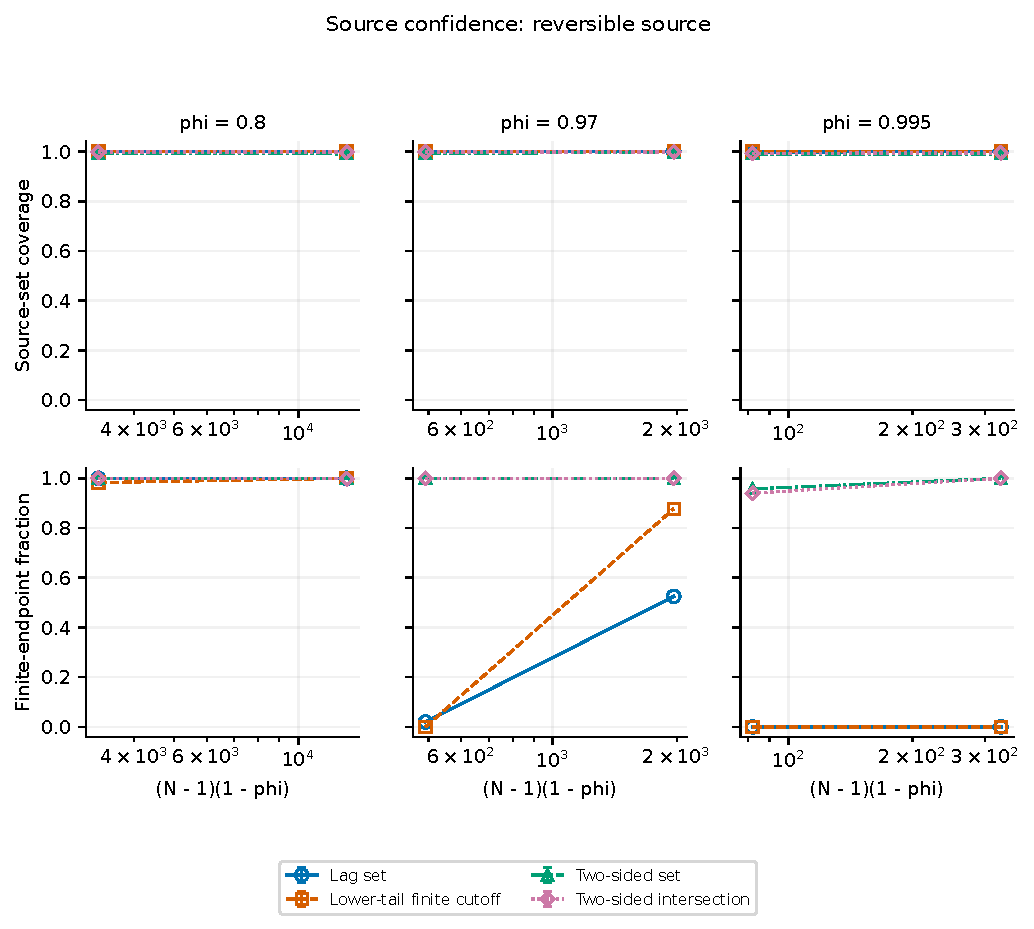
\includegraphics[width=7in]{figures/source_confidence_null.pdf}}
\caption{Coverage and finite endpoints differ across source constructions. Core null cells have 400 records, except $\phi=0.97,N=65537$, which has 1000. Coverage bars are pointwise 95\% binomial intervals. All fractions use the complete cell. The source confidence error is $0.005$, distinct from the display interval. Coincident curves have equal fractions; methods remain in the legend. Values are saved study results.}\label{fig:study16-source-null}
\end{figure}

\begin{figure}[p]
\centering
\makebox[\textwidth][c]{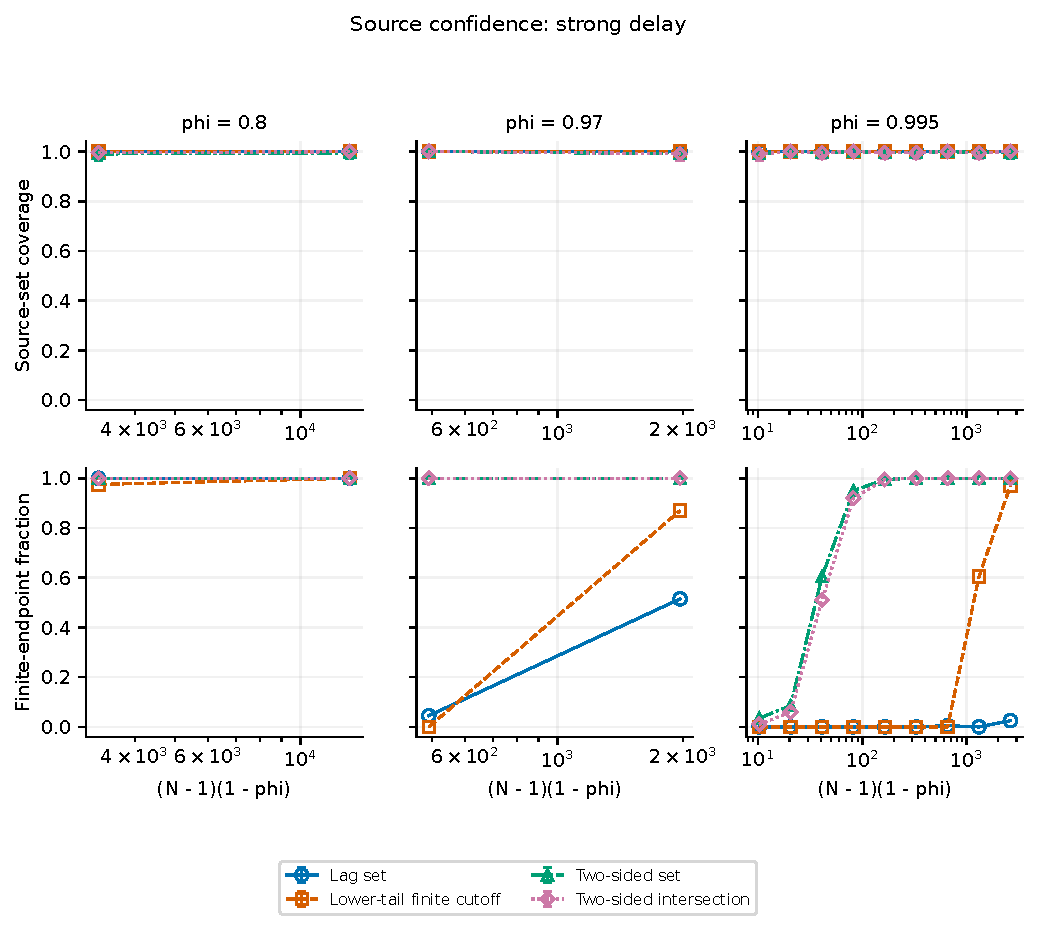
\includegraphics[width=7in]{figures/source_confidence_strong.pdf}}
\caption{Strong-delay records can have covered source sets without finite upper endpoints. Each condition has 200 records. The display includes the nine-length $\phi=0.995$ curve and both core lengths at other persistences. Coverage bars are pointwise 95\% binomial intervals; endpoint fractions use all records. Equal curves indicate equal fractions. The source-set error allowance is $0.005$. Values are saved study results.}\label{fig:study16-source-strong}
\end{figure}

\begin{figure}[p]
\centering
\makebox[\textwidth][c]{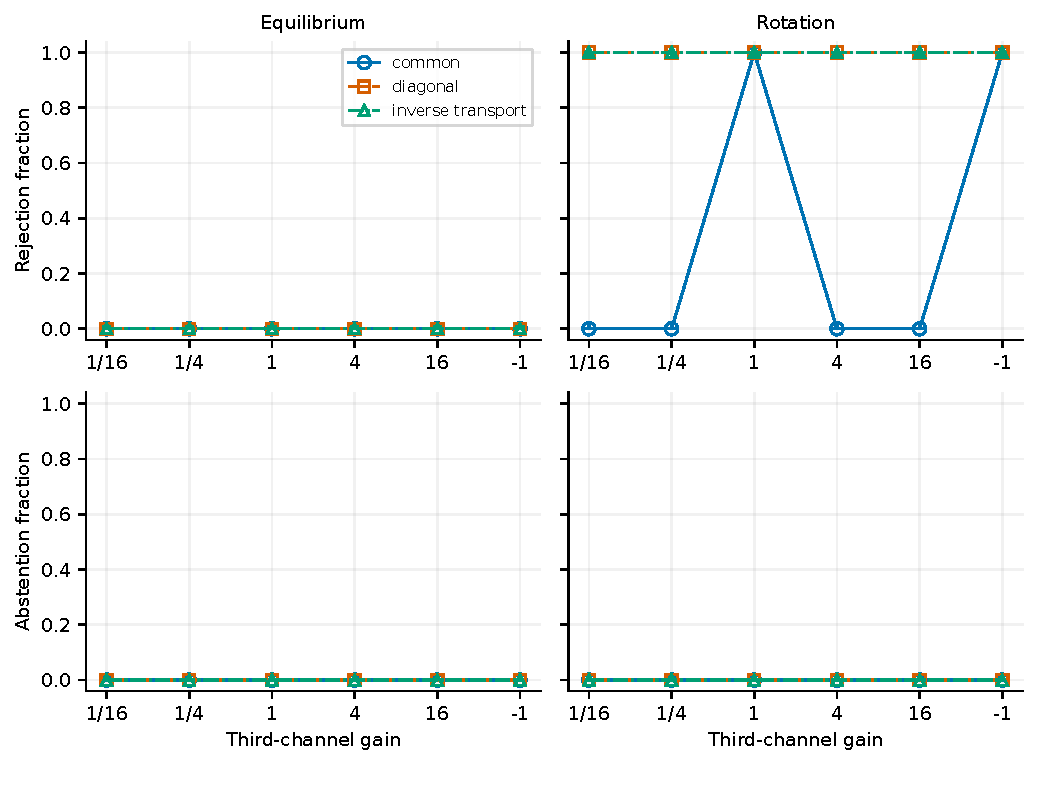
\includegraphics[width=7in]{figures/gain_controls.pdf}}
\caption{Diagonal bounds and inverse transport preserve all rotating-source rejections across six gains. The common scalar rule loses every rejection at four gains. Null and rotating cells have 400 and 200 records, respectively, with methods paired on each record. All abstention fractions and equilibrium rejection fractions are zero. These transformations change data and bounds together. Values are saved study results.}\label{fig:study16-gains}
\end{figure}

\begin{figure}[p]
\centering
\makebox[\textwidth][c]{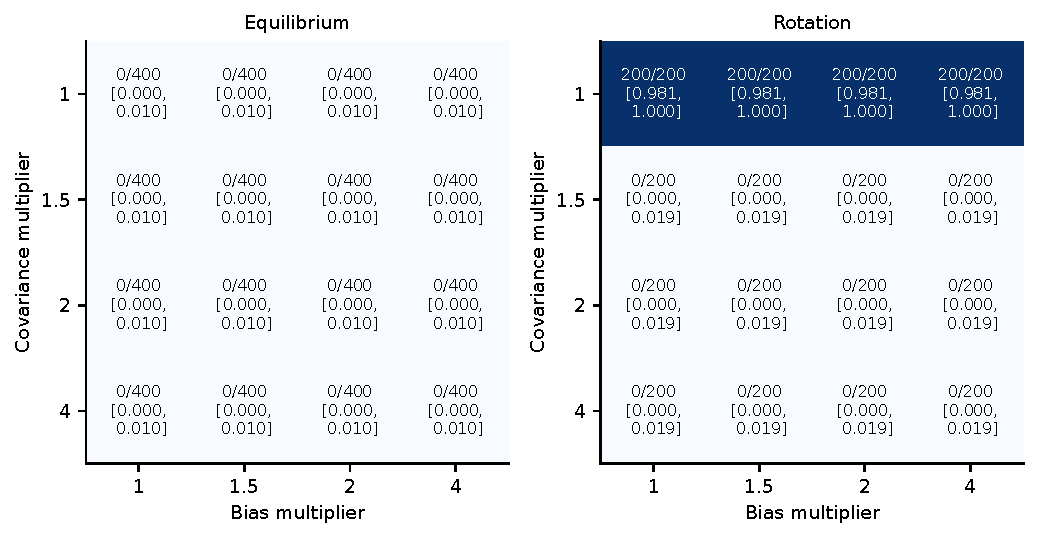
\includegraphics[width=7in]{figures/bound_inflation.pdf}}
\caption{Conservative covariance inflation removes rotating-source rejections within this grid. All 16 covariance/bias factor pairs are shown for both regimes, with 400 null or 200 rotating records. Entries give rejection counts and pointwise 95\% binomial intervals, rounded outward to $0.001$. No cell has an abstention. Equal counts across bias factors do not establish equal thresholds. Values are saved study results.}\label{fig:study16-inflation}
\end{figure}

\clearpage
\section{Source uncertainty and threshold diagnostics}\label{study16:diagnostics}
\subsection{Diagnostic question and definitions}\label{sec:src16:diagnostic-definitions}

A covered source hull enters the covariance envelope through its transformed span. A fixed bank adds a placement cost when none of its filters is close to the hull center in that transform. These costs determine the dependence bound used by the threshold, but an available threshold can still exceed the statistic. The diagnostics separate the remaining source uncertainty, the additional bank cost, and the final statistic-to-threshold comparison.

The hull-span ratio is $\Lambda(u)/\Lambda(\ell)$, with $\Lambda(x)=(1+x)/(1-x)$. It measures the source uncertainty that remains even if a common filter could be placed at the transformed hull center. The bank-placement factor divides the smallest source spectral-ratio bound in the fixed bank by this hull-span ratio. It measures the additional cost of the available filter positions. The final statistic-to-threshold ratio compares the selected absolute statistic with the upper threshold endpoint. The selected member has the largest saved statistic-minus-threshold margin among available members. A ratio above one supports rejection; a zero ratio is valid.

The diagnostics use all nine strong-delay lengths at persistence 0.995. Each condition has 200 independent records. The four source constructions are lag, lower-tail finite-cutoff, two-sided, and two-sided intersection. Each numerical summary uses only its saved finite values. Thus the records can differ between quantities and methods. Availability is part of the result, and every median must be read with its finite, missing, and full counts.

\paragraph{Display conventions.}
Figure~\ref{fig:src16:hull-bank-threshold} shows medians and ranges from the 25th to the 75th percentile in its upper panels. Its lower panels show the fraction of records with a finite saved value. Figure~\ref{fig:src16:threshold-components} shows finite-value medians and the same percentile ranges for the four threshold quantities. These ranges are descriptive summaries, not confidence intervals. A missing quantity has no plotted summary point and is not replaced by zero. A legend entry does not imply that a method has finite points at every length. The captions specify the axes, reference line, and method styles.

\subsection{Geometry and selected threshold quantities}\label{sec:src16:diagnostic-geometry}

The two-sided geometry summaries use 7 of 200 records at $N=2049$, 190 of 200 at $N=16385$, and all 200 at $N=524289$. The statistic-to-threshold ratio uses fewer records at the first two lengths. Table~\ref{tab:src16:geometry-examples} keeps each median beside its own counts. These different subsets show why finite geometry and an available threshold must be reported separately. The changing finite groups are not trajectories of the same records.

\begin{table}[!htbp]
\centering\small\setlength{\tabcolsep}{4pt}
\caption{Two-sided geometry and selected statistic-to-threshold medians at three strong-delay lengths and persistence 0.995. Each median uses only the finite values in its row. Finite, missing, and full record counts are adjacent. Geometry and threshold summaries can use different records.}\label{tab:src16:geometry-examples}
\begin{tabular}{@{}llrrrr@{}}
\toprule
$N$ & Quantity & Median & Finite & Missing & Full \\\midrule
2049 & Hull-span ratio & 67.2 & 7 & 193 & 200 \\
2049 & Bank-placement factor & 2.22 & 7 & 193 & 200 \\
2049 & Statistic-to-threshold ratio & 0.233 & 1 & 199 & 200 \\
\addlinespace
16385 & Hull-span ratio & 9.25 & 190 & 10 & 200 \\
16385 & Bank-placement factor & 1.96 & 190 & 10 & 200 \\
16385 & Statistic-to-threshold ratio & 1.95 & 182 & 18 & 200 \\
\addlinespace
524289 & Hull-span ratio & 7.45 & 200 & 0 & 200 \\
524289 & Bank-placement factor & 1.62 & 200 & 0 & 200 \\
524289 & Statistic-to-threshold ratio & 15.4 & 200 & 0 & 200 \\
\bottomrule\end{tabular}
\end{table}


The same summaries are much less available for lag and lower-tail inference. Both constructions have no finite plotted summaries at the first six lengths. At N=524289, the lag construction has only five finite values for each plotted quantity and 195 missing values. Its statistic-to-threshold median is 16.3. This median does not describe the other 195 records. The lower-tail construction has 194 finite geometry values and six missing values. Its hull-span median is 7.90e3. Its selected statistic-to-threshold median is 0.0929, based on 54 finite values and 146 missing values. These finite counts limit comparisons between the curves.

Among the finite selected two-sided members, the sampling-radius median decreases from 0.0378 to 0.000503 across these example lengths. The recorder-allowance median stays between 7.55e-7 and 7.60e-7. Table~\ref{tab:src16:threshold-examples} gives the intermediate values, phase allowances, and scale denominators with their counts. These summaries describe the saved selected members. They do not identify a cause for every decision.

\begingroup\small\setlength{\tabcolsep}{4pt}
\begin{longtable}{@{}llrrrr@{}}
\caption{Saved threshold quantities for the selected two-sided members at the same three strong-delay lengths and persistence 0.995. Allowances use saved upper endpoints. The scale denominator uses its saved lower endpoint. Each median uses only the finite values in its row.}\label{tab:src16:threshold-examples}\\
\toprule
$N$ & Quantity & Median & Finite & Missing & Full \\\midrule\endhead
2049 & Phase allowance & 2.92e-4 & 1 & 199 & 200 \\
2049 & Sampling radius & 0.0378 & 1 & 199 & 200 \\
2049 & Recorder allowance & 7.55e-7 & 1 & 199 & 200 \\
2049 & Scale denominator & 0.297 & 1 & 199 & 200 \\
\addlinespace
16385 & Phase allowance & 1.01e-4 & 182 & 18 & 200 \\
16385 & Sampling radius & 0.00452 & 182 & 18 & 200 \\
16385 & Recorder allowance & 7.59e-7 & 182 & 18 & 200 \\
16385 & Scale denominator & 0.757 & 182 & 18 & 200 \\
\addlinespace
524289 & Phase allowance & 7.59e-5 & 200 & 0 & 200 \\
524289 & Sampling radius & 0.000503 & 200 & 0 & 200 \\
524289 & Recorder allowance & 7.60e-7 & 200 & 0 & 200 \\
524289 & Scale denominator & 0.964 & 200 & 0 & 200 \\
\bottomrule\end{longtable}
\endgroup


\subsection{Weak-delay source confidence}\label{sec:src16:weak-confidence}

Figure ~\ref{fig:src16:source-confidence-weak} separates returned-set coverage from finite-endpoint availability. At persistence 0.995, lag and lower-tail sets cover the source value in 200/200 records at both fixed lengths. Neither has a finite endpoint in any record. The two-sided and intersection finite-endpoint counts are 185/200 and 180/200 at N=16385. Both are 200/200 at N=65537. At this longer length, their coverage counts are 198/200 and 199/200. The pointwise 95\% coverage intervals, rounded outward, are [0.964, 0.999] and [0.972, 1.000]. Thus full finite-endpoint availability does not mean observed coverage is 200/200.

At persistence 0.97 and $N=16385$, lag has 4/200 finite endpoints and lower-tail has 0/200. The two-sided and intersection constructions each have 200/200 finite endpoints. Their coverage counts are 199/200 for two-sided and 200/200 for intersection. At $N=65537$, the finite-endpoint counts are 107/200 for lag and 172/200 for lower-tail. Both two-sided constructions still have 200/200 finite endpoints. Coverage is 198/200 for two-sided and 199/200 for intersection.

At persistence 0.8, all constructions have coverage 200/200 at both lengths. All finite-endpoint counts are 200/200 except the lower-tail count of 199/200 at N=16385. The source-set error allowance is 0.005. It is distinct from the 95\% binomial display intervals. These empirical counts do not establish familywise coverage.

\subsection{First failed condition and available decisions}\label{sec:src16:first-failure}

The finite-value medians omit records where an earlier requirement prevented a saved value. The stacked bars in Figure~\ref{fig:src16:first-failure} restore those records to the comparison. A finite hull must still give a finite covariance bound and a positive scale denominator before the rule can compare its statistic with a threshold. The bars separate failures of these requirements from available nonrejections and rejections. The four panels compare lag, lower-tail finite-cutoff, two-sided, and two-sided intersection procedures across all nine strong-delay lengths at persistence 0.995. Every bar uses all 200 records in its condition.

Seven mutually exclusive categories cover the full sample: input or arithmetic failure, empty source set, a hull endpoint that reaches one, no finite covariance bound, no positive scale denominator, available nonrejection with insufficient margin, and rejection. For an unavailable decision, the category reports the first failed condition under the declared classification rule. It does not show that every other condition passed. Available nonrejection is distinct from abstention. Counts and full denominators remain in the complete tables. Category fractions are descriptive; the bars do not show confidence intervals. The caption specifies the visual styles.

Figure ~\ref{fig:src16:first-failure} retains all seven categories in all 36 method-condition groups. At N=2049, lag and lower-tail procedures both have 200 reported hull-endpoint first failures. The two-sided procedure has 193 such failures, six reported nonpositive scale-denominator first failures, and one available nonrejection. The intersection procedure has 198 hull-endpoint first failures, one nonpositive scale-denominator first failure, and one available nonrejection. None rejects in this condition.

At N=16385, the two-sided procedure has 153 rejections, 29 available nonrejections, and 18 abstentions. The abstentions comprise ten hull-endpoint first failures and eight nonpositive scale-denominator first failures. The intersection has 152 rejections, 22 available nonrejections, and 26 abstentions. Its abstentions comprise 16 hull-endpoint first failures and ten nonpositive scale-denominator first failures. Both procedures reject in all 200 records at each of the four longest lengths. At N=524289, lag has five rejections and 195 hull-endpoint first failures. Lower-tail has 54 available nonrejections and 146 abstentions. Those abstentions comprise six hull-endpoint first failures and 140 nonpositive scale-denominator first failures.

Input or arithmetic failure, empty source sets, and no finite covariance bound have zero reported first-failure counts in these 36 selected groups. The figure retains these categories. A reported nonpositive scale denominator does not establish saturation or a recording defect.

\subsection{Cycle radius terms}\label{sec:src16:cycle-terms}

The cycle threshold propagates complete edge radii through a product. Equal rejection counts under bias inflation therefore do not show that bias is absent or determine which term limits each record. The component summaries compare the terms entering those radii on the selected conditions, with all their finite-value counts retained.

The complete cycle-component CSV identified in Sec.~S11 retains the primary reversible and rotating conditions at N=131072. The file also retains both identity-detector conditions at N=2097152. It shows all three methods and all three edges. All 216 component-summary rows have finite values for the full condition sample. Their missing counts are zero. The full counts are 1000 for the primary reversible condition, 400 for the identity reversible condition, and 200 for each rotating condition.

Across all 36 selected cell-method-edge groups, the square-root sampling term has a larger median than each other non-total term. Table~\ref{tab:src16:cycle-examples} shows this comparison for the diagonal method and edge 1--2. It retains all six component medians in each of the four conditions, with each condition's counts.

\begingroup\small\setlength{\tabcolsep}{4pt}
\begin{longtable}{@{}llrrrr@{}}
\caption{Diagonal-method cycle-component medians for edge 1--2. Primary conditions use $N=131072$. Identity-detector conditions use $N=2097152$. Each median uses all records in its condition. The identity rotating medians round to the same displayed values as the identity reversible medians. Exact strings remain in the associated comma-separated-value (CSV) files.}\label{tab:src16:cycle-examples}\\
\toprule
Condition & Quantity & Median & Finite & Missing & Full \\\midrule\endhead
Primary reversible & Tail bias & 0.00115 & 1000 & 0 & 1000 \\
Primary reversible & Centering & 0.000973 & 1000 & 0 & 1000 \\
Primary reversible & Square-root sampling & 0.133 & 1000 & 0 & 1000 \\
Primary reversible & Linear sampling & 0.00251 & 1000 & 0 & 1000 \\
Primary reversible & Recording & 1.62e-5 & 1000 & 0 & 1000 \\
Primary reversible & Total & 0.138 & 1000 & 0 & 1000 \\
\addlinespace
Primary rotating & Tail bias & 0.00115 & 200 & 0 & 200 \\
Primary rotating & Centering & 0.000973 & 200 & 0 & 200 \\
Primary rotating & Square-root sampling & 0.133 & 200 & 0 & 200 \\
Primary rotating & Linear sampling & 0.00251 & 200 & 0 & 200 \\
Primary rotating & Recording & 1.61e-5 & 200 & 0 & 200 \\
Primary rotating & Total & 0.138 & 200 & 0 & 200 \\
\addlinespace
Identity reversible & Tail bias & 1.59e-5 & 400 & 0 & 400 \\
Identity reversible & Centering & 6.08e-5 & 400 & 0 & 400 \\
Identity reversible & Square-root sampling & 0.0333 & 400 & 0 & 400 \\
Identity reversible & Linear sampling & 0.000157 & 400 & 0 & 400 \\
Identity reversible & Recording & 1.62e-5 & 400 & 0 & 400 \\
Identity reversible & Total & 0.0336 & 400 & 0 & 400 \\
\addlinespace
Identity rotating & Tail bias & 1.59e-5 & 200 & 0 & 200 \\
Identity rotating & Centering & 6.08e-5 & 200 & 0 & 200 \\
Identity rotating & Square-root sampling & 0.0333 & 200 & 0 & 200 \\
Identity rotating & Linear sampling & 0.000157 & 200 & 0 & 200 \\
Identity rotating & Recording & 1.62e-5 & 200 & 0 & 200 \\
Identity rotating & Total & 0.0336 & 200 & 0 & 200 \\
\bottomrule\end{longtable}
\endgroup


The tail-bias medians remain positive even in the identity-detector conditions. The sampling-term comparison concerns descriptive medians. It does not establish a cause for each rejection or nonrejection. The component values were calculated from the declared formulas with Decimal50 arithmetic. They are not saved component enclosures. A median total need not equal the sum of component medians. These tables do not replace the separate cycle power result or turn its negative proof margins into a positive guarantee.

\begin{figure}[p]
\centering
\makebox[\textwidth][c]{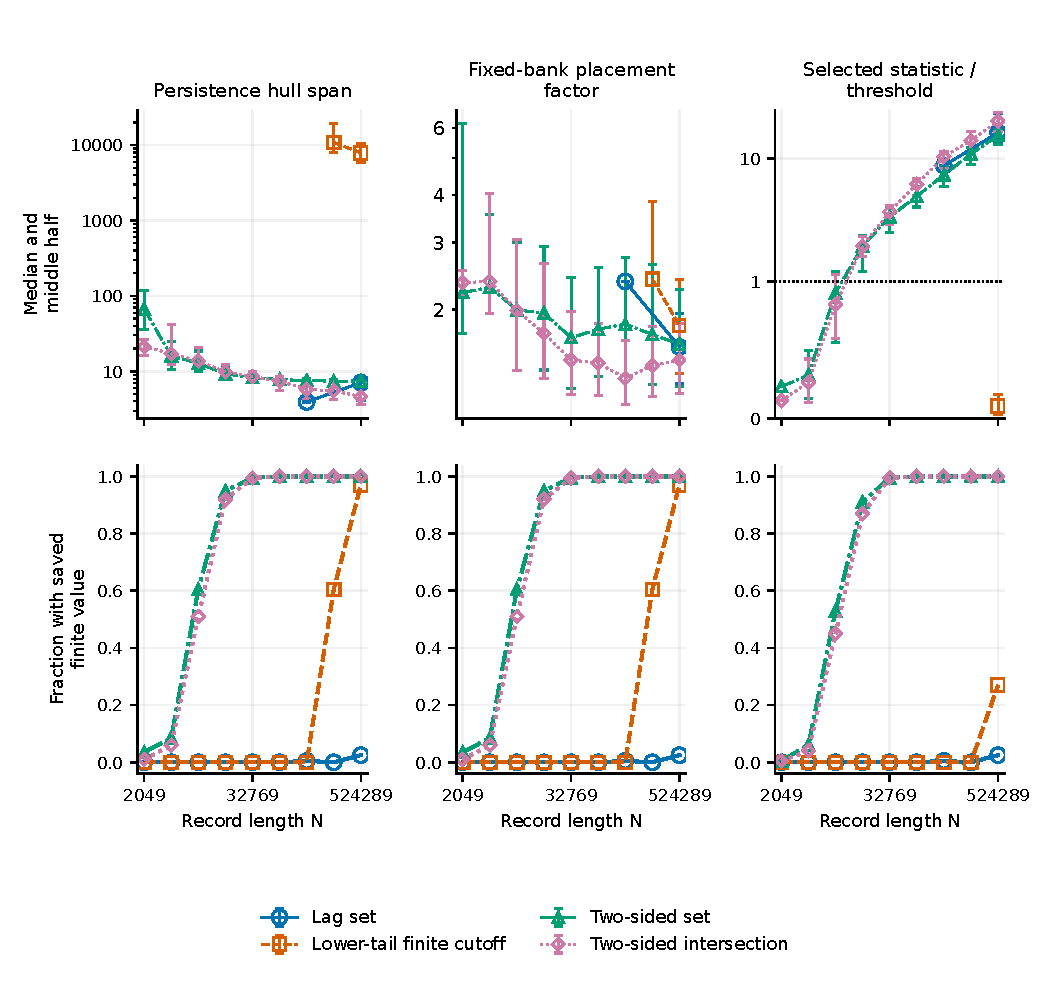
\includegraphics[width=7in]{figures/source_hull_bank_threshold.pdf}}
\caption{Finite source geometry and an available threshold occur on different record subsets. At $\phi=0.995$, each length has 200 records. Upper panels show finite-value medians and interquartile ranges; lower panels show finite-value fractions. The first two upper axes are logarithmic; the third is linear through one and logarithmic above it. Missing values are omitted, not zero. Section~\ref{sec:src16:diagnostic-definitions} defines the summaries.}\label{fig:src16:hull-bank-threshold}
\end{figure}

\begin{figure}[p]
\centering
\makebox[\textwidth][c]{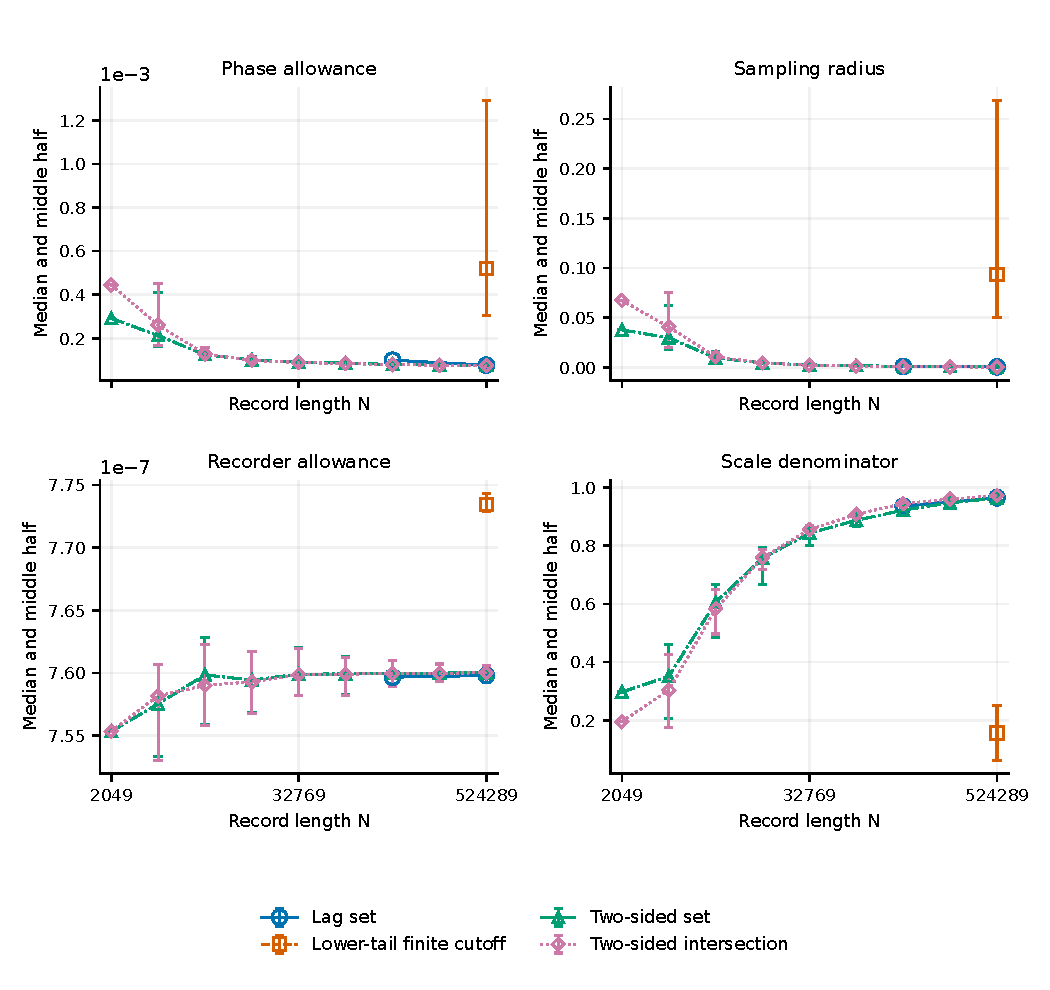
\includegraphics[width=6.8in]{figures/source_threshold_components.pdf}}
\caption{Median sampling allowances remain larger than median phase allowances in the selected two-sided members. At $\phi=0.995$, each length has 200 records. Curves give medians and interquartile ranges of saved finite values for the member with largest statistic-minus-threshold margin. Allowances use upper endpoints and denominators use lower endpoints. These ranges are descriptive, not confidence intervals. Missing values are omitted; a median total need not equal summed medians.}\label{fig:src16:threshold-components}
\end{figure}

\begin{figure}[p]
\centering
\makebox[\textwidth][c]{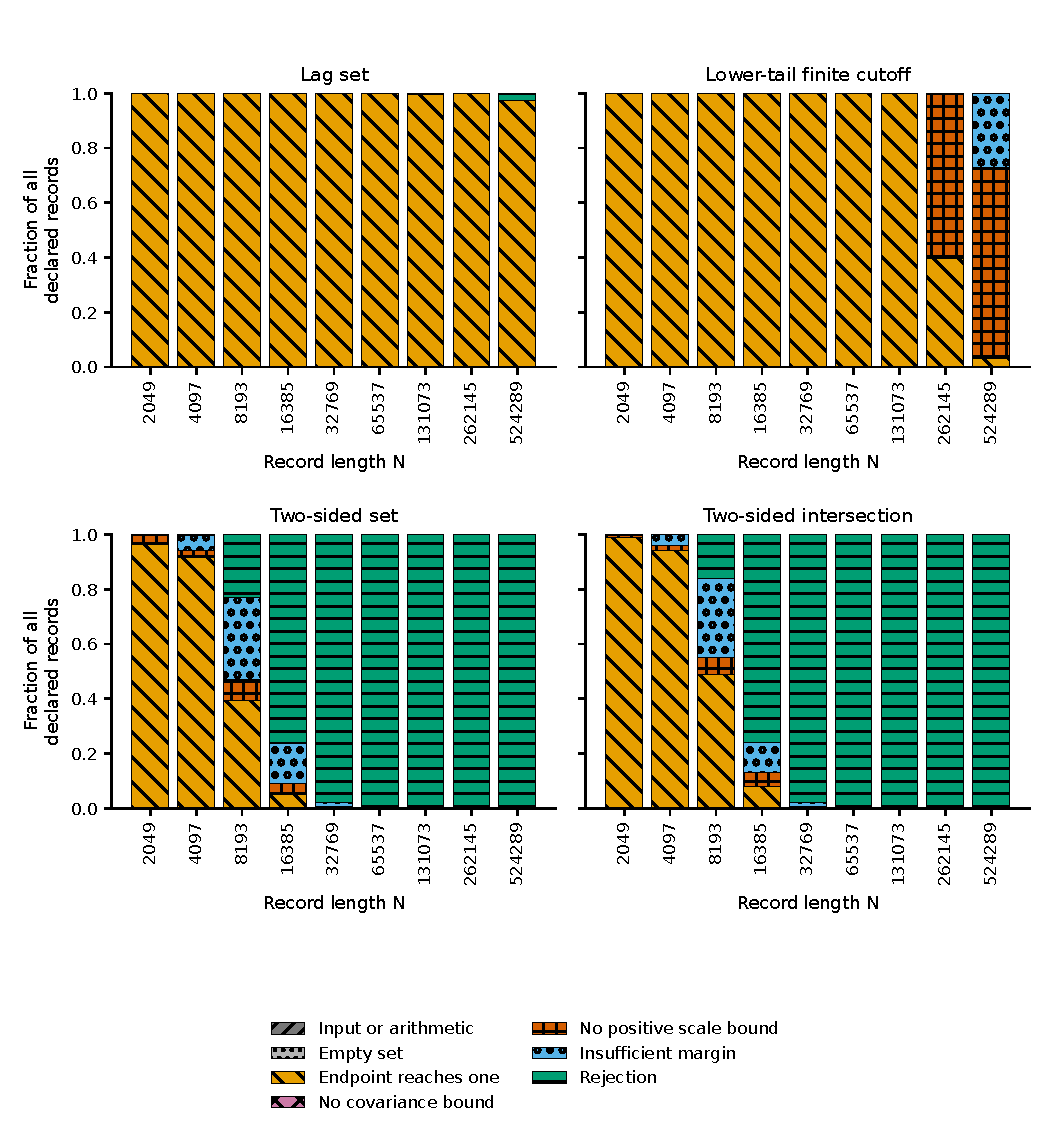
\includegraphics[width=7in]{figures/source_first_failure.pdf}}
\caption{The first failed condition separates unavailable tests from available nonrejections. Each bar uses all 200 records at one strong-delay length, with $\phi=0.995$. Seven mutually exclusive categories cover failures, nonrejections, and rejections, as defined in Sec.~\ref{sec:src16:first-failure}. A first failure does not imply that later requirements passed. Fractions are descriptive and carry no confidence intervals.}\label{fig:src16:first-failure}
\end{figure}

\begin{figure}[p]
\centering
\makebox[\textwidth][c]{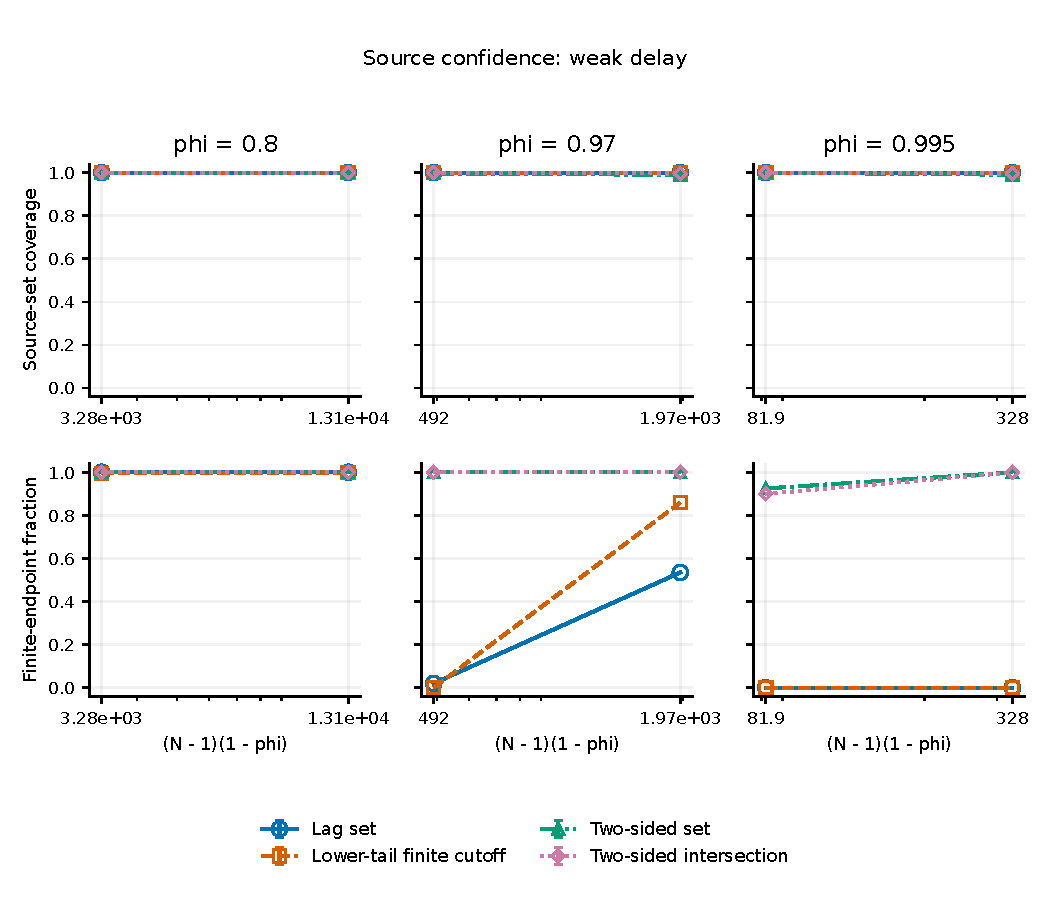
\includegraphics[width=7in]{figures/source_confidence_weak.pdf}}
\caption{Weak-delay source coverage and endpoint availability can differ sharply. Each cell has 200 records. Coverage bars are pointwise 95\% binomial intervals. Coverage and finite-endpoint fractions use the complete sample, while the confidence-set error allowance is $0.005$. At $\phi=0.995$, lag and lower-tail methods cover every source value but have no finite endpoint at either length. Coincident curves indicate equal fractions.}\label{fig:src16:source-confidence-weak}
\end{figure}

\clearpage
\section{Complete empirical tables and retained comparisons}\label{study16:tables}
The main comparisons are summarized in Secs.~S9--S10. The complete per-condition tables remain in the accompanying package under \texttt{results/current/tables/}. Table~\ref{tab:retained-csv} identifies the exact files. They retain full denominators, rejection/nonrejection/abstention counts, uncertainty intervals, and available-value counts. Paired differences use their separate companion files. No condition or adverse result is removed from those data.

\begin{table}[ht]\centering
\caption{Complete empirical tables in the reproducibility package. File names are relative to \texttt{results/current/tables/}.}\label{tab:retained-csv}
\begin{tabular}{p{.32\textwidth}p{.58\textwidth}}\toprule
Comparison & Files \\\midrule
Covariance and bias inflation & \texttt{inflation\_counts.csv}, \texttt{inflation\_pairs.csv}\\
Transported gains & \texttt{gain\_counts.csv}, \texttt{gain\_pairs.csv}\\
Numerical settings and recorders & \texttt{settings\_counts.csv}, \texttt{settings\_pairs.csv}\\
Assumption violations & \texttt{violations\_counts.csv}\\
Phase-boundary controls & \texttt{near\_boundary\_counts.csv}\\
All cycle-radius components & \texttt{cycle\_components.csv}\\\bottomrule
\end{tabular}
\end{table}

\subsection{Decision patterns retained by the complete tables}
The gain and inflation tables support different conclusions. Transporting a gain preserves the diagonal rule's mathematical decision, while assigning one common scalar ceiling to every channel can inflate the smaller-channel edges. All six diagonal gain variants retain $200/200$ rotating-source rejections; the common rule loses all rejections at four gains. Inflation of a valid bound remains conservative, but increasing its covariance factor from one to $1.5$ removes all rotating-source detections throughout the tested bias grid. Zero detections under an underestimated bound, by contrast, cannot validate that bound.

The settings table retains recorder failures alongside successful numerical refinements. At $\phi=0.97,N=65537$, all tested subdivision depths and arithmetic precisions give two-sided counts $0/1000/0$ under the null and $199/1/0$ under strong delay. Fractional eight-bit recording changes the strong-delay counts to $0/65/135$. Both finite-range recorders give $0/0/200$, because a valid perturbation certificate is unavailable. These triplets mean rejection/nonrejection/abstention and retain every record.

The assumption-violation table concerns procedures used outside their corresponding guarantees. Reference noise and Student-$t$ innovations produce no null rejections in these cells, but this observation does not extend Gaussian reference coverage. Correlated detector errors remove the source interpretation of the cycle. The phase-boundary table instead stays within a reversible-source model: calibrated and phase-adjusted procedures return $0/400/0$, while raw procedures return $400/0/0$ at each tested fraction of the phase tolerance. The raw procedures concern recorded asymmetry.

\subsection{Cycle component summaries}
The complete component table contains 216 rows with full finite-value counts and zero missing values in the selected conditions. The largest median non-total term in every cell-method-edge group is the square-root sampling term. Table~\ref{tab:src16:cycle-examples} retains representative diagonal-rule values in Sec.~S10.5. These are descriptive Decimal50 calculations from the formulas, not saved component enclosures. Their medians do not establish the cause of every decision, and a median total need not equal the sum of component medians.


\section{Earlier comparisons and the limits they identify}\label{study16:onesided}
Earlier comparisons support two requirements of the present tests: control the whole source-confidence set, and preserve separate channel scales in cycle bounds. They use different designs and must not be combined with the 69-condition study. Complete results, including unsuccessful cases, remain in the full local reproducibility package. The public release includes the comparison tables under \texttt{earlier\_studies/}. The Methods timing disclosure states which outcomes were available when later methods were developed.

\subsection{Finite source bounds can still prevent a decision}
An earlier six-member-bank comparison used a noiseless AR(1) reference at persistence $0.8$, $0.97$, or $0.995$. Each model cell had 32 records at nested lengths $16385$ and $65537$. A cumulative confidence method with only a lower-tail cutoff gave no rejections. It produced 274 finite upper endpoints but only 136 available tests across 576 outcomes. Its confidence hulls retained zero, leaving a large spectral range even after excluding persistence one. At $\phi=0.97,N=65537$, the median smallest bank source-ratio bound exceeded $4000$ in each regime. Thus a finite bound need not give a positive variance denominator or a useful threshold.

Intersecting confidence sets did not uniformly improve detection. In the strong-delay cell at $\phi=0.97,N=65537$, two records rejected only with the intersection and three only with lag confidence. The paired 95\% difference interval was $[-0.429,0.374]$. At $\phi=0.995$, all estimated methods abstained at both lengths, while the supplied-persistence control rejected every delayed alternative. All 18 population endpoint sufficient conditions failed. A separate comparison changed both the bank and calibration, so it could not isolate either change. All 144 sufficient power conditions were unavailable, and no record rejected only with estimated persistence. These results support controlling the full confidence hull without promising that an intersection always improves detection.

Complete outcomes and diagnostic quantities are in \texttt{earlier\_studies/source/analysis/}, including \texttt{method\_outcomes.csv}, \texttt{paired\_outcomes.csv}, and \texttt{member\_diagnostics.csv}. The earlier one-sided results are distinct from the later two-sided thresholds.

\subsection{Dependence and channel scale limit detection}
In a supplied-source comparison, all 30 reversible-source rate cells had zero rejections. At $\phi=0.5$ with identity responses, a supplied-marginal test rose from $2/400$ to $400/400$ detections between lengths 8192 and 32768; a floor-and-ceiling test detected none. At $\phi=0.9$, the supplied-marginal test detected no alternatives at the tested lengths. Filtering with the true persistence gave $400/400$ in every alternative cell. These differences concern the bounds supplied to that comparison.

An earlier cycle rule used one common radius for all channel pairs. Long rotating records with identity or unequal-delay detectors gave $64/64$ detections. Scaling only channel 3 to one quarter while retaining the common ceiling gave $0/32$; added noise gave $9/32$, and a response zero gave $0/32$. Short records gave no rejection. These results motivate separate channel bounds but do not evaluate the later common-family comparison. In a separate short-memory model, a certified population margin near $0.0332$ at length 131072 implied at least 80\% detection for the ideal mathematical rule. The other ten model-length conditions failed the sufficient inequality. This result did not establish completion of the bounded implementation. Model definitions and outcome tables are supplied under \texttt{earlier\_studies/mechanisms/study/}. Detailed per-record numerical files remain in the full local package.

\subsection{Planning bounds are conditional}
Earlier planning calculations checked sufficient inequalities without generating recordings. Of 360 white-marginal designs, joint phase-and-shape calibration with a Frobenius-only radius gave 208 sufficient cases. Including a trace bound gave 221, while 37 positive-gap cases still had no passing length. In 360 autoregressive cases, joint calibration gave 163 sufficient cases; 192 lacked a positive gap and five more lacked a passing length. The largest analytic length was $2147483648$; no such recording was generated. Complete designs and unsuccessful rows remain under \texttt{earlier\_studies/base/analysis/}. These calculations give neither physical recording durations nor performance guarantees for the present sharper tests.


\begingroup
\begin{thebibliography}{99}
\bibitem{taoequidistribution} \href{https://terrytao.wordpress.com/2010/03/28/254b-notes-1-equidistribution-of-polynomial-sequences-in-torii/}{Tao, T. 254B, Notes 1: Equidistribution of polynomial sequences in tori. 28 March 2010, Proposition 1 and Exercise 5.}
\bibitem{weyerfir} \href{https://doi.org/10.1109/CDC.2013.6761025}{Weyer, E., Cs\'aji, B. Cs. \& Campi, M. C. Guaranteed non-asymptotic confidence ellipsoids for FIR systems. In \emph{52nd IEEE Conference on Decision and Control}, 7162--7167 (2013).}
\bibitem{csajisps} \href{https://doi.org/10.1109/TSP.2014.2369000}{Cs\'aji, B. Cs., Campi, M. C. \& Weyer, E. Sign-Perturbed Sums: A new system identification approach for constructing exact non-asymptotic confidence regions in linear regression models. \emph{IEEE Trans. Signal Process.} \textbf{63}, 169--181 (2015).}
\bibitem{bomboisfrequency} \href{https://doi.org/10.1016/j.sysconle.2004.09.011}{Bombois, X., Anderson, B. D. O. \& Gevers, M. Quantification of frequency domain error bounds with guaranteed confidence level in prediction error identification. \emph{Systems \& Control Letters} \textbf{54}, 471--482 (2005).}
\bibitem{laurentmassart} \href{https://doi.org/10.1214/aos/1015957395}{Laurent, B. \& Massart, P. Adaptive estimation of a quadratic functional by model selection. \emph{Annals of Statistics} \textbf{28}, 1302--1338 (2000).}
\bibitem{kpss1992} \href{https://doi.org/10.1016/0304-4076(92)90104-Y}{Kwiatkowski, D., Phillips, P. C. B., Schmidt, P. \& Shin, Y. Testing the null hypothesis of stationarity against the alternative of a unit root: How sure are we that economic time series have a unit root? \emph{Journal of Econometrics} \textbf{54}, 159--178 (1992).}
\bibitem{imhof1961} \href{https://doi.org/10.1093/biomet/48.3-4.419}{J. P. Imhof, Computing the distribution of quadratic forms in normal variables, \emph{Biometrika} \textbf{48}, 419--426 (1961).}
\bibitem{davies1980} \href{https://doi.org/10.2307/2346911}{R. B. Davies, Algorithm AS 155: The distribution of a linear combination of chi-squared random variables, \emph{Applied Statistics} \textbf{29}, 323--333 (1980).}
\bibitem{dufourking1991} \href{https://doi.org/10.1016/0304-4076(91)90080-W}{Dufour, J.-M. \& King, M. L. Optimal invariant tests for the autocorrelation coefficient in linear regressions with stationary or nonstationary AR(1) errors. \emph{Journal of Econometrics} \textbf{47}, 115--143 (1991).}
\bibitem{elliott1996} \href{https://doi.org/10.2307/2171846}{G. Elliott, T. J. Rothenberg, and J. H. Stock, Efficient tests for an autoregressive unit root, \emph{Econometrica} \textbf{64}, 813--836 (1996).}
\bibitem{slepian1978} \href{https://doi.org/10.1002/j.1538-7305.1978.tb02104.x}{D. Slepian, Prolate spheroidal wave functions, Fourier analysis, and uncertainty. V. The discrete case, \emph{Bell System Technical Journal} \textbf{57}, 1371--1430 (1978).}
\bibitem{landauwidom1980} \href{https://doi.org/10.1016/0022-247X(80)90241-3}{H. J. Landau and H. Widom, Eigenvalue distribution of time and frequency limiting, \emph{Journal of Mathematical Analysis and Applications} \textbf{77}, 469--481 (1980).}
\bibitem{lecam1986} \href{https://doi.org/10.1007/978-1-4612-4946-7}{L. Le Cam, \emph{Asymptotic Methods in Statistical Decision Theory} (Springer, New York, 1986).}
\bibitem{seifert2012} \href{https://doi.org/10.1088/0034-4885/75/12/126001}{U. Seifert, Stochastic thermodynamics, fluctuation theorems and molecular machines, \emph{Reports on Progress in Physics} \textbf{75}, 126001 (2012).}
\bibitem{kunsch1989} \href{https://doi.org/10.1214/aos/1176347265}{H. R. K\"unsch, The jackknife and the bootstrap for general stationary observations, \emph{Annals of Statistics} \textbf{17}, 1217--1241 (1989).}
\bibitem{noltecoherency2004} \href{https://doi.org/10.1016/j.clinph.2004.04.029}{Nolte, G., Bai, O., Wheaton, L., Mari, Z., Vorbach, S. \& Hallett, M.
Identifying true brain interaction from EEG data using the imaginary part of coherency.
\emph{Clinical Neurophysiology} \textbf{115}, 2292--2307 (2004).}
\bibitem{clopper} \href{https://doi.org/10.1093/biomet/26.4.404}{Clopper, C. J. \& Pearson, E. S. The use of confidence or fiducial limits illustrated in the case of the binomial. \emph{Biometrika} \textbf{26}, 404--413 (1934).}
\bibitem{andrews1993} \href{https://doi.org/10.2307/2951781}{Andrews, D. W. K. Exactly Median-Unbiased Estimation of First Order Autoregressive/Unit Root Models. \emph{Econometrica} \textbf{61}, 139--165 (1993).}
\end{thebibliography}

\endgroup
\end{document}
